%============================================================================
% Project Report
% Design and Verification of a RISC-V Multiply-Accumulate (MAC) Unit
% for Digital Signal Processing
%
% Build:  pdflatex report.tex  (run twice for the table of contents)
%         or: latexmk -pdf report.tex
%============================================================================
\documentclass[11pt,a4paper]{report}

\usepackage[utf8]{inputenc}
\usepackage[T1]{fontenc}
\usepackage{lmodern}
\usepackage[margin=2.5cm]{geometry}
\usepackage{amsmath,amssymb}
\usepackage{graphicx}
\usepackage{booktabs}
\usepackage{array}
\usepackage{tabularx}
\usepackage{multirow}
\usepackage{float}
\usepackage{caption}
\usepackage{xcolor}
\usepackage{listings}
\usepackage{tikz}
\usetikzlibrary{arrows.meta,positioning,shapes.geometric,fit,calc}
\usepackage{pgfplots}
\pgfplotsset{compat=1.18}
\usepackage{pdflscape}
\usepackage{fancyhdr}
\usepackage{titlesec}
\usepackage[hidelinks]{hyperref}
\hypersetup{
  pdftitle={Design and Verification of a RISC-V Multiply-Accumulate (MAC) Unit for Digital Signal Processing},
  pdfauthor={Mohsin Mushtaq (2025MECECS001), Mubashir Karim Ganaie (2025MECECS005)},
  pdfsubject={Project report, Department of Electronics and Communications, NIT Srinagar},
  pdfkeywords={RISC-V, MAC, Booth multiplier, DSP, Verilog, Yosys, ECP5}
}

%---------------------------------------------------------------------------
% Style
%---------------------------------------------------------------------------
\definecolor{codebg}{RGB}{248,248,248}
\definecolor{kw}{RGB}{0,0,160}
\definecolor{cm}{RGB}{0,120,0}
\definecolor{accent}{RGB}{31,78,154}

\titleformat{\chapter}[hang]{\Huge\bfseries\color{accent}}{\thechapter}{0.6em}{}
\titlespacing*{\chapter}{0pt}{-20pt}{18pt}

\pagestyle{fancy}
\fancyhf{}
\fancyhead[L]{\small RISC-V MAC Unit for DSP}
\fancyhead[R]{\small\leftmark}
\fancyfoot[C]{\thepage}
\renewcommand{\headrulewidth}{0.4pt}

\lstdefinestyle{verilog}{
  language=Verilog,
  basicstyle=\ttfamily\scriptsize,
  keywordstyle=\color{kw}\bfseries,
  commentstyle=\color{cm},
  backgroundcolor=\color{codebg},
  frame=single, rulecolor=\color{gray!50},
  numbers=left, numberstyle=\tiny\color{gray}, numbersep=6pt,
  breaklines=true, columns=fullflexible, keepspaces=true,
  showstringspaces=false, tabsize=4,
  morekeywords={localparam,signed,generate,endgenerate,genvar,integer,time},
  literate={±}{{$\pm$}}1
}
\lstdefinestyle{log}{
  basicstyle=\ttfamily\tiny,
  backgroundcolor=\color{codebg},
  frame=single, rulecolor=\color{gray!50},
  breaklines=true, columns=fullflexible, keepspaces=true
}
\lstset{style=verilog}

\newcommand{\code}[1]{\texttt{#1}}
\renewcommand{\bibname}{References}

%===========================================================================
\begin{document}
%===========================================================================

%---------------------------------------------------------------------------
% Title page
%---------------------------------------------------------------------------
\begin{titlepage}
  \centering
  \vspace*{1.5cm}
  {\Large PROJECT REPORT\par}
  \vspace{1.2cm}
  {\color{accent}\rule{\linewidth}{1.2pt}\par}
  \vspace{0.4cm}
  {\huge\bfseries Design and Verification of a\\[4pt]
   RISC-V Multiply-Accumulate (MAC) Unit\\[4pt]
   for Digital Signal Processing\par}
  \vspace{0.4cm}
  {\color{accent}\rule{\linewidth}{1.2pt}\par}
  \vspace{1.5cm}
  {\large Hardware Description Language: Verilog (IEEE Std 1364-2005)\\
   Simulator: Icarus Verilog 12 \quad Waveforms: GTKWave\\
   Synthesis: Yosys 0.70 \quad Place \& route: nextpnr-ecp5\\
   Integrated in a 5-stage pipelined RV32IM processor\par}
  \vspace{2.2cm}
  {\large\textbf{Submitted by}\par}
  \vspace{6pt}
  {\large
   \begin{tabular}{@{}l@{\qquad}l@{}}
     Mohsin Mushtaq        & 2025MECECS001 \\
     Mubashir Karim Ganaie & 2025MECECS005 \\
   \end{tabular}\par}
  \vspace{1.2cm}
  {\large\textbf{Submitted to}\\[6pt]
   Dr.~Afshan Amin Khan\par}
  \vspace{1.6cm}
  {\large Department of Electronics and Communications\\[2pt]
   National Institute of Technology Srinagar\par}
  \vspace{0.8cm}
  {\normalsize Code: \url{https://github.com/mohsin2240/rv32-booth-mac}\par}
  \vfill
  {\large \today\par}
\end{titlepage}

%---------------------------------------------------------------------------
\begin{abstract}
\noindent
Multiply-accumulate (MAC) is the basic operation behind digital signal
processing (DSP) kernels such as FIR filters, dot products and matrix
multiplication. This project designs and verifies a MAC unit for RISC-V and
integrates it into a complete 5-stage pipelined RISC-V processor. The unit
implements eight R-type instructions in the RISC-V \code{custom-0} opcode
space. It provides a dedicated 64-bit accumulator with signed saturation and a
sticky overflow flag, together with unsigned modular accumulation, a Q15
fixed-point read-out matching the ARM CMSIS-DSP convention, a parameterised
radix-4 Modified Booth multiplier, and a two-stage pipeline that accepts one
instruction per cycle. Within the processor (IF/ID/EX/MEM/WB, RV32I plus RV32M
multiply, full forwarding and hazard detection), the unit's two stages coincide
with EX and MEM, so MAC instructions flow through the pipeline like ordinary
instructions.

At unit level, two self-checking testbenches with an independent reference
model perform 88{,}896 checks with zero errors; these include an exhaustive
8-bit multiplier test, analytical DSP benchmarks and a 3{,}000-instruction
random regression. At system level, real RISC-V programs produced by a
purpose-written assembler run on the processor, comprising an 18-part ISA and
hazard self-test and a 16-tap Q15 low-pass FIR filter over 128 samples. All
programs pass. The FIR output is bit-identical to the golden model and
attenuates the unwanted tone by 60.1\,dB. With the MAC instructions, the filter
runs 1.59$\times$ faster (looped) and 2.67$\times$ faster (unrolled) than the
same filter in plain RV32IM code, and pipeline diagrams reconstructed from the
simulation trace and VCD waveforms document the pipeline behaviour.

Finally, Yosys produces a latch-free MAC netlist of 9{,}532 gates and 179
flip-flops, which passes the full testbench at gate level. After
place-and-route with nextpnr on a Lattice ECP5 FPGA, the MAC unit runs at
56.4\,MHz (78.8\,MHz using hard DSP blocks), and the complete processor with
the MAC unit runs at 34.6\,MHz using 9\,\% of the device. RTL schematics,
floorplans, routing-density maps and critical-path analyses are included.
\end{abstract}

\tableofcontents
\listoffigures
\listoftables

%===========================================================================
\chapter{Introduction}
%===========================================================================

\section{Motivation}
Signal-processing algorithms spend most of their run time evaluating sums of
products. An $N$-tap finite impulse response (FIR) filter, for example,
computes
\begin{equation}
  y[n] = \sum_{k=0}^{N-1} h[k]\,x[n-k],
  \label{eq:fir}
\end{equation}
which needs $N$ multiplications and $N$ additions for every output sample.
Dedicated DSP processors therefore provide a single-cycle
\emph{multiply-accumulate} instruction $\mathrm{ACC} \leftarrow \mathrm{ACC} + a\cdot b$
together with a wide accumulator, so that long sums do not overflow.

RISC-V is an open, modular instruction-set architecture (ISA)~\cite{riscv}.
The base RV32I ISA and the standard \code{M} extension provide \code{mul},
\code{mulh} and \code{add}, but no fused multiply-accumulate and no 64-bit
accumulator. On RV32IM, accumulating one 32$\times$32-bit product into a
64-bit sum takes about six instructions. RISC-V explicitly reserves opcode
space for custom extensions~\cite{riscv}, and DSP-oriented RISC-V cores such
as PULP RI5CY / OpenHW CV32E40P use this approach to add MAC
instructions~\cite{gautschi,cv32e40p}.

\section{Objectives}
\begin{enumerate}
  \item Define a small, consistent RISC-V instruction-set extension for
        multiply-accumulate operations in the \code{custom-0} opcode space.
  \item Implement a synthesizable, pipelined MAC unit in Verilog with:
        a 64-bit accumulator, signed saturation, unsigned accumulation, and
        Q15 fixed-point support.
  \item Implement the multiplier using the radix-4 Modified Booth algorithm.
  \item Verify the design with self-checking testbenches, using directed,
        benchmark and constrained-random tests, and compare the results
        against an independent reference model and analytically known values.
  \item Document the results using terminal output, logs and simulation
        waveforms.
  \item Integrate the MAC unit into a 5-stage pipelined RISC-V processor and
        run real RISC-V DSP programs on it, measuring the speed-up over
        plain RV32IM code.
  \item Synthesise the MAC unit and the processor with Yosys, place and route
        them on an FPGA, and re-verify the synthesised netlist.
\end{enumerate}

\section{Report organisation}
The remainder of this report is organised as follows. Chapter~\ref{ch:theory}
presents the theory (MAC operations in DSP, RISC-V extensions, fixed-point
arithmetic, Booth multiplication and pipelining), and Chapter~\ref{ch:spec}
gives the instruction-set and interface specification. Chapter~\ref{ch:impl}
describes the MAC unit RTL implementation, while Chapter~\ref{ch:cpu} covers
its integration into the 5-stage RISC-V processor. Chapter~\ref{ch:verif} sets
out the verification methodology, Chapter~\ref{ch:results} reports the MAC unit
simulation results, and Chapter~\ref{ch:sysres} reports the processor-level
simulation results (pipeline diagrams, waveforms, DSP results and performance).
Chapter~\ref{ch:synth} presents the synthesis and FPGA implementation
(schematics, area, timing and floorplans), and Chapters~\ref{ch:disc}
and~\ref{ch:concl} give the discussion and conclusion. The appendices contain
the full source code, scripts, programs and logs.

%===========================================================================
\chapter{Background and Theory}\label{ch:theory}
%===========================================================================

\section{Multiply-accumulate in digital signal processing}
Table~\ref{tab:kernels} shows that common DSP kernels reduce to repeated MAC
operations. The MAC rate of a processor therefore largely sets its DSP
throughput, which is why DSP architectures are traditionally rated in
MAC operations per second.

\begin{table}[H]
  \centering
  \caption{Common DSP kernels expressed as multiply-accumulate operations.}
  \label{tab:kernels}
  \begin{tabular}{@{}lll@{}}
    \toprule
    Kernel & Expression & MACs per output \\
    \midrule
    FIR filter      & $y[n]=\sum_k h[k]x[n-k]$            & $N$ (taps) \\
    Dot product     & $s=\sum_i a_i b_i$                  & $N$ \\
    Correlation     & $r[l]=\sum_n x[n]\,y[n+l]$          & $N$ per lag \\
    Matrix multiply & $c_{ij}=\sum_k a_{ik}b_{kj}$        & $K$ \\
    Energy          & $E=\sum_n x[n]^2$                   & $N$ \\
    \bottomrule
  \end{tabular}
\end{table}

\section{The RISC-V ISA and custom extensions}
The RISC-V Unprivileged ISA~\cite{riscv} uses fixed 32-bit instructions with
a 7-bit major opcode in bits [6:0]. In the base opcode map, the major opcodes
\code{custom-0} (\code{0001011}) and \code{custom-1} (\code{0101011}) are
reserved for non-standard extensions and are guaranteed never to be used by
standard extensions. The R-type format, with fields \code{funct7}, \code{rs2},
\code{rs1}, \code{funct3}, \code{rd} and \code{opcode}, has two source
registers and one destination register, which suits binary arithmetic
operations. This project places all of its instructions in \code{custom-0}
and uses \code{funct3} to select the operation.

Related work: the PULP RI5CY core~\cite{gautschi} and its successor OpenHW
CV32E40P~\cite{cv32e40p} add Xpulp instructions such as \code{p.mac} and
\code{p.msu}, which accumulate into a general-purpose register. This design
instead uses a dedicated 64-bit accumulator, in the style of classic DSPs,
so that 32$\times$32-bit products can be accumulated at full precision.

\section{Fixed-point arithmetic and the Q15 format}
DSP code often uses fixed-point fractional formats instead of floating point.
In the Q15 format, a 16-bit two's-complement integer $X$ represents the real
value $X/2^{15}$, which lies in $[-1,\,1-2^{-15}]$. Multiplying two Q15
numbers gives a Q30 product:
\begin{equation}
  \frac{X_1}{2^{15}}\cdot\frac{X_2}{2^{15}} = \frac{X_1 X_2}{2^{30}}.
\end{equation}
To convert an accumulated Q30 sum back to Q15, shift it right arithmetically
by 15 bits and saturate it to the 16-bit range. This is exactly what the ARM
CMSIS-DSP library does in \code{arm\_fir\_q15}, using
\code{\_\_SSAT(acc >> 15, 16)} on a 64-bit accumulator~\cite{cmsis}. One
important corner case is $(-1.0)\times(-1.0)=+1.0$, which cannot be
represented in Q15 and must saturate to $32767/32768$.

\section{Accumulator width, guard bits and saturation}
A signed 32$\times$32-bit product needs at most 64 bits; its magnitude is at
most $2^{62}$, reached by $(-2^{31})^2$. Summing $N$ such products needs a
further $\lceil\log_2 N\rceil$ \emph{guard bits} to rule out overflow
completely. A 64-bit accumulator is enough for typical Q15 workloads (products
below $2^{30}$, leaving more than 30 guard bits), but it can overflow with
full-scale 32-bit operands. Two's-complement wrap-around would turn a small
overflow into a large error with the wrong sign, so DSP hardware uses
\emph{saturation arithmetic}: the result is clamped to the largest or smallest
representable value~\cite{lyons}.

Signed overflow of $S=A+P$, where $A$ and $P$ are 64-bit two's-complement
values, is detected by sign-extending both operands to 65 bits:
\begin{equation}
  S_{65} = \{A_{63},A\} + \{P_{63},P\},\qquad
  \mathit{ovf} = S_{65}[64] \oplus S_{65}[63],
\end{equation}
\begin{equation}
  \mathrm{sat}(S) =
  \begin{cases}
    \mathtt{0x7FFF\_FFFF\_FFFF\_FFFF} & \text{if } \mathit{ovf} \wedge S_{65}[64]=0,\\
    \mathtt{0x8000\_0000\_0000\_0000} & \text{if } \mathit{ovf} \wedge S_{65}[64]=1,\\
    S_{65}[63:0] & \text{otherwise.}
  \end{cases}
\end{equation}

\section{Radix-4 Modified Booth multiplication}
Booth's algorithm~\cite{booth} recodes the multiplier so that runs of ones need
fewer additions. MacSorley's radix-4 (``modified'') form~\cite{macsorley}
scans the multiplier $B$ in overlapping 3-bit groups
$\{b_{2i+1}, b_{2i}, b_{2i-1}\}$ with $b_{-1}=0$. Each group is recoded into a
digit $d_i\in\{-2,-1,0,+1,+2\}$:
\begin{equation}
  d_i = -2b_{2i+1} + b_{2i} + b_{2i-1},\qquad
  A\cdot B = \sum_{i=0}^{W/2-1} d_i\,A\,4^{i}.
\end{equation}
A $W$-bit multiplication therefore needs only $W/2$ partial products instead
of $W$, which halves the depth of the adder tree~\cite{parhami}. Each partial
product is $0$, $\pm A$ or $\pm 2A$, so it can be formed with a shift and
an optional negation. No real multiplication is required.

\begin{table}[H]
  \centering
  \caption{Radix-4 Booth recoding table.}
  \label{tab:booth}
  \begin{tabular}{@{}ccccc@{}}
    \toprule
    $b_{2i+1}$ & $b_{2i}$ & $b_{2i-1}$ & Digit $d_i$ & Partial product \\
    \midrule
    0&0&0& $\phantom{-}0$ & $0$ \\
    0&0&1& $+1$ & $+A$ \\
    0&1&0& $+1$ & $+A$ \\
    0&1&1& $+2$ & $+2A$ \\
    1&0&0& $-2$ & $-2A$ \\
    1&0&1& $-1$ & $-A$ \\
    1&1&0& $-1$ & $-A$ \\
    1&1&1& $\phantom{-}0$ & $0$ \\
    \bottomrule
  \end{tabular}
\end{table}

\paragraph{Worked example.}
Take $A=7$ and $B=-3$ with $W=6$, so $B=\mathtt{111101}_2$ and the extended
multiplier is $\mathtt{111101\,0}$. The groups, from LSB to MSB, are
$\mathtt{010}\rightarrow+1$, $\mathtt{110}\rightarrow-1$ and
$\mathtt{111}\rightarrow 0$. Hence
$A\cdot B = (+1)A\cdot 4^0 + (-1)A\cdot 4^1 + 0 = 7 - 28 = -21$, as expected.

\paragraph{Signed and unsigned operation on one multiplier.}
Booth recoding assumes two's-complement operands. For an \emph{unsigned}
32-bit multiplication, the operands are zero-extended to 34 bits, which makes
them non-negative signed numbers. For a signed multiplication they are
sign-extended. Using 34 bits instead of 33 also keeps $W$ even, as radix-4
recoding requires. The true product always fits in 64 bits, so the low 64
bits of the 68-bit result are exact in both cases.

\section{Pipelining}
Pipelining splits a datapath into stages separated by registers. This raises
the achievable clock frequency and lets a new operation start every cycle.
The MAC unit uses two stages: multiplication, then accumulation. Both the
accumulator read and write happen in the second stage, in program order, so
a dependent sequence such as \code{mac}, \code{mac}, \code{rdacc} needs no
forwarding paths and no pipeline stalls.

\paragraph{The 5-stage RISC pipeline.}
The classic RISC processor pipeline~\cite{patterson} has five stages:
instruction fetch (\emph{IF}), decode and register read (\emph{ID}), execute
or address computation (\emph{EX}), data memory access (\emph{MEM}) and
register write-back (\emph{WB}). Ideally, one instruction completes every cycle
(CPI\,=\,1), and three kinds of hazard can prevent this. Data hazards occur when
an instruction needs a result that has not been written back yet; they are
removed by \emph{forwarding} results from later pipeline registers, and only
when a value is produced too late, such as a load result at the end of MEM, is
a one-cycle \emph{stall} needed. Control hazards occur because the instructions
fetched after a taken branch are on the wrong path and must be \emph{flushed}.
Structural hazards occur when two instructions need the same resource in the
same cycle, and they are avoided by giving each stage its own resources.
Chapter~\ref{ch:cpu} applies these rules to a processor that contains the MAC
unit.

%===========================================================================
\chapter{Design Specification}\label{ch:spec}
%===========================================================================

\section{Instruction encoding}
All MAC instructions use the RISC-V R-type format with
\code{opcode = 0001011} (\code{custom-0}) and \code{funct7 = 0000000}
(Figure~\ref{fig:enc}).

\begin{figure}[H]
  \centering
  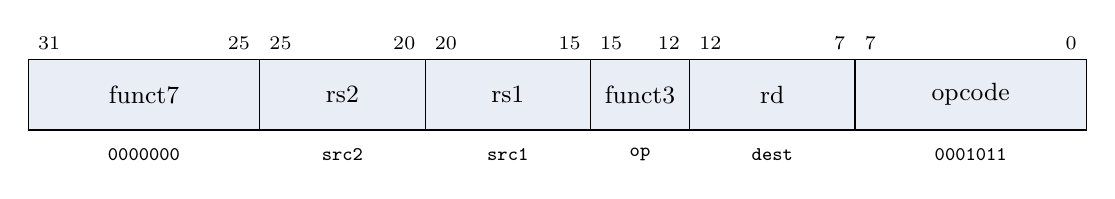
\begin{tikzpicture}[x=0.42cm,y=0.9cm,font=\small]
    \foreach \l/\r/\name/\val in {
        0/7/funct7/0000000, 7/12/rs2/src2, 12/17/rs1/src1,
        17/20/funct3/op, 20/25/rd/dest, 25/32/opcode/0001011} {
      \draw[fill=accent!10] (\l,0) rectangle (\r,1);
      \node at ({(\l+\r)/2},0.5) {\name};
      \node[font=\scriptsize\ttfamily] at ({(\l+\r)/2},-0.35) {\val};
    }
    \foreach \x/\b in {0/31,7/25,12/20,17/15,20/12,25/7} {
      \node[font=\scriptsize,anchor=south west] at (\x,1) {\b};
    }
    \foreach \x/\b in {7/25,12/20,17/15,20/12,25/7,32/0} {
      \node[font=\scriptsize,anchor=south east] at (\x,1) {\b};
    }
  \end{tikzpicture}
  \caption{R-type encoding of the MAC instructions (custom-0 major opcode).}
  \label{fig:enc}
\end{figure}

\section{Instruction set}
\begin{table}[H]
  \centering
  \caption{MAC unit instruction set. ACC is the 64-bit accumulator and OVF the sticky overflow flag.}
  \label{tab:isa}
  \small
  \begin{tabular}{@{}clll@{}}
    \toprule
    \code{funct3} & Assembly & Operation & Value written to \code{rd} \\
    \midrule
    000 & \code{mac rd,rs1,rs2}     & ACC $\leftarrow$ sat$_{64}$(ACC + rs1$\cdot$rs2), signed & ACC[31:0] \\
    001 & \code{msu rd,rs1,rs2}     & ACC $\leftarrow$ sat$_{64}$(ACC $-$ rs1$\cdot$rs2), signed & ACC[31:0] \\
    010 & \code{mul.acc rd,rs1,rs2} & ACC $\leftarrow$ rs1$\cdot$rs2; OVF $\leftarrow$ 0 & ACC[31:0] \\
    011 & \code{macu rd,rs1,rs2}    & ACC $\leftarrow$ ACC + rs1$\cdot$rs2, unsigned mod $2^{64}$ & ACC[31:0] \\
    100 & \code{rdacc.lo rd}        & read only & ACC[31:0] \\
    101 & \code{rdacc.hi rd}        & read only & ACC[63:32] \\
    110 & \code{rdacc.q15 rd}       & read only & sext(sat$_{16}$(ACC $\ggg$ 15)) \\
    111 & \code{clracc rd}          & ACC $\leftarrow$ 0; OVF $\leftarrow$ 0 & 0 \\
    \bottomrule
  \end{tabular}
\end{table}

\noindent Three additional rules complete the specification. As in all RISC-V
instructions, writes to \code{x0} are discarded (\code{rd\_we\_o = 0}), while
the accumulator is still updated. An instruction whose opcode is not
\code{custom-0}, or whose \code{funct7} is not zero, raises \code{illegal\_o}
and leaves the accumulator and flag unchanged; a core would turn this into an
illegal-instruction exception. Finally, OVF is set by any saturating
\code{mac}/\code{msu} and stays set until \code{clracc} or \code{mul.acc}, which
lets software check a whole dot product for overflow once, at the end.

\section{Module interface}
\begin{table}[H]
  \centering
  \caption{Port list of \code{mac\_unit}.}
  \label{tab:ports}
  \small
  \begin{tabularx}{\linewidth}{@{}llcX@{}}
    \toprule
    Port & Dir. & Width & Description \\
    \midrule
    \code{clk\_i}      & in  & 1  & Clock (rising-edge triggered) \\
    \code{rst\_ni}     & in  & 1  & Synchronous reset, active low \\
    \code{valid\_i}    & in  & 1  & An instruction and its operands are valid this cycle \\
    \code{instr\_i}    & in  & 32 & 32-bit RISC-V instruction word \\
    \code{rs1\_i}, \code{rs2\_i} & in & 32 & Operand values read from the register file \\
    \code{ready\_o}    & out & 1  & Always 1: the unit never stalls \\
    \code{valid\_o}    & out & 1  & Result valid (2 cycles after \code{valid\_i}) \\
    \code{rd\_addr\_o} & out & 5  & Destination register index \\
    \code{rd\_we\_o}   & out & 1  & Register-file write enable (0 for \code{x0} or illegal) \\
    \code{rd\_data\_o} & out & 32 & Value to write back \\
    \code{illegal\_o}  & out & 1  & Instruction is not a valid MAC instruction \\
    \code{ovf\_o}      & out & 1  & Sticky saturation flag \\
    \code{acc\_o}      & out & 64 & Current accumulator value (for debug and observability) \\
    \bottomrule
  \end{tabularx}
\end{table}

%===========================================================================
\chapter{Implementation}\label{ch:impl}
%===========================================================================

\section{Source files}
\begin{table}[H]
  \centering
  \caption{Project source files.}
  \label{tab:files}
  \small
  \begin{tabularx}{\linewidth}{@{}lX@{}}
    \toprule
    File & Contents \\
    \midrule
    \code{rtl/mac\_unit.v} & Main module: decoder, 2-stage pipeline, saturating accumulator, Q15 conversion \\
    \code{rtl/booth\_multiplier.v} & Parameterised radix-4 Booth multiplier (instantiated with $W=34$) \\
    \code{tb/tb\_mac\_unit.v} & Self-checking system testbench (reference model, scoreboard, 13 test groups) \\
    \code{tb/tb\_booth\_multiplier.v} & Multiplier unit testbench (exhaustive 8-bit, random 34-bit) \\
    \code{run\_sim.bat}, \code{run\_sim.sh} & Compile-and-run scripts for Icarus Verilog \\
    \code{synth/*.ys}, \code{run\_synth.sh} & Yosys synthesis scripts and the synthesis / P\&R / gate-level flow \\
    \code{synth/fmax\_wrapper.v} & Registered-I/O wrapper used only for timing analysis \\
    \code{rtl/rv32\_core.v}, \code{rtl/riscv\_soc.v} & 5-stage RV32IM processor with the integrated MAC unit, and its memories (Chapter~\ref{ch:cpu}) \\
    \code{tb/tb\_riscv\_soc.v} & System testbench that runs RISC-V programs on the processor \\
    \code{sw/*} & Assembler, build script, test and FIR programs, simulation runner \\
    \bottomrule
  \end{tabularx}
\end{table}

\section{Micro-architecture}
Figure~\ref{fig:arch} shows the datapath. Stage~1 decodes the instruction,
extends the operands and multiplies them. Stage~2 accumulates or reads out
the result and writes it back.

\begin{figure}[H]
  \centering
  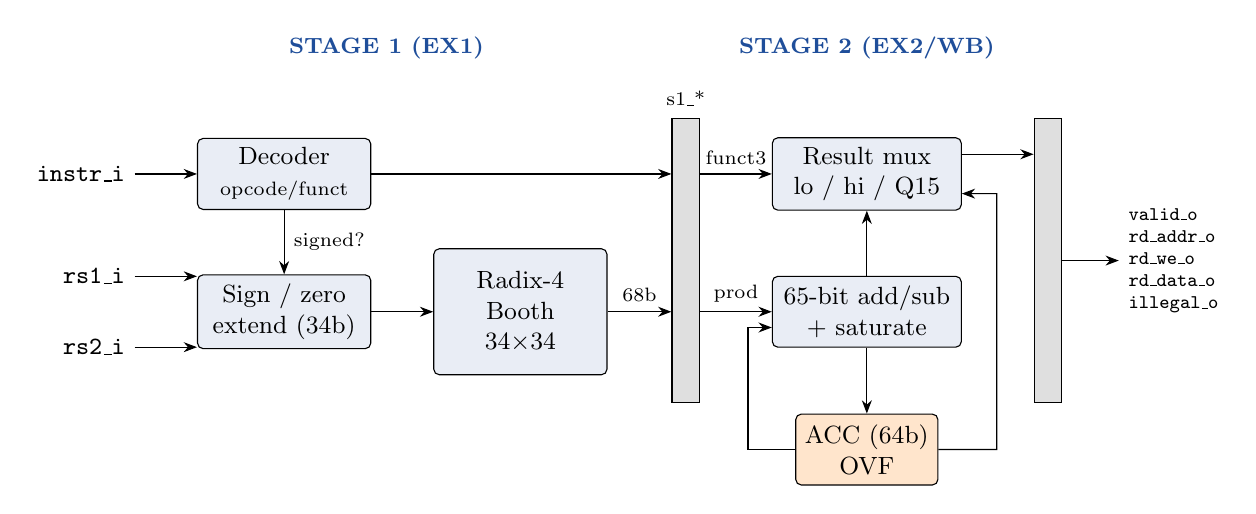
\begin{tikzpicture}[
      font=\small, >=Stealth,
      blk/.style={draw, fill=accent!10, rounded corners=2pt, minimum height=0.9cm, align=center},
      reg/.style={draw, fill=gray!25, minimum width=0.35cm, minimum height=3.6cm},
    ]
    % inputs
    \node[anchor=east] (in_i) at (0,2.2) {\code{instr\_i}};
    \node[anchor=east] (in_a) at (0,0.9) {\code{rs1\_i}};
    \node[anchor=east] (in_b) at (0,0.0) {\code{rs2\_i}};
    % stage 1
    \node[blk, minimum width=2.2cm] (dec) at (1.9,2.2) {Decoder\\\scriptsize opcode/funct};
    \node[blk, minimum width=2.2cm] (ext) at (1.9,0.45) {Sign / zero\\extend (34b)};
    \node[blk, minimum width=2.2cm, minimum height=1.6cm] (booth) at (4.9,0.45) {Radix-4\\Booth\\34$\times$34};
    % pipeline reg 1
    \node[reg] (r1) at (7.0,1.1) {};
    \node[font=\scriptsize, above=1pt of r1] {s1\_*};
    % stage 2
    \node[blk, minimum width=2.4cm] (add) at (9.3,0.45) {65-bit add/sub\\+ saturate};
    \node[blk, minimum width=2.4cm] (q15) at (9.3,2.2) {Result mux\\lo / hi / Q15};
    \node[blk, minimum width=1.4cm, fill=orange!20] (acc) at (9.3,-1.3) {ACC (64b)\\OVF};
    % pipeline reg 2
    \node[reg] (r2) at (11.6,1.1) {};
    % outputs
    \node[anchor=west, align=left, font=\scriptsize] (out) at (12.5,1.1)
       {\code{valid\_o}\\\code{rd\_addr\_o}\\\code{rd\_we\_o}\\\code{rd\_data\_o}\\\code{illegal\_o}};
    % wires
    \draw[->] (in_i) -- (dec);
    \draw[->] (in_a) -- (in_a -| ext.west);
    \draw[->] (in_b) -- (in_b -| ext.west);
    \draw[->] (dec.south) -- node[right,font=\scriptsize]{signed?} (ext.north);
    \draw[->] (ext) -- (booth);
    \draw[->] (booth) -- node[above,font=\scriptsize]{68b} (booth -| r1.west);
    \draw[->] (dec.east) -- (dec -| r1.west);
    \draw[->] (r1.east |- add) -- node[above,font=\scriptsize]{prod} (add);
    \draw[->] (r1.east |- q15) -- node[above,font=\scriptsize]{funct3} (q15);
    \draw[->] (add.south) -- (acc.north);
    % ACC read path into the result mux (enters lower half of its east side)
    \draw[->] (acc.east) -| (10.95,1.95) -- ($(q15.east)+(0,-0.25)$);
    % ACC feedback into the adder
    \draw[->] (acc.west) -- ++(-0.6,0) |- ($(add.west)+(0,-0.2)$);
    \draw[->] (add.north) -- (q15.south);
    % result to the write-back register (upper half of the east side)
    \draw[->] ($(q15.east)+(0,0.25)$) -- ($(r2.west |- q15.east)+(0,0.25)$);
    \draw[->] (r2.east) -- node[above,font=\scriptsize]{} (out.west);
    % stage labels
    \node[font=\bfseries\footnotesize, text=accent] at (3.2,3.8) {STAGE 1 (EX1)};
    \node[font=\bfseries\footnotesize, text=accent] at (9.3,3.8) {STAGE 2 (EX2/WB)};
  \end{tikzpicture}
  \caption{Two-stage MAC unit datapath. Grey bars are pipeline registers.}
  \label{fig:arch}
\end{figure}

\paragraph{Timing behaviour.}
The unit sustains a throughput of one instruction per clock cycle, since
\code{ready\_o} is tied to 1, and its latency is two cycles from
\code{valid\_i} to \code{valid\_o}. There are no hazards: every accumulator
access happens in stage~2 in program order, so the results of back-to-back
dependent instructions are always correct.

\section{Booth multiplier}
The multiplier is written as a behavioural but synthesizable loop that
explicitly forms each Booth partial product (Table~\ref{tab:booth}) and adds
it with weight $4^i$. A synthesis tool unrolls the loop into $W/2=17$
partial-product selectors and an adder tree.

\begin{lstlisting}[firstnumber=69, caption={Booth recoding loop in \code{booth\_multiplier.v}.}]
always @* begin
    acc = {2*W{1'b0}};
    for (i = 0; i < W/2; i = i + 1) begin
        grp = b_ext[2*i +: 3];
        case (grp)                                 // Booth recoding
            3'b000, 3'b111: pp = {2*W{1'b0}};     //  0
            3'b001, 3'b010: pp =  a_ext;          // +A
            3'b011:         pp =  a_ext <<< 1;    // +2A
            3'b100:         pp = -(a_ext <<< 1);  // -2A
            3'b101, 3'b110: pp = -a_ext;          // -A
            default:        pp = {2*W{1'b0}};
        endcase
        acc = acc + (pp <<< (2*i));               // weight 4^i
    end
    p_o = acc;
end
\end{lstlisting}

\section{Stage 1: decode and multiply}
The decoder pulls the opcode, \code{funct3}, \code{funct7} and \code{rd} out of
the instruction word. The flag \code{is\_mac\_instr} is true only when the
opcode is \code{custom-0} and \code{funct7} is zero. For \code{macu} the
operands are zero-extended; for every other operation they are sign-extended.
At the end of the stage, the low 64 bits of the product, \code{funct3},
\code{rd}, the valid bit and the illegal flag are registered.

\begin{lstlisting}[caption={Operand extension and multiplier instantiation.}]
wire is_unsigned = (funct3 == F3_MACU);
wire [33:0] op_a = is_unsigned ? {2'b00, rs1_i} : {{2{rs1_i[31]}}, rs1_i};
wire [33:0] op_b = is_unsigned ? {2'b00, rs2_i} : {{2{rs2_i[31]}}, rs2_i};

booth_multiplier #(.W(34)) u_booth (.a_i(op_a), .b_i(op_b), .p_o(prod_full));
\end{lstlisting}

\section{Stage 2: accumulate, saturate and read out}
Stage~2 implements the overflow detection and saturation from
Section~2.4, using 65-bit sign-extended addition and subtraction.

\begin{lstlisting}[caption={Saturating accumulation and Q15 conversion.}]
wire signed [64:0] sum_add  = acc_ext + prod_ext;
wire signed [64:0] sum_sub  = acc_ext - prod_ext;
wire ovf_add = sum_add[64] ^ sum_add[63];
wire ovf_sub = sum_sub[64] ^ sum_sub[63];
wire [63:0] sat_add = ovf_add ? (sum_add[64] ? ACC_MIN : ACC_MAX) : sum_add[63:0];
wire [63:0] sat_sub = ovf_sub ? (sum_sub[64] ? ACC_MIN : ACC_MAX) : sum_sub[63:0];

// Q30 -> Q15 (CMSIS-DSP convention: __SSAT(acc >> 15, 16))
wire signed [63:0] acc_shr15 = acc_q >>> 15;
wire [15:0] q15_val = (acc_shr15 >  64'sd32767) ? 16'h7FFF :
                      (acc_shr15 < -64'sd32768) ? 16'h8000 : acc_shr15[15:0];
\end{lstlisting}

A combinational \code{case} statement on \code{funct3} chooses the next
accumulator value, the next OVF value and the result. On the clock edge these
are registered together with \code{valid\_o}, \code{rd\_addr\_o},
\code{rd\_we\_o = valid \& \textasciitilde illegal \& (rd != 0)} and
\code{illegal\_o}. The complete code is listed in Appendix~\ref{app:src}.

\section{Coding guidelines followed}
The RTL uses only synthesizable Verilog-2005 constructs, with no delays, no
initial blocks and no vendor primitives. Sequential logic uses non-blocking
assignments, whereas combinational logic uses \code{always @*} with default
assignments, so that no latches are inferred. Reset is synchronous and active
low, and all encodings are named \code{localparam} constants. Every file starts
with a header describing its purpose, ports and parameters, and the code is
commented inline. Compiling with \code{iverilog -Wall} produces no warnings.

%===========================================================================
\chapter{RISC-V Pipelined Processor Integration}\label{ch:cpu}
%===========================================================================

A MAC unit is only useful inside a processor that fetches, decodes and
issues its instructions. To show this, the MAC unit was built into a complete
\textbf{5-stage pipelined RISC-V processor} (\code{rtl/rv32\_core.v}, 638
lines) that implements RV32I, the multiply subset of RV32M, and the eight MAC
instructions of Chapter~\ref{ch:spec}. The processor runs real RISC-V machine
code produced by a purpose-written assembler. Its results are checked
bit-exactly in simulation (Chapter~\ref{ch:sysres}) and it was synthesised and
placed-and-routed on an FPGA (Chapter~\ref{ch:synth}).

\section{Pipeline organisation}
Figure~\ref{fig:cpu} shows the datapath. It is the classic five-stage RISC
pipeline (IF, ID, EX, MEM, WB) described by Patterson and
Hennessy~\cite{patterson}, extended with the MAC unit.

\begin{figure}[H]
  \centering
  \resizebox{\linewidth}{!}{% ===========================================================================
% fig_pipeline.tex - 5-stage RV32IM pipeline with the integrated MAC unit
% (included from report.tex)
% ===========================================================================
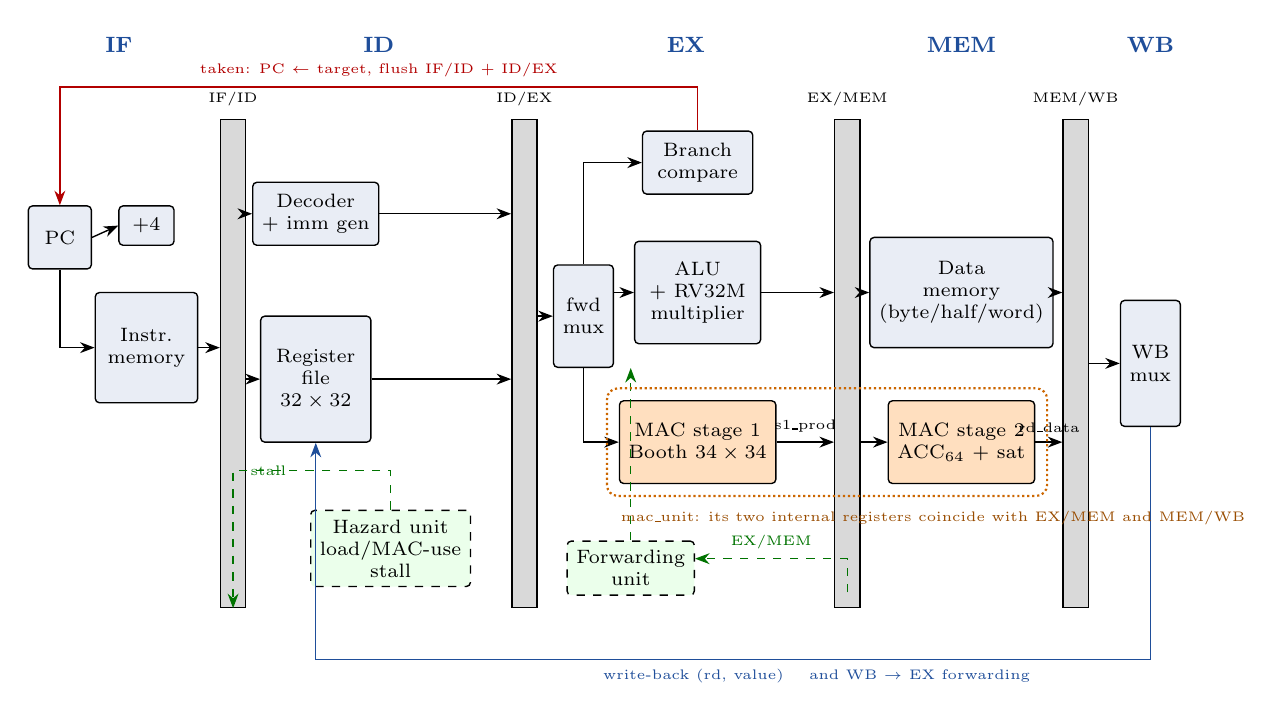
\begin{tikzpicture}[
    font=\scriptsize, >=Stealth, line width=0.5pt,
    blk/.style={draw, rounded corners=1.5pt, fill=accent!10, align=center, minimum height=0.8cm},
    mac/.style={draw, rounded corners=1.5pt, fill=orange!25, align=center},
    preg/.style={draw, fill=gray!30, minimum width=0.32cm, minimum height=6.2cm},
    unit/.style={draw, dashed, rounded corners=1.5pt, fill=green!8, align=center},
    lab/.style={font=\bfseries\footnotesize, text=accent},
  ]
  % ---------------- pipeline registers ----------------
  \node[preg] (r1) at (2.55,0) {};
  \node[preg] (r2) at (6.25,0) {};
  \node[preg] (r3) at (10.35,0) {};
  \node[preg] (r4) at (13.25,0) {};
  \node[font=\tiny, above=1pt of r1] {IF/ID};
  \node[font=\tiny, above=1pt of r2] {ID/EX};
  \node[font=\tiny, above=1pt of r3] {EX/MEM};
  \node[font=\tiny, above=1pt of r4] {MEM/WB};

  % ---------------- stage labels ----------------
  \node[lab] at (1.1,4.05)  {IF};
  \node[lab] at (4.4,4.05)  {ID};
  \node[lab] at (8.3,4.05)  {EX};
  \node[lab] at (11.8,4.05) {MEM};
  \node[lab] at (14.2,4.05) {WB};

  % ---------------- IF ----------------
  \node[blk, minimum width=0.8cm] (pc) at (0.35,1.6) {PC};
  \node[blk, minimum width=1.3cm, minimum height=1.4cm] (imem) at (1.45,0.2) {Instr.\\memory};
  \node[blk, minimum width=0.7cm, minimum height=0.5cm] (add4) at (1.45,1.75) {+4};
  \draw[->] (pc.south) |- (imem.west);
  \draw[->] (pc.east) -- (add4.west);
  \draw[->] (imem.east) -- (imem.east -| r1.west);

  % ---------------- ID ----------------
  \node[blk, minimum width=1.4cm] (dec) at (3.6,1.9) {Decoder\\+ imm gen};
  \node[blk, minimum width=1.4cm, minimum height=1.6cm] (rf) at (3.6,-0.2) {Register\\file\\$32\times32$};
  \node[unit, minimum width=1.5cm] (haz) at (4.55,-2.35) {Hazard unit\\load/MAC-use\\stall};
  \draw[->] (r1.east |- dec.west) -- (dec.west);
  \draw[->] (r1.east |- rf.west) -- (rf.west);
  \draw[->] (dec.east) -- (dec.east -| r2.west);
  \draw[->] (rf.east) -- (rf.east -| r2.west);

  % ---------------- EX ----------------
  \node[blk, minimum width=0.55cm, minimum height=1.3cm] (fmux) at (7.0,0.6) {fwd\\mux};
  \node[blk, minimum width=1.6cm, minimum height=1.3cm] (alu) at (8.45,0.9) {ALU\\+ RV32M\\multiplier};
  \node[blk, minimum width=1.4cm] (br) at (8.45,2.55) {Branch\\compare};
  \node[mac, minimum width=1.6cm, minimum height=1.05cm] (mac1) at (8.45,-1.0) {MAC stage 1\\Booth $34\times34$};
  \node[unit, minimum width=1.5cm] (fwd) at (7.6,-2.6) {Forwarding\\unit};
  \draw[->] (r2.east |- fmux.west) -- (fmux.west);
  \draw[->] (fmux.east |- alu.west) -- (alu.west);
  \draw[->] (fmux.north) |- (br.west);
  \draw[->] (fmux.south) |- (mac1.west);
  \draw[->] (alu.east) -- (alu.east -| r3.west);
  \draw[->] (mac1.east) -- node[above, font=\tiny]{s1\_prod} (mac1.east -| r3.west);
  \draw[->, red!70!black] (br.north) -- ++(0,0.55) -| node[pos=0.25, above, font=\tiny]{taken: PC $\leftarrow$ target, flush IF/ID + ID/EX} (pc.north);

  % ---------------- MEM ----------------
  \node[blk, minimum width=1.5cm, minimum height=1.4cm] (dmem) at (11.8,0.9) {Data\\memory\\(byte/half/word)};
  \node[mac, minimum width=1.5cm, minimum height=1.05cm] (mac2) at (11.8,-1.0) {MAC stage 2\\ACC$_{64}$ + sat};
  \draw[->] (r3.east |- dmem.west) -- (dmem.west);
  \draw[->] (r3.east |- mac2.west) -- (mac2.west);
  \draw[->] (dmem.east) -- (dmem.east -| r4.west);
  \draw[->] (mac2.east) -- node[above, font=\tiny]{rd\_data} (mac2.east -| r4.west);

  % ---------------- WB ----------------
  \node[blk, minimum width=0.6cm, minimum height=1.6cm] (wbmux) at (14.2,0.0) {WB\\mux};
  \draw[->] (r4.east |- wbmux.west) -- (wbmux.west);
  % write-back to register file
  \draw[->, accent] (wbmux.south) -- ++(0,-2.95) -| node[pos=0.2, below, font=\tiny]{write-back (rd, value) \quad and WB $\rightarrow$ EX forwarding} (rf.south);

  % forwarding paths (dashed)
  \draw[->, dashed, green!45!black] (r3.south) ++(0,0.2) |- ($(fwd.east)+(0,0.12)$) node[pos=0.75, above, font=\tiny]{EX/MEM};
  \draw[->, dashed, green!45!black] (fwd.north) -- (fwd.north |- fmux.south);
  \draw[->, dashed, green!45!black] (haz.north) -- ++(0,0.5) -| node[pos=0.3, left, font=\tiny]{stall} (r1.south);

  % MAC span box
  \draw[orange!80!black, rounded corners, densely dotted, line width=0.8pt]
      ($(mac1.south west)+(-0.15,-0.15)$) rectangle ($(mac2.north east)+(0.15,0.15)$);
  \node[font=\tiny, text=orange!60!black, anchor=north west] at ($(mac1.south west)+(-0.1,-0.22)$)
      {mac\_unit: its two internal registers coincide with EX/MEM and MEM/WB};
\end{tikzpicture}
}
  \caption{5-stage RV32IM pipeline with the integrated MAC unit. Grey bars are
    pipeline registers; dashed green blocks are the hazard and forwarding
    units; the MAC unit (orange) spans EX and MEM.}
  \label{fig:cpu}
\end{figure}

\begin{table}[H]
  \centering
  \caption{Work done in each pipeline stage.}
  \label{tab:stages}
  \small
  \begin{tabularx}{\linewidth}{@{}lXX@{}}
    \toprule
    Stage & Ordinary instructions & MAC instructions \\
    \midrule
    IF  & PC register addresses the instruction memory; next PC = PC+4 or branch target & same \\
    ID  & decode, immediate generation, register-file read (with write-first bypass), hazard check & same; only \code{mac/msu/mul.acc/macu} read \code{rs1}/\code{rs2} \\
    EX  & forwarding muxes, ALU, RV32M multiplier, branch/jump resolution & forwarded operands enter \textbf{MAC stage 1}: decode + Booth multiply \\
    MEM & load/store access with byte/half/word alignment & \textbf{MAC stage 2}: accumulate, saturate, read-out \\
    WB  & write ALU result or load data to \code{rd} & write the MAC result to \code{rd} \\
    \bottomrule
  \end{tabularx}
\end{table}

\paragraph{Why the MAC unit fits without stalls.}
The MAC unit has two internal pipeline registers (Chapter~\ref{ch:impl}). In
the processor they line up exactly with the EX/MEM and MEM/WB registers: a MAC
instruction is in MAC stage~1 while it is in EX, in MAC stage~2 while it is in
MEM, and its \code{rd\_data\_o} is valid when it reaches WB. The MAC unit
never stalls, and the core never stalls EX, MEM or WB, so the two pipelines
always move together. The testbench checks this alignment on every MAC
write-back.

\section{Hazard handling}
\paragraph{Data hazards: forwarding.}
An instruction in EX can read a value that has been computed but not yet
written to the register file. The forwarding unit selects each EX operand
from three sources, in priority order:
\begin{equation}
  \text{op}_A =
  \begin{cases}
    \text{EX/MEM.result} & \text{if EX/MEM writes } rd = rs_1 \ne 0 \text{ and is not a load or MAC},\\
    \text{WB value}      & \text{else if MEM/WB writes } rd = rs_1 \ne 0,\\
    \text{ID/EX.rs1\_val} & \text{otherwise,}
  \end{cases}
\end{equation}
and the same for $\text{op}_B$. The register file is also bypassed in ID, so
an instruction three positions behind a writer always reads the new value.

\paragraph{Load-use and MAC-use stalls.}
A load result is ready only at the end of MEM, and so is a MAC result, because
it leaves MAC stage~2 at the MEM/WB boundary. An instruction that uses such a
result immediately afterwards must therefore wait one cycle. The hazard unit
detects
\begin{equation}
\begin{split}
  \text{stall} = {} & \text{IF/ID.valid} \wedge \text{ID/EX.valid} \wedge
                      (\text{ID/EX.load} \vee \text{ID/EX.mac}) \\
                    & \wedge \big(rd_{EX}=rs_{1,ID} \vee rd_{EX}=rs_{2,ID}\big) \wedge rd_{EX}\ne 0,
\end{split}
\end{equation}
freezes PC and IF/ID, and inserts a bubble into ID/EX. One cycle later, the
value is forwarded from WB. Section~\ref{sec:pipeviz} shows this happening in
the simulation.

\paragraph{Control hazards.}
Branches and jumps are resolved in EX. A taken branch loads the target into
the PC and turns the two younger instructions (in IF and ID) into bubbles, so
it costs two cycles. ECALL/EBREAK stops instruction fetch; when it reaches WB,
the core halts (\code{halted\_o}). An illegal instruction halts the core with
\code{error\_o}.

\section{Instruction set and system}
\begin{table}[H]
  \centering
  \caption{Instructions implemented by \code{rv32\_core}.}
  \label{tab:cpuisa}
  \small
  \begin{tabularx}{\linewidth}{@{}lX@{}}
    \toprule
    Group & Instructions \\
    \midrule
    RV32I arithmetic/logic & \code{ADD SUB SLL SLT SLTU XOR SRL SRA OR AND} and immediate forms \code{ADDI SLTI SLTIU XORI ORI ANDI SLLI SRLI SRAI}, \code{LUI AUIPC} \\
    RV32I control & \code{JAL JALR BEQ BNE BLT BGE BLTU BGEU} \\
    RV32I memory & \code{LB LH LW LBU LHU SB SH SW}, \code{FENCE} (no-op) \\
    RV32I system & \code{ECALL EBREAK} (halt) \\
    RV32M (multiply subset) & \code{MUL MULH MULHSU MULHU}, using one shared 33$\times$33 signed multiplier \\
    Xmac (custom-0) & \code{mac msu mul.acc macu rdacc.lo rdacc.hi rdacc.q15 clracc} \\
    \bottomrule
  \end{tabularx}
\end{table}

\noindent Division (\code{DIV}/\code{REM}) and CSR instructions are not
implemented, since none of the DSP programs need them. \code{riscv\_soc.v}
connects the core to a 4\,KiB instruction memory at address
\code{0x0000\_0000} and a 16\,KiB byte-enabled data memory at
\code{0x0001\_0000}. Both are initialised by the testbench with
\code{\$readmemh}.

\section{Software toolchain}
There is no RISC-V GCC toolchain on the development machine, and a standard
toolchain would not know the custom instructions anyway. So a small two-pass
assembler, \code{sw/rvasm.py} (386 lines of Python), was written for this
project. It supports all instructions in Table~\ref{tab:cpuisa}, the common
pseudo-instructions (\code{li la mv j call ret beqz bnez}, \ldots), labels,
\code{.equ}/\code{.include} and data directives. Its output encodings were
checked against reference encodings from the RISC-V specification (for
example \code{lw x5,8(x2)} $\rightarrow$ \code{0x00812283} and
\code{bne x1,x2,-8} $\rightarrow$ \code{0xfe209ce3}).
\code{sw/build.py} designs the test filter, computes the golden results and
assembles all the programs (Table~\ref{tab:progs}).

\begin{table}[H]
  \centering
  \caption{Programs executed on the processor.}
  \label{tab:progs}
  \small
  \begin{tabularx}{\linewidth}{@{}lrX@{}}
    \toprule
    Program & Static instr. & Purpose \\
    \midrule
    \code{isa\_test} & 282 & 18 self-checking tests: every instruction class, sign/zero extension, all branch types, call/return, RV32M, every MAC instruction, forwarding, load-use and MAC-use hazards, \code{x0} \\
    \code{fir\_mac\_loop} & 27 & 16-tap Q15 FIR over 128 samples using \code{mac} and \code{rdacc.q15} \\
    \code{fir\_rv32im\_loop} & 51 & the same filter in plain RV32IM (\code{mul}/\code{mulh} + 64-bit add with carry + software saturation) \\
    \code{fir\_mac\_unrolled} & 64 & MAC version with the tap loop fully unrolled \\
    \code{fir\_rv32im\_unrolled} & 166 & RV32IM version with the tap loop fully unrolled \\
    \bottomrule
  \end{tabularx}
\end{table}

Listing~\ref{lst:firloops} compares the two inner loops. Per tap, the MAC
version needs 7 instructions where RV32IM needs 12, because one \code{mac}
replaces the six-instruction 64-bit multiply-accumulate sequence. After the
loop, the MAC version converts and saturates the result with a single
\code{rdacc.q15}, where RV32IM needs a 14-instruction shift-and-saturate
routine. Both loops are scheduled so that no load-use stall occurs.

\begin{figure}[H]
\begin{minipage}[t]{0.40\linewidth}
\begin{lstlisting}[language={}, basicstyle=\ttfamily\scriptsize, numbers=none, title={\code{fir\_mac\_loop} (7 instr./tap)}]
inner:
  lh   t3, 0(t0)    # x
  lh   t4, 0(t1)    # h
  addi t0, t0, 2
  addi t1, t1, 2
  addi t2, t2, -1
  mac  x0, t3, t4   # ACC += x*h
  bnez t2, inner
  rdacc.q15 t5      # Q30->Q15, sat
\end{lstlisting}
\end{minipage}\hfill
\begin{minipage}[t]{0.56\linewidth}
\begin{lstlisting}[language={}, basicstyle=\ttfamily\scriptsize, numbers=none, title={\code{fir\_rv32im\_loop} (12 instr./tap)}]
inner:
  lh   t3, 0(t0)
  lh   t4, 0(t1)
  addi t0, t0, 2
  addi t1, t1, 2
  mul  a2, t3, t4    # product low
  mulh a3, t3, t4    # product high
  addi t2, t2, -1
  add  s4, s4, a2    # 64-bit add
  sltu a4, s4, a2    #   carry
  add  s5, s5, a3
  add  s5, s5, a4
  bnez t2, inner
  ... 14 instr.: acc>>>15 + saturate
\end{lstlisting}
\end{minipage}
\captionof{lstlisting}{FIR inner loops with and without the MAC unit.}
\label{lst:firloops}
\end{figure}

\section{DSP test case: low-pass FIR filter}
The benchmark is a realistic filtering task. A 16-tap low-pass filter
(windowed sinc, Hamming window, cut-off 0.1 cycles/sample, unity DC gain) is
quantised to Q15:
\[
h = \{-114, -159, -139, 291, 1450, 3284, 5246, 6524, 6524, 5246, 3284, 1450, 291, -139, -159, -114\}.
\]
The input contains 128 Q15 samples of a wanted low-frequency tone
($0.5\sin(2\pi\,0.015\,n)$) plus an unwanted high-frequency tone
($0.3\sin(2\pi\,0.3\,n)$). \code{build.py} computes the bit-exact expected output
$y[n]=\mathrm{sat}_{16}\big((\sum_k h[k]x[n-k]) \ggg 15\big)$ in Python
(independently of the hardware) and writes it to \code{build/fir\_golden.hex}
for the testbench.


%===========================================================================
\chapter{Verification Methodology}\label{ch:verif}
%===========================================================================

\section{Testbench architecture}
The system testbench \code{tb\_mac\_unit} uses the
\emph{reference model + scoreboard} structure shown in
Figure~\ref{fig:tb}.

\begin{figure}[H]
  \centering
  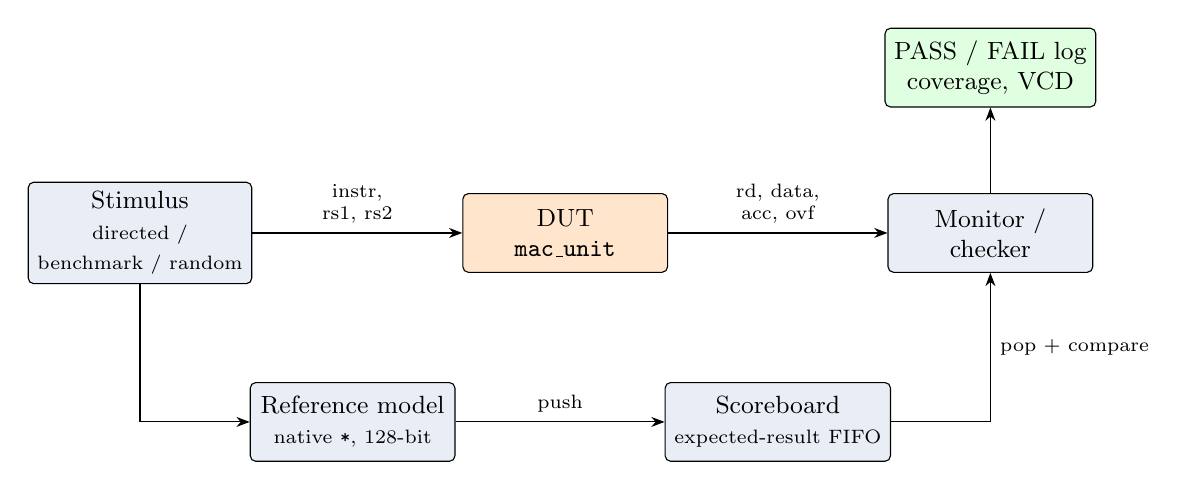
\begin{tikzpicture}[font=\small, >=Stealth,
      blk/.style={draw, fill=accent!10, rounded corners=2pt, minimum height=1.0cm, minimum width=2.6cm, align=center}]
    \node[blk] (stim) at (0,0) {Stimulus\\\scriptsize directed /\\\scriptsize benchmark / random};
    \node[blk, fill=orange!20] (dut) at (5.4,0) {DUT\\\code{mac\_unit}};
    \node[blk] (mon) at (10.8,0) {Monitor /\\checker};
    \node[blk] (model) at (2.7,-2.4) {Reference model\\\scriptsize native \code{*}, 128-bit};
    \node[blk] (sb) at (8.1,-2.4) {Scoreboard\\\scriptsize expected-result FIFO};
    \node[blk, fill=green!12] (rep) at (10.8,2.1) {PASS / FAIL log\\coverage, VCD};
    \draw[->] (stim) -- node[above,font=\scriptsize,align=center]{instr,\\rs1, rs2} (dut);
    \draw[->] (dut) -- node[above,font=\scriptsize,align=center]{rd, data,\\acc, ovf} (mon);
    \draw[->] (stim.south) |- (model.west);
    \draw[->] (model) -- node[above,font=\scriptsize]{push} (sb);
    \draw[->] (sb.east) -| node[right,font=\scriptsize,pos=0.75]{pop + compare} (mon.south);
    \draw[->] (mon) -- (rep);
  \end{tikzpicture}
  \caption{Self-checking testbench architecture.}
  \label{fig:tb}
\end{figure}

\paragraph{Independent reference model.}
The reference model is intentionally implemented in a different way from the
RTL, so that a shared misunderstanding cannot hide a bug. It multiplies with
the simulator's native \code{*} operator instead of Booth recoding, and it
detects saturation by computing a 128-bit sum and comparing it with
INT64\_MAX and INT64\_MIN, instead of using the 65-bit sign-bit XOR.

\paragraph{Checks on every result.}
For each issued instruction the driver calls the model and pushes six expected
values into the scoreboard: \code{rd} index, write enable, illegal flag, rd
data, the 64-bit accumulator and OVF. On every \code{valid\_o}, the monitor
pops one entry and compares all six values, and also checks that exactly two
clock cycles have passed since the instruction was driven.

\paragraph{Analytical golden values.}
The model is not the only reference. The benchmark tests (T6, T10, T11, T12)
also compare the DUT output with values worked out by hand from the
mathematics of the problem.

\section{Test plan}
\begin{table}[H]
  \centering
  \caption{Test plan of the system testbench.}
  \label{tab:testplan}
  \small
  \begin{tabularx}{\linewidth}{@{}clX@{}}
    \toprule
    ID & Test & Purpose / stimulus \\
    \midrule
    T1  & Reset state & Accumulator reads 0 after reset \\
    T2  & Basic arithmetic & \code{mul.acc}, \code{mac}, \code{msu} issued back-to-back \\
    T3  & Sign combinations & $(\pm a)(\pm b)$; sign extension of the high word \\
    T4  & Extreme operands & INT32\_MAX$^2$, INT32\_MIN$^2$, MIN$\cdot$MAX, $(-1)\cdot$MIN$=+2^{31}$ \\
    T5  & Saturation & Positive and negative 64-bit saturation; sticky OVF; clearing \\
    T6  & Unsigned \code{macu} & UINT32\_MAX$^2$, modulo-$2^{64}$ wrap; $\sum_{i=1}^{10} i^2=385$ \\
    T7  & Destination \code{x0} & No write-back, but the accumulator updates \\
    T8  & Illegal instructions & RV32M \code{MUL}, wrong \code{funct7}, \code{NOP} \\
    T9  & Q15 read-out & $0.5\cdot0.5$, $-0.5\cdot0.5$, $-1\cdot-1$ (saturates), $\pm$saturation \\
    T10 & Dot product & $[1..8]\cdot[8..1]=120$; throughput measurement \\
    T11 & Moving-average FIR & 8 taps, step input; analytical ramp response \\
    T12 & Low-pass FIR & Triangular 8-tap filter; DC + Nyquist input \\
    T13 & Constrained random & 3000 instructions, operands biased to corners, $\sim$5\,\% illegal, random bubbles \\
    \bottomrule
  \end{tabularx}
\end{table}

\section{Multiplier unit test}
\code{tb\_booth\_multiplier} instantiates the multiplier twice. The 8-bit
instance is checked \emph{exhaustively} against \code{*} for all
$2^{16}=65{,}536$ operand pairs. The algorithm does not depend on the width,
so this is strong evidence that the recoding logic is correct. The 34-bit
instance, which is the one used in the MAC, is checked on 9 corner cases
(including UINT32\_MAX$^2$ and the 34-bit extremes) and 20{,}000 random pairs.

\section{Constrained-random stimulus}
In T13, each operand is drawn from a biased distribution: 10\,\% each for $0$,
$1$, $-1$, INT32\_MAX and INT32\_MIN, plus small signed values, 16-bit values
and full-range random values. \code{funct3} and \code{rd} are uniformly random.
About 5\,\% of the instructions are deliberately illegal, and about 25\,\% of
the instructions are followed by 1--3 idle cycles, so the test exercises both
back-to-back and gapped issue. A fixed seed makes the regression reproducible.

\section{Mutation test (checking the checker)}
A testbench that never fails proves nothing. To confirm that this one detects
real bugs, a copy of \code{mac\_unit.v} was made with saturation disabled
(\code{sat\_add} hard-wired to the wrapped sum) and simulated with the same
testbench. The testbench reported FAIL on the T5 saturation tests and in the
random regression, as Listing~\ref{lst:mut} shows.

\begin{lstlisting}[style=log, caption={Testbench output for the mutated design (excerpt).}, label={lst:mut}]
  [FAIL]           mac +2^62 -> 2^63 SAT to INT64_MAX
  [FAIL]           mac  (stays saturated, OVF sticky)
  [FAIL]         rdacc.hi               -> 0x7FFFFFFF
  [FAIL]        mac  -> below -2^63, SAT to INT64_MIN
  [FAIL]         rdacc.hi               -> 0x80000000
  [FAIL]                                       random
\end{lstlisting}

\section{System-level verification}
The unit-level testbenches above drive the MAC unit directly. The processor
of Chapter~\ref{ch:cpu} is verified at system level by
\code{tb/tb\_riscv\_soc.v}, which runs complete RISC-V programs: a self-checking
ISA and hazard test (\code{isa\_test}, 18 tests), and four versions of a 16-tap
FIR filter whose 128 outputs are compared bit-exactly against golden values
computed independently in Python.
The testbench also checks the MAC write-back alignment on every MAC
instruction and records a per-cycle pipeline trace. The results are in
Chapter~\ref{ch:sysres}.

%===========================================================================
\chapter{MAC Unit Simulation Results}\label{ch:results}
%===========================================================================

All simulations were run with Icarus Verilog 12 (\code{iverilog -g2005 -Wall},
\code{vvp}). The full terminal log is reproduced in Appendix~\ref{app:log}.

\section{Summary}
\begin{table}[H]
  \centering
  \caption{Verification summary.}
  \label{tab:summary}
  \begin{tabular}{@{}lrrc@{}}
    \toprule
    Testbench & Checks & Errors & Result \\
    \midrule
    \code{tb\_booth\_multiplier} (8-bit exhaustive + 34-bit) & 85{,}545 & 0 & \textbf{PASS} \\
    \code{tb\_mac\_unit} (T1--T13, 3{,}328 instructions)      & 3{,}351  & 0 & \textbf{PASS} \\
    \code{tb\_mac\_unit} on the Yosys gate-level netlist (Ch.~\ref{ch:synth}) & 3{,}351 & 0 & \textbf{PASS} \\
    \bottomrule
  \end{tabular}
\end{table}

\section{Directed test results}
Table~\ref{tab:directed} shows a selection of directed results taken from the
simulation log. Each one matched the reference model on all six compared
fields and on latency.

\begin{table}[H]
  \centering
  \caption{Selected directed test results (DUT output = expected).}
  \label{tab:directed}
  \scriptsize
  \begin{tabular}{@{}cllll@{}}
    \toprule
    Test & Instruction & rd\_data\_o & acc\_o & OVF \\
    \midrule
    T2 & \code{mul.acc 7, 6}        & 42            & \code{0x000000000000002A} & 0 \\
    T2 & \code{mac 3, -4}           & 30            & \code{0x000000000000001E} & 0 \\
    T2 & \code{msu -5, 10}          & 80            & \code{0x0000000000000050} & 0 \\
    T2 & \code{mac 100, 1000}       & 100080        & \code{0x00000000000186F0} & 0 \\
    T3 & \code{mul.acc 12, -13}     & $-156$        & \code{0xFFFFFFFFFFFFFF64} & 0 \\
    T4 & \code{mul.acc MAX, MAX}    & \code{0x00000001} & \code{0x3FFFFFFF00000001} & 0 \\
    T4 & \code{mul.acc MIN, MAX}    & \code{0x80000000} & \code{0xC000000080000000} & 0 \\
    T5 & \code{mac MIN, MIN} (sat.) & \code{0xFFFFFFFF} & \code{0x7FFFFFFFFFFFFFFF} & 1 \\
    T5 & \code{mac MIN, MAX} (sat.) & \code{0x00000000} & \code{0x8000000000000000} & 1 \\
    T5 & \code{mul.acc 2, 3}        & 6             & \code{0x0000000000000006} & 0 \\
    T6 & \code{macu 0xFFFFFFFF$^2$} & \code{0x00000001} & \code{0xFFFFFFFE00000001} & 0 \\
    T6 & \code{macu} (again, wraps) & \code{0x00000002} & \code{0xFFFFFFFC00000002} & 0 \\
    T6 & $\sum_{i=1}^{10}i^2$       & 385           & \code{0x0000000000000181} & 0 \\
    T8 & RV32M \code{MUL} (illegal) & 0, ILLEGAL    & unchanged (\code{0x64}) & 0 \\
    T9 & \code{rdacc.q15} after $0.5\cdot0.5$   & 8192 (0.25)   & \code{0x0000000010000000} & 0 \\
    T9 & \code{rdacc.q15} after $-1\cdot-1$     & 32767 (sat.)  & \code{0x0000000040000000} & 0 \\
    T9 & \code{rdacc.q15} after $\approx -2.0$  & $-32768$ (sat.) & \code{0xFFFFFFFF80010000} & 0 \\
    T10& dot product $[1..8]\cdot[8..1]$       & 120           & \code{0x0000000000000078} & 0 \\
    \bottomrule
  \end{tabular}
\end{table}

\section{Simulation waveforms}
Figures~\ref{fig:wave_t2} and~\ref{fig:wave_t5} were generated from the VCD
dump (\code{sim/mac\_unit.vcd}) produced by the testbench.

In Figure~\ref{fig:wave_t2}, six instructions are issued in consecutive cycles
starting at 80\,ns. The product of each instruction shows up in
\code{s1\_prod} one cycle after issue (42, $-12$, $-50$, 100000), and the
accumulated result shows up on \code{rd\_data\_o}/\code{acc\_o} one cycle
after that (42, 30, 80, 100080). This confirms the two-cycle latency and the
throughput of one instruction per cycle without stalls.

\begin{figure}[H]
  \centering
  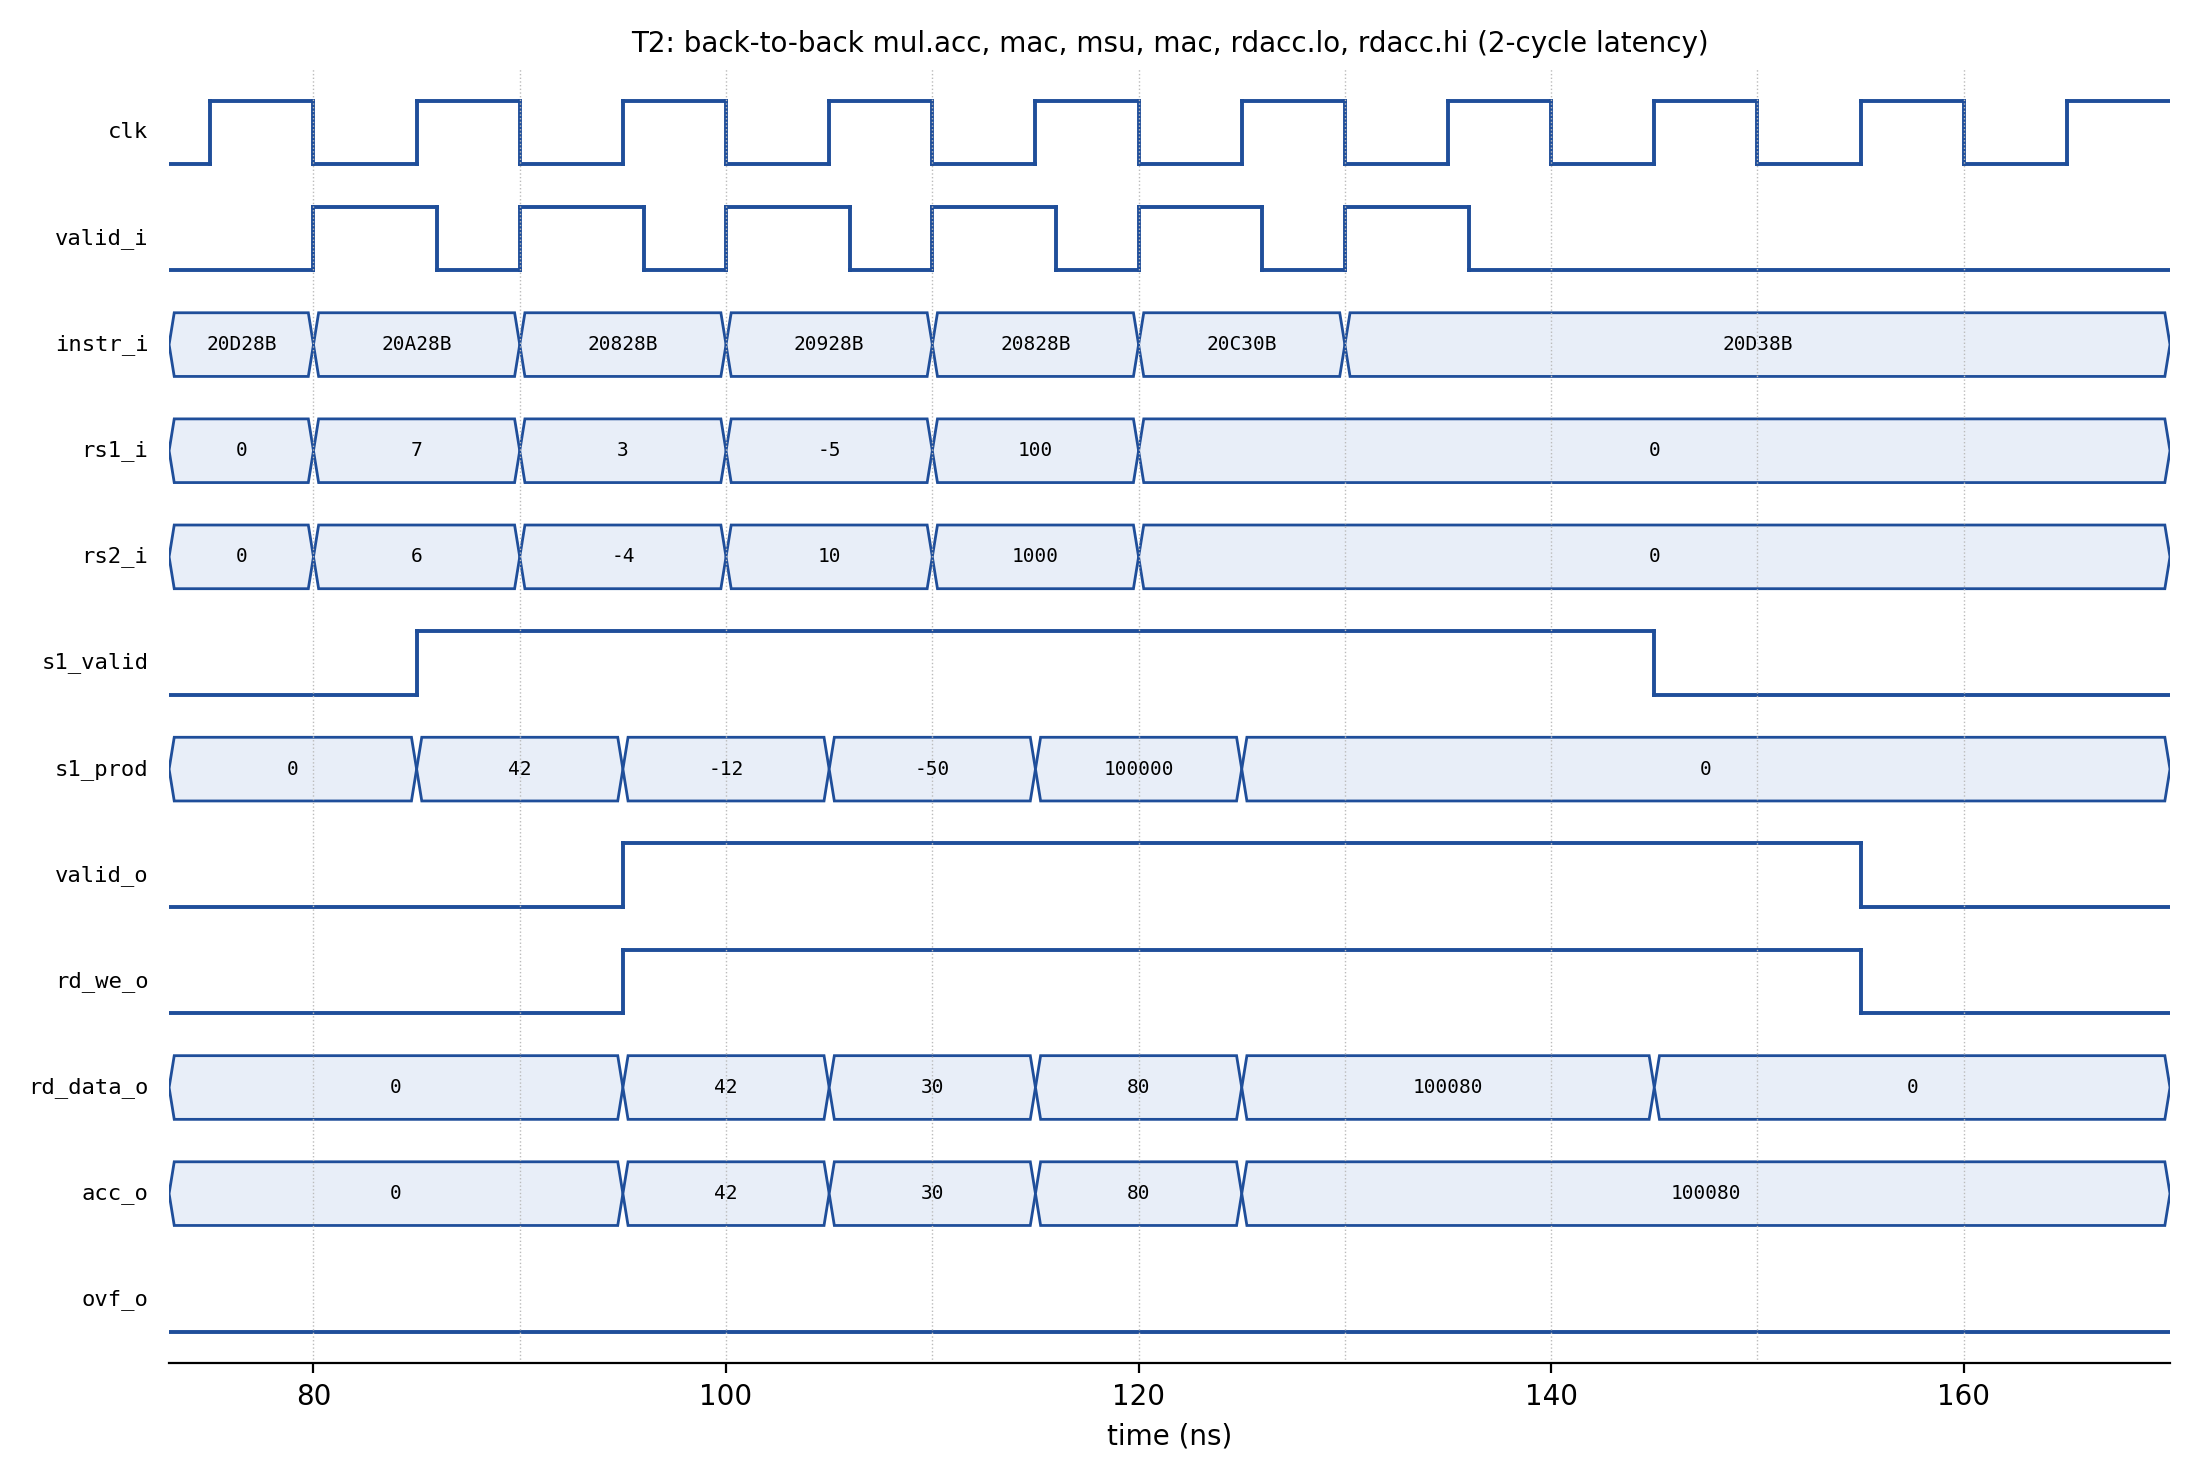
\includegraphics[width=\linewidth]{figures/wave_t2.png}
  \caption{Simulation waveform for T2: back-to-back MAC instructions.}
  \label{fig:wave_t2}
\end{figure}

In Figure~\ref{fig:wave_t5}, \code{mul.acc MIN,MIN} loads $2^{62}$
(\code{0x4000000000000000}). The next \code{mac MIN,MIN} would give $2^{63}$,
which is not representable, so the accumulator saturates to
\code{0x7FFFFFFFFFFFFFFF} and \code{ovf\_o} goes high. It stays high during
the following \code{mac} and \code{rdacc.hi}, and is cleared by
\code{clracc} at 415\,ns.

\begin{figure}[H]
  \centering
  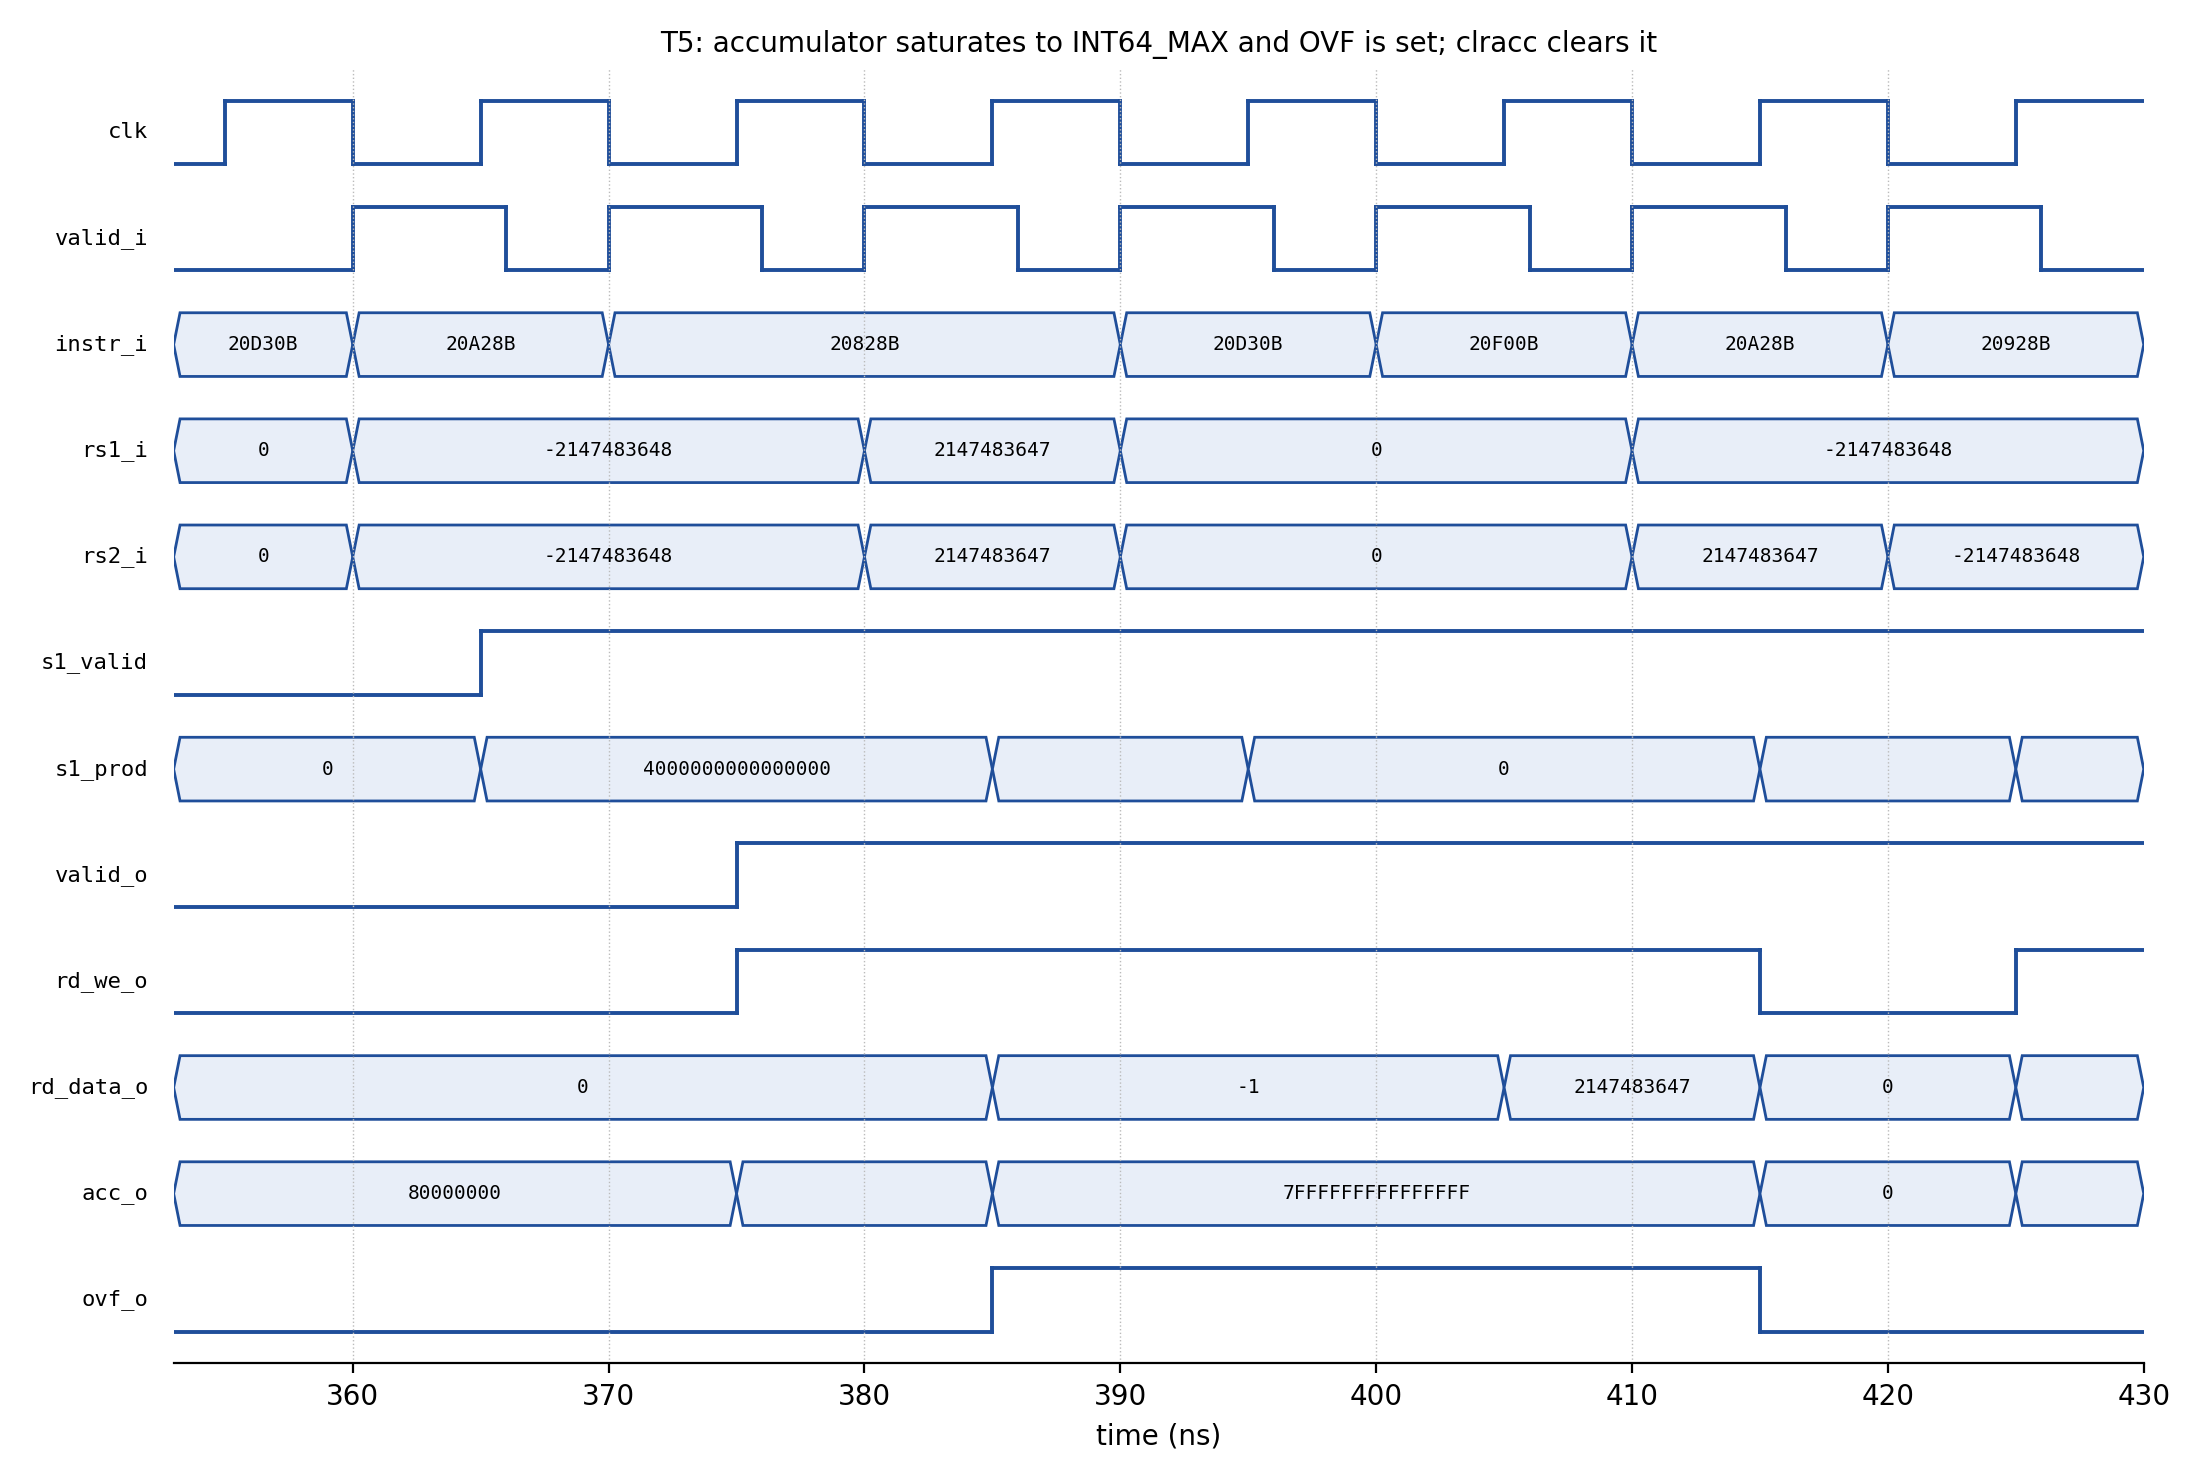
\includegraphics[width=\linewidth]{figures/wave_t5.png}
  \caption{Simulation waveform for T5: positive saturation and the sticky overflow flag.}
  \label{fig:wave_t5}
\end{figure}

\section{DSP benchmark 1: moving-average FIR}
An 8-tap moving-average filter with $h[k]=4096$ (0.125 in Q15) is driven by
a step of amplitude $16384$ (0.5). The analytical output is
$y[n]=2048(n+1)$ for $n<8$ and $16384$ afterwards. Each output sample is
computed by the instruction sequence \code{mul.acc}, seven \code{mac}, and
\code{rdacc.q15}. All 12 DUT outputs exactly match the analytical values
(Table~\ref{tab:ma}, Figure~\ref{fig:fir}a).

\begin{table}[H]
  \centering
  \caption{Moving-average FIR step response.}
  \label{tab:ma}
  \small
  \begin{tabular}{@{}lrrrrrrrrr@{}}
    \toprule
    $n$ & 0 & 1 & 2 & 3 & 4 & 5 & 6 & 7 & 8--11 \\
    \midrule
    DUT $y[n]$  & 2048 & 4096 & 6144 & 8192 & 10240 & 12288 & 14336 & 16384 & 16384 \\
    Analytical  & 2048 & 4096 & 6144 & 8192 & 10240 & 12288 & 14336 & 16384 & 16384 \\
    \bottomrule
  \end{tabular}
\end{table}

\section{DSP benchmark 2: triangular low-pass FIR}
The symmetric filter
$h=\{1024,3072,5120,7168,7168,5120,3072,1024\}$ has a DC gain of
$\sum h[k]/2^{15}=1$. Its gain at the Nyquist frequency is zero:
\begin{equation}
  H(e^{j\pi}) = \sum_k h[k](-1)^k
  = 1024-3072+5120-7168+7168-5120+3072-1024 = 0.
\end{equation}
The input $x[n]=8000+6000(-1)^n$, a DC level plus a Nyquist-frequency tone,
must therefore give exactly $y[n]=8000$ once the 8-sample window is full
($n\ge7$). The DUT produces exactly 8000 for every steady-state sample: all
9 checks pass (Table~\ref{tab:lpf}, Figure~\ref{fig:fir}b). The tone is
removed completely.

\begin{table}[H]
  \centering
  \caption{Low-pass FIR response to DC + Nyquist input.}
  \label{tab:lpf}
  \small
  \begin{tabular}{@{}lrrrrrrrrr@{}}
    \toprule
    $n$ & 0 & 1 & 2 & 3 & 4 & 5 & 6 & 7 & 8--15 \\
    \midrule
    $x[n]$      & 14000 & 2000 & 14000 & 2000 & 14000 & 2000 & 14000 & 2000 & alt. \\
    DUT $y[n]$  & 437 & 1375 & 2812 & 4750 & 6312 & 7375 & 7937 & \textbf{8000} & \textbf{8000} \\
    \bottomrule
  \end{tabular}
\end{table}

\begin{figure}[H]
  \centering
  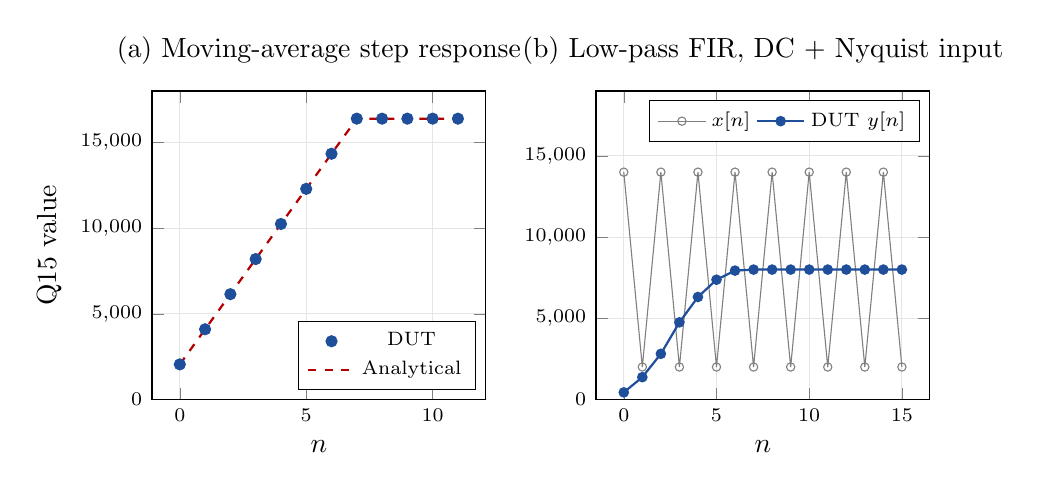
\begin{tikzpicture}
    \begin{axis}[
        name=ma, width=0.48\linewidth, height=5.5cm,
        title={(a) Moving-average step response},
        xlabel={$n$}, ylabel={Q15 value}, ymin=0, ymax=18000,
        legend pos=south east, legend style={font=\scriptsize},
        grid=major, grid style={gray!20}, tick label style={font=\scriptsize}, scaled y ticks=false]
      \addplot[only marks, mark=*, accent] coordinates {
        (0,2048)(1,4096)(2,6144)(3,8192)(4,10240)(5,12288)
        (6,14336)(7,16384)(8,16384)(9,16384)(10,16384)(11,16384)};
      \addlegendentry{DUT}
      \addplot[thick, red!70!black, dashed, domain=0:11, samples=12]
        {x<8 ? 2048*(x+1) : 16384};
      \addlegendentry{Analytical}
    \end{axis}
    \begin{axis}[
        at={(ma.east)}, anchor=west, xshift=1.4cm,
        width=0.48\linewidth, height=5.5cm,
        title={(b) Low-pass FIR, DC + Nyquist input},
        xlabel={$n$}, ymin=0, ymax=19000,
        legend pos=north east, legend columns=2, legend style={font=\scriptsize},
        grid=major, grid style={gray!20}, tick label style={font=\scriptsize}, scaled y ticks=false]
      \addplot[gray, mark=o, mark size=1.5pt] coordinates {
        (0,14000)(1,2000)(2,14000)(3,2000)(4,14000)(5,2000)(6,14000)(7,2000)
        (8,14000)(9,2000)(10,14000)(11,2000)(12,14000)(13,2000)(14,14000)(15,2000)};
      \addlegendentry{$x[n]$}
      \addplot[thick, accent, mark=*, mark size=1.5pt] coordinates {
        (0,437)(1,1375)(2,2812)(3,4750)(4,6312)(5,7375)(6,7937)(7,8000)
        (8,8000)(9,8000)(10,8000)(11,8000)(12,8000)(13,8000)(14,8000)(15,8000)};
      \addlegendentry{DUT $y[n]$}
    \end{axis}
  \end{tikzpicture}
  \caption{FIR benchmark results computed by the MAC unit.}
  \label{fig:fir}
\end{figure}

\section{Functional coverage}
\begin{table}[H]
  \centering
  \caption{Functional coverage collected over the full regression.}
  \label{tab:cov}
  \small
  \begin{tabular}{@{}lr@{\qquad}lr@{}}
    \toprule
    Coverage item & Count & Coverage item & Count \\
    \midrule
    \code{mac}       & 570 & \code{rdacc.hi}   & 386 \\
    \code{msu}       & 338 & \code{rdacc.q15}  & 393 \\
    \code{mul.acc}   & 378 & \code{clracc}     & 374 \\
    \code{macu}      & 381 & Illegal instructions & 162 \\
    \code{rdacc.lo}  & 346 & Saturation events & 7 (+ directed) \\
    \code{rd = x0}   & 360 & Idle-gap insertions & 684 \\
    \bottomrule
  \end{tabular}
\end{table}

Every instruction, the illegal-instruction path, saturation in both directions,
\code{x0} suppression, and both back-to-back and gapped issue were exercised
many times.

\section{Performance analysis}
\paragraph{Measured.}
In T10, nine instructions (eight multiply-accumulates and one read) were issued
in nine consecutive cycles, i.e. one instruction per cycle. An $N$-tap FIR
therefore costs $N+1$ MAC-unit instructions per output sample: 9 for the
8-tap filters in this report.

\paragraph{Comparison with RV32IM (instruction count estimate).}
On a base RV32IM core, adding a full 32$\times$32-bit signed product into a
64-bit sum requires \code{mul} (low word), \code{mulh} (high word), \code{add}
(low), \code{sltu} (carry), \code{add} (high) and \code{add} (carry): six
instructions, with no saturation. The \code{mac} instruction does the same
work, plus saturation, in one instruction. Table~\ref{tab:perf} compares the
two for one output of an 8-tap FIR. These figures count only the arithmetic
instructions and exclude loads and loop overhead, which are the same for both.
Chapter~\ref{ch:sysres} replaces this estimate with \emph{measured} cycle
counts from complete programs running on the 5-stage processor.

\begin{table}[H]
  \centering
  \caption{Arithmetic instruction count per output of an 8-tap FIR (estimate).}
  \label{tab:perf}
  \small
  \begin{tabular}{@{}lccc@{}}
    \toprule
    Implementation & Per tap & Per output (8 taps) & Saturation \\
    \midrule
    RV32IM, 64-bit accumulation        & 6 & 48 + conversion & no \\
    RV32IM, 32-bit accumulation (Q15 only) & 2 & 16 + conversion & no \\
    This MAC unit                      & 1 & 8 + 1 (\code{rdacc.q15}) & yes \\
    \bottomrule
  \end{tabular}
\end{table}

%===========================================================================
\chapter{System-Level Simulation Results}\label{ch:sysres}
%===========================================================================

The processor was simulated in Icarus Verilog with the system testbench
\code{tb/tb\_riscv\_soc.v}. For each program, the testbench loads the program
and data images and runs the core until ECALL. It then checks that
\code{a0}~$=$~\code{0x600D}, the success code of the self-checking programs,
and compares every output sample with the golden file, bit by bit. In
addition, on every MAC write-back it checks that the MAC unit's
\code{valid\_o}/\code{rd\_addr\_o} line up with the core's MEM/WB register.
Finally, it reports the core's hardware performance counters, writes a
per-cycle pipeline trace (CSV) and, optionally, a VCD waveform. The whole flow
(build, compile, run, collect) is automated by \code{sw/run\_cpu\_sims.py}.

\section{Results summary}
\begin{table}[H]
  \centering
  \caption{Programs executed on the 5-stage core (all results from the hardware performance counters).}
  \label{tab:cpures}
  \small
  \begin{tabular}{@{}lcrrrrrr@{}}
    \toprule
    Program & Result & Cycles & Instr. & CPI & Stalls & Flushes & MAC instr. \\
    \midrule
    \code{isa\_test}            & \textbf{PASS} &    348 &    300 & 1.160 & 8 &   18 &    22 \\
    \code{fir\_mac\_loop}       & \textbf{PASS} & 19{,}724 & 15{,}626 & 1.262 & 0 & 2{,}047 & 2{,}304 \\
    \code{fir\_rv32im\_loop}    & \textbf{PASS} & 31{,}363 & 26{,}895 & 1.166 & 0 & 2{,}232 &     0 \\
    \code{fir\_mac\_unrolled}   & \textbf{PASS} &  7{,}180 &  6{,}922 & 1.037 & 0 &  127 & 2{,}176 \\
    \code{fir\_rv32im\_unrolled}& \textbf{PASS} & 19{,}203 & 18{,}575 & 1.034 & 0 &  312 &     0 \\
    \bottomrule
  \end{tabular}
\end{table}

The \code{isa\_test} program passed all 18 self-checks (\code{a0 = 0x600D}).
Its 8 stall cycles are the deliberate load-use and MAC-use hazards in tests
T7, T8, T12, T13 and T14, and every one was resolved correctly. All four FIR
programs produced \textbf{128/128 output samples bit-identical} to the golden
model, and no MAC write-back was ever misaligned with the core pipeline.

\paragraph{Mutation testing of the processor.}
To show that the system tests can find real pipeline bugs, two faulty copies
of the core were simulated with the same programs (Table~\ref{tab:cpumut}).
Both bugs are caught by \code{isa\_test}. The FIR programs still pass,
because they were scheduled to avoid hazards, which is exactly why a
dedicated ISA/hazard test is needed in addition to application benchmarks.

\begin{table}[H]
  \centering
  \caption{Processor mutation tests.}
  \label{tab:cpumut}
  \small
  \begin{tabularx}{\linewidth}{@{}Xll@{}}
    \toprule
    Injected fault & \code{isa\_test} & \code{fir\_mac\_loop} \\
    \midrule
    WB$\rightarrow$EX forwarding of operand A disabled & \textbf{FAIL} at T1 (\code{a0}=1) & pass \\
    Load-use / MAC-use stall disabled                  & \textbf{FAIL} at T7 (\code{a0}=7) & pass \\
    \bottomrule
  \end{tabularx}
\end{table}

\section{Pipeline behaviour}\label{sec:pipeviz}
The pipeline diagrams below were \emph{reconstructed from the simulation
trace}, not drawn by hand. Each row is one dynamic instruction; each column is
one clock cycle. Colours mark the stage the instruction occupies; orange
MAC1/MAC2 cells show MAC instructions in the MAC unit's two stages; hatched
cells are stall cycles; \emph{fwd} marks operands forwarded from MEM or WB;
grey rows are wrong-path instructions squashed by a taken branch.

\begin{figure}[H]
  \centering
  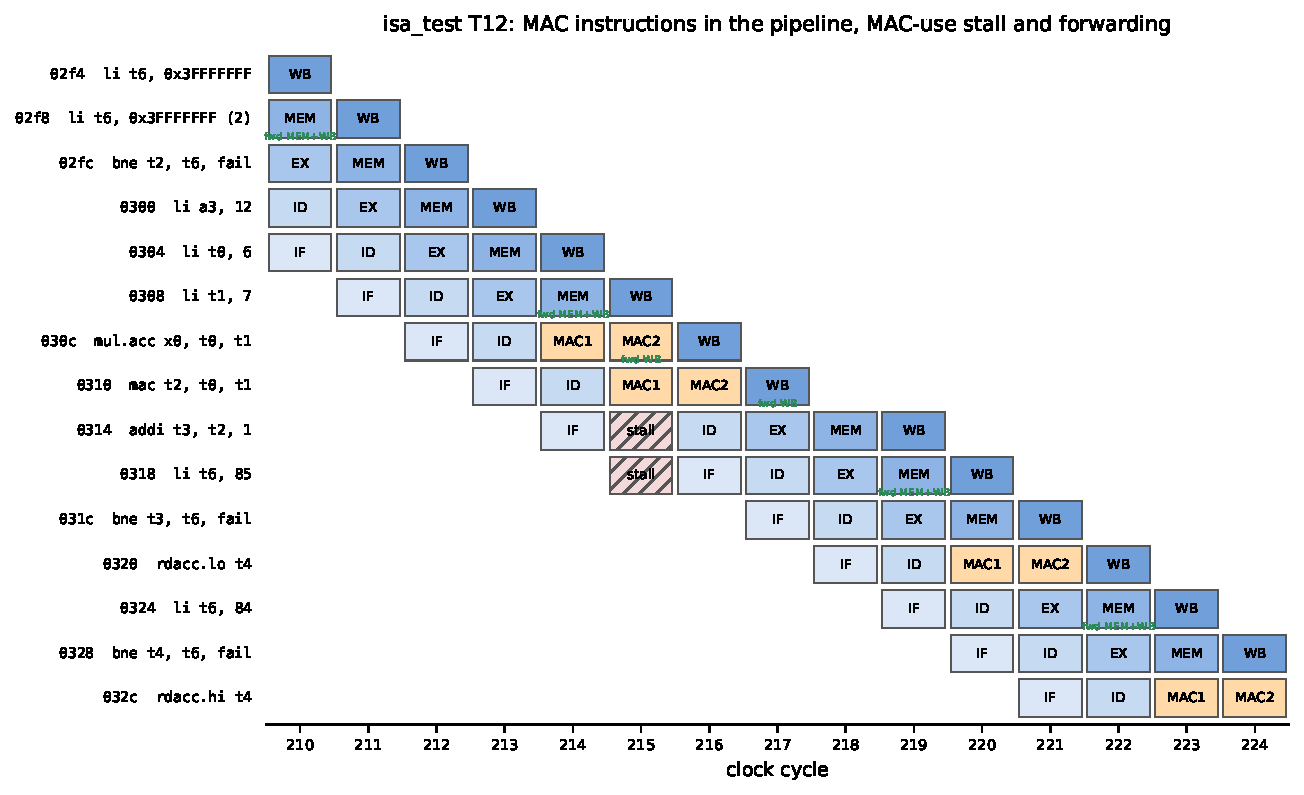
\includegraphics[width=\linewidth]{figures/pipe_isa_mac_hazard.pdf}
  \caption{\code{isa\_test} T12 executing: \code{mul.acc}, \code{mac} and the
    dependent \code{addi t3,t2,1}. The \code{addi} is held in ID for one cycle
    (MAC-use stall) and then receives \code{t2} from WB; the result is 85 as
    expected.}
  \label{fig:pipe_isa}
\end{figure}

In Figure~\ref{fig:pipe_isa}, \code{mul.acc} and \code{mac} occupy MAC1/MAC2
in consecutive cycles without any interference, because the accumulator is
read and written only in MAC stage~2. The instruction that consumes the MAC
result is stalled once by the hazard unit and then gets the value forwarded
from WB. This is exactly the behaviour designed in Chapter~\ref{ch:cpu}.

\begin{figure}[H]
  \centering
  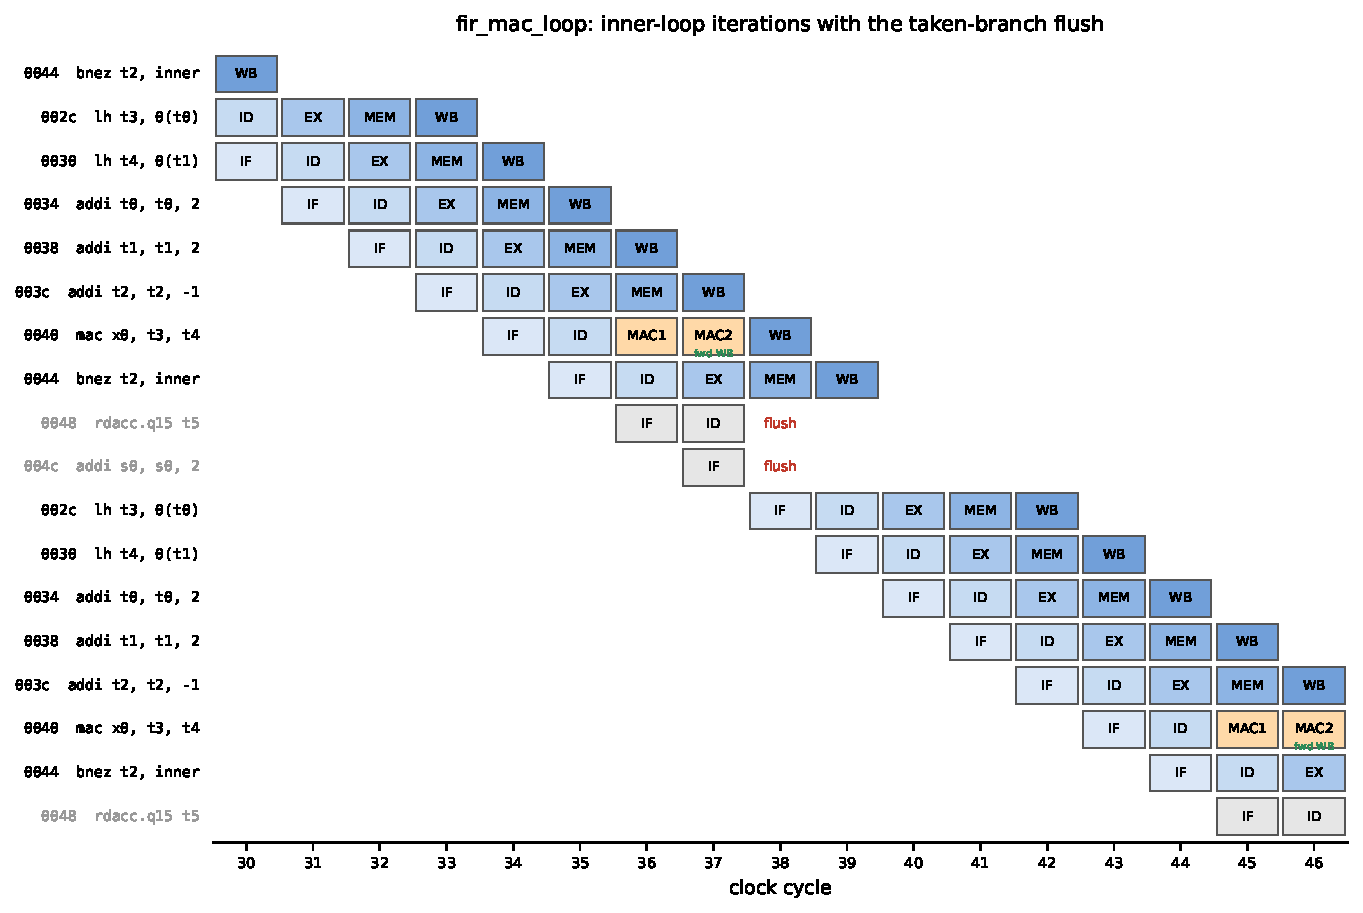
\includegraphics[width=\linewidth]{figures/pipe_fir_loop.pdf}
  \caption{\code{fir\_mac\_loop}: two iterations of the inner loop. Every
    iteration ends with a taken \code{bnez}, which squashes the two
    instructions fetched behind it (2-cycle penalty).}
  \label{fig:pipe_fir}
\end{figure}

\begin{figure}[H]
  \centering
  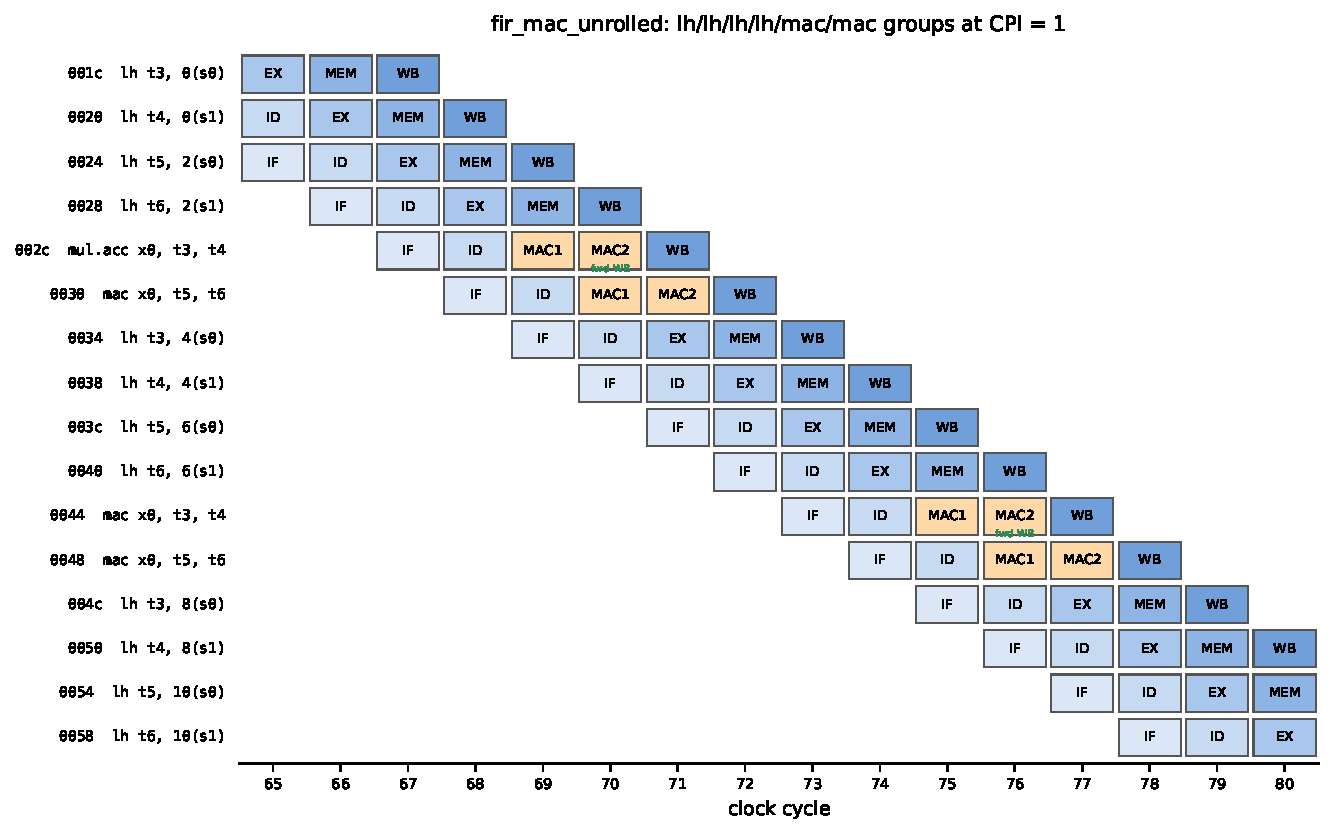
\includegraphics[width=\linewidth]{figures/pipe_fir_unrolled.pdf}
  \caption{\code{fir\_mac\_unrolled}: the unrolled \code{lh}/\code{lh}/\code{lh}/\code{lh}/\code{mac}/\code{mac}
    pattern issues one instruction per cycle with no stalls or flushes.}
  \label{fig:pipe_unrolled}
\end{figure}

Figure~\ref{fig:pipe_fir} explains why the looped FIR has a CPI of 1.26: the
taken branch at the end of each 7-instruction iteration wastes 2 of every
9 cycles. Unrolling (Figure~\ref{fig:pipe_unrolled}) removes the branches
from the tap loop. The pipeline then reaches CPI~1.037, and the MAC unit
receives a new operand pair every third cycle (\code{lh}, \code{lh},
\code{mac}).

\section{Processor waveform}
Figure~\ref{fig:wave_cpu} shows the VCD waveform of \code{fir\_mac\_loop}
around the end of output sample $y[2]$. The first five rows show which
instruction is in each pipeline stage. Note the bubbles after the taken
\code{bnez} and the \code{mac} moving from EX to MEM to WB. The orange rows
show the MAC unit itself. The \code{valid\_i} signal is high while a \code{mac}
is in EX, and its operands $x[n]$ and $h[k]$ (for example $-2708$ and $-114$)
arrive through the forwarding network. One cycle later, the Booth product
appears in \code{s1\_prod} ($-2708\times-114 = 308{,}712$), and one cycle after
that the accumulator updates ($-1{,}731{,}669 + 308{,}712 = -1{,}422{,}957$).
After the loop exits, \code{rdacc.q15} writes
$\lfloor -1{,}422{,}957 / 2^{15}\rfloor = -44$ to register \code{t5} (x30),
and the following \code{sh} stores it as $y[2]$. This value matches the
golden model.

\begin{landscape}
\begin{figure}[p]
  \centering
  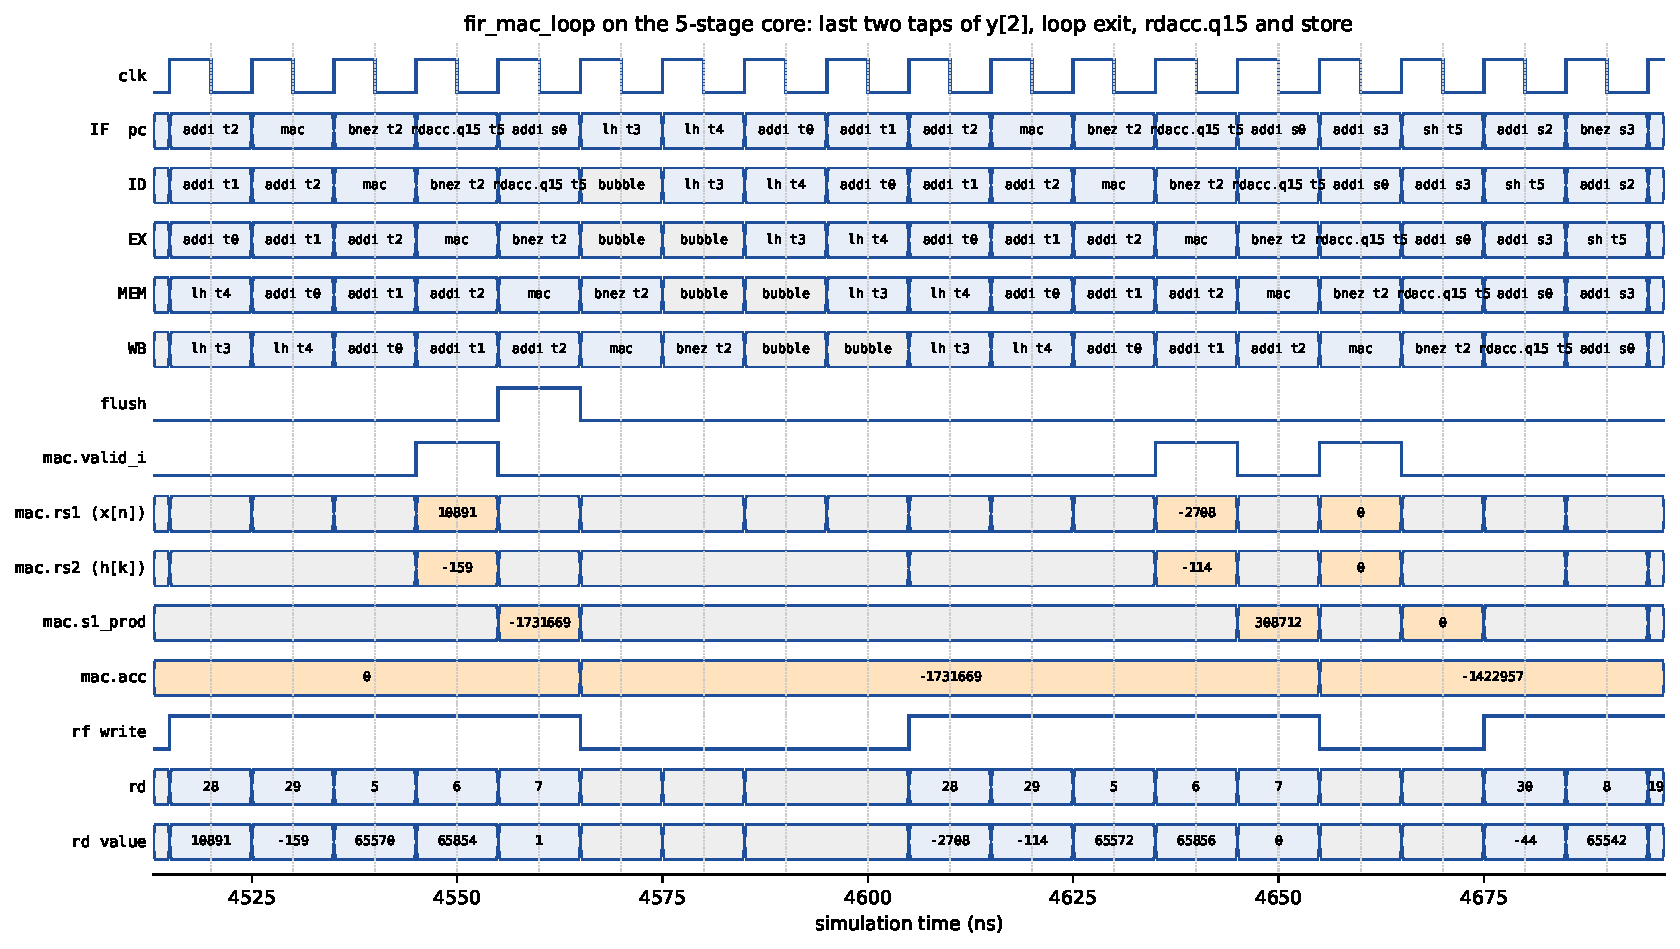
\includegraphics[width=\linewidth]{figures/wave_cpu_mac.pdf}
  \caption[Simulation waveform of the 5-stage core executing the FIR program]{Simulation waveform of the 5-stage core executing \code{fir\_mac\_loop}
    (from \code{sim/cpu/fir\_mac\_loop.vcd}). Pipeline-stage rows show the
    instruction in each stage (grey = bubble); orange rows are MAC-unit
    signals; bus values are blanked while their valid signal is low.}
  \label{fig:wave_cpu}
\end{figure}
\end{landscape}

\section{DSP results: the FIR filter on the processor}
Figure~\ref{fig:fir_time} shows the input signal and the output that the
processor computed with the MAC instructions. The high-frequency tone is
removed and the wanted tone passes through, delayed by the filter's group
delay of 7.5 samples. The lower panel shows two error curves. The difference
from the golden model is \textbf{exactly zero} for all 128 samples, while the
difference from an ideal floating-point filter is at most 2.5\,LSB (1.2\,LSB
rms), which is just the Q15 quantisation of the taps and the signal.

\begin{figure}[H]
  \centering
  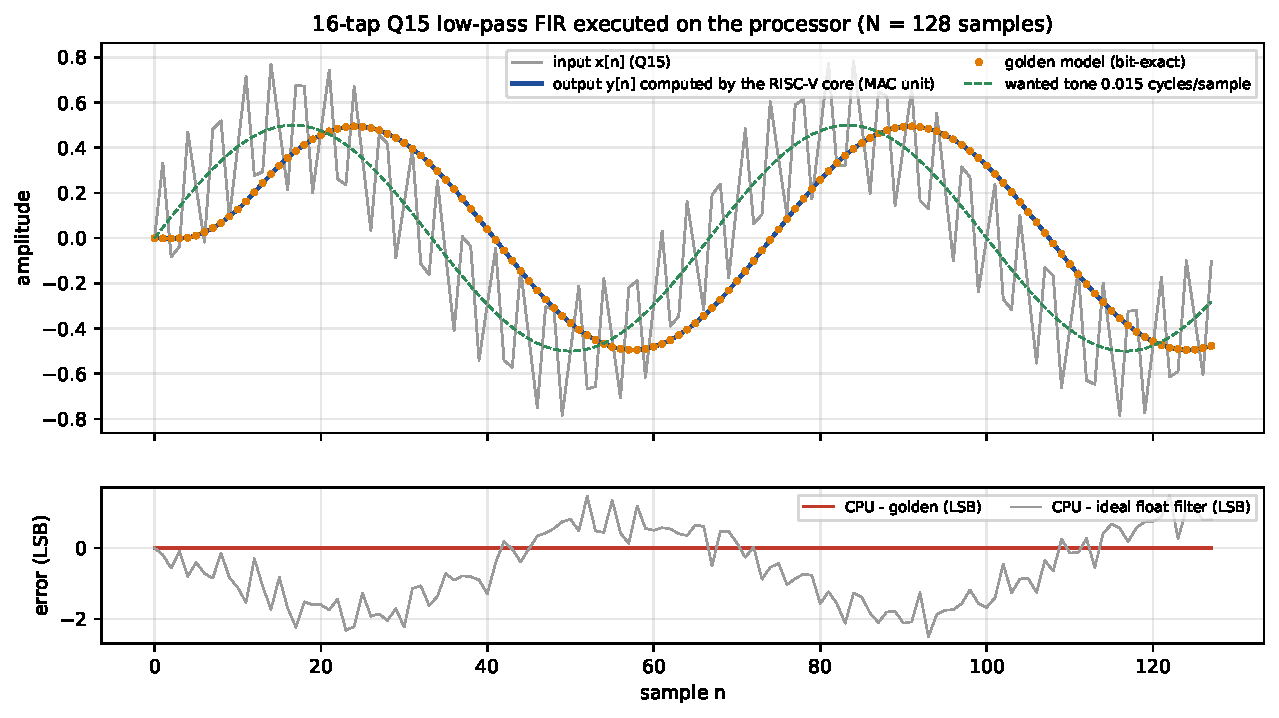
\includegraphics[width=\linewidth]{figures/fir_time.pdf}
  \caption{FIR filtering executed on the RISC-V core: input, CPU output and
    golden model (top), and the error against the golden model and against
    an ideal floating-point filter (bottom).}
  \label{fig:fir_time}
\end{figure}

The spectra in Figure~\ref{fig:fir_spec} quantify the result. The unwanted
tone at 0.3 cycles/sample drops from $-11.3$\,dBFS to $-71.4$\,dBFS, an
attenuation of \textbf{60.1\,dB}, which agrees with the filter's theoretical
response $|H(0.3)| = -60.2$\,dB (Figure~\ref{fig:fir_h}). The wanted tone at
0.015 cycles/sample, by contrast, changes by only $-0.1$\,dB.

\begin{figure}[H]
  \centering
  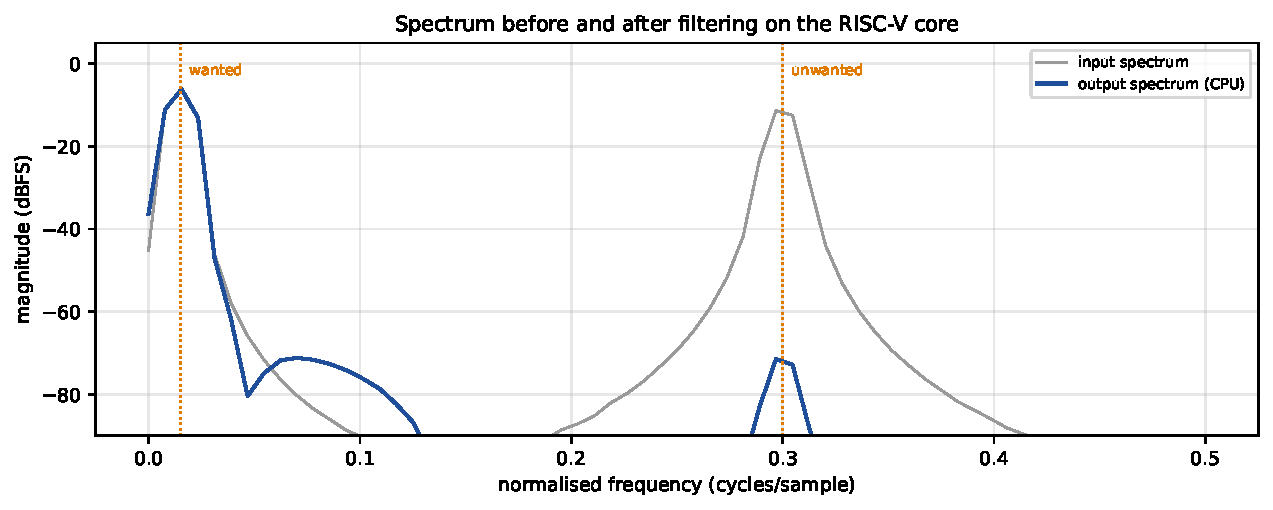
\includegraphics[width=\linewidth]{figures/fir_spectrum.pdf}
  \caption{Spectrum of the input and of the output computed by the processor.}
  \label{fig:fir_spec}
\end{figure}

\begin{figure}[H]
  \centering
  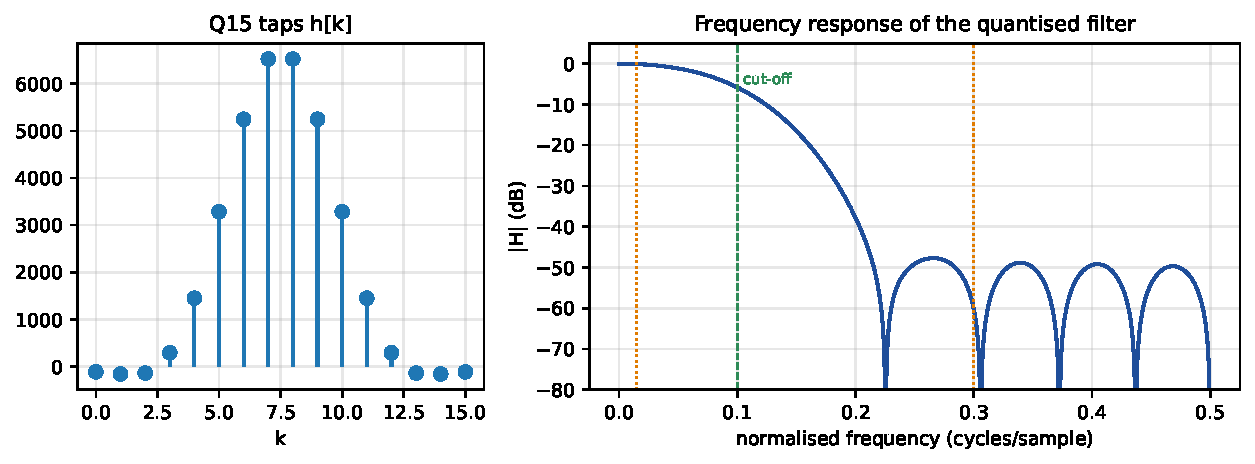
\includegraphics[width=\linewidth]{figures/fir_freqresp.pdf}
  \caption{Quantised Q15 filter taps and frequency response.}
  \label{fig:fir_h}
\end{figure}

\section{Performance: MAC unit vs.\ plain RV32IM}
Because both versions of the filter run on the same core and produce the same
bit-exact output, their cycle counts can be compared directly
(Figure~\ref{fig:perf}, Table~\ref{tab:speedup}).

\begin{figure}[H]
  \centering
  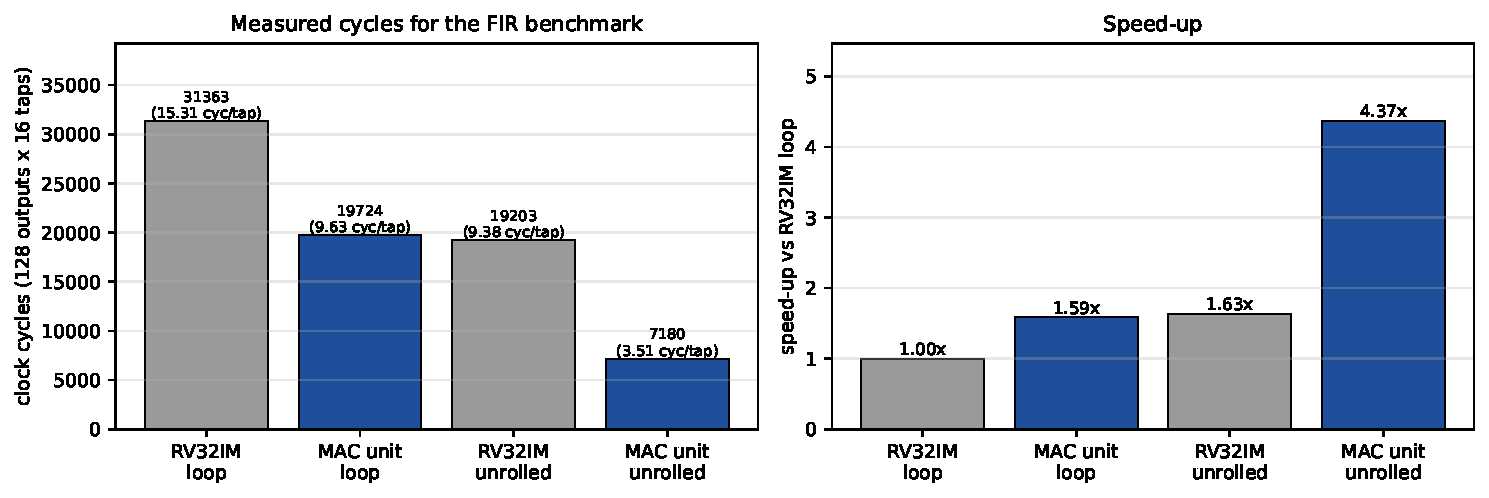
\includegraphics[width=\linewidth]{figures/perf_cycles.pdf}
  \caption{Measured FIR execution time (128 outputs $\times$ 16 taps) and speed-up.}
  \label{fig:perf}
\end{figure}

\begin{table}[H]
  \centering
  \caption{FIR benchmark: MAC instructions vs.\ RV32IM software (measured).}
  \label{tab:speedup}
  \small
  \begin{tabular}{@{}lrrrrr@{}}
    \toprule
    Version & Cycles & Cycles/tap & Instructions & Code size & Speed-up \\
    \midrule
    RV32IM loop             & 31{,}363 & 15.31 & 26{,}895 &  51 instr. & 1.00$\times$ \\
    MAC loop                & 19{,}724 &  9.63 & 15{,}626 &  27 instr. & \textbf{1.59$\times$} \\
    RV32IM unrolled         & 19{,}203 &  9.38 & 18{,}575 & 166 instr. & 1.63$\times$ \\
    MAC unrolled            &  7{,}180 &  3.51 &  6{,}922 &  64 instr. & \textbf{4.37$\times$} \\
    \midrule
    MAC vs.\ RV32IM, same code style & \multicolumn{5}{l}{loop: \textbf{1.59$\times$} faster;\quad unrolled: \textbf{2.67$\times$} faster, 2.6$\times$ smaller code} \\
    \bottomrule
  \end{tabular}
\end{table}

Figure~\ref{fig:breakdown} shows where the cycles go, measured with the
performance counters. With the unrolled MAC code, 96\,\% of all cycles retire
a useful instruction, whereas in the looped versions 14--21\,\% of the cycles
are lost to branch flushes. The scheduled FIR code, on the other hand, has no
load-use or MAC-use stalls at all.
At the processor's post-route clock frequency of 34.6\,MHz on the ECP5 FPGA
(Chapter~\ref{ch:synth}), the unrolled MAC version filters one output sample
in 56~cycles (1.6\,$\mu$s, about 616{,}000 samples/s). The unrolled RV32IM
version needs 150~cycles (4.3\,$\mu$s).

\begin{figure}[H]
  \centering
  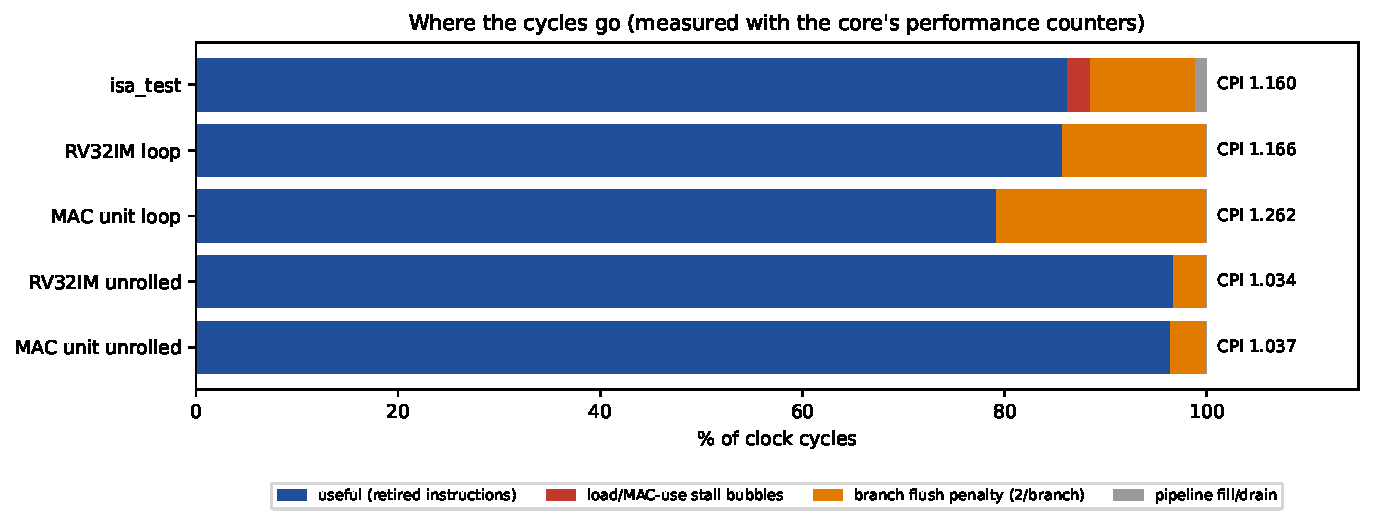
\includegraphics[width=\linewidth]{figures/perf_breakdown.pdf}
  \caption{Cycle breakdown and CPI of every program.}
  \label{fig:breakdown}
\end{figure}

%===========================================================================
\chapter{Logic Synthesis and FPGA Implementation}\label{ch:synth}
%===========================================================================

The RTL was synthesised with the open-source \textbf{Yosys 0.70} synthesis
suite~\cite{yosys} and placed and routed with \textbf{nextpnr-ecp5}~\cite{nextpnr}.
Four flows were used (scripts in Appendix~\ref{app:synth}). The first flow
produces the RTL schematics: Yosys elaborates the design, and
netlistsvg~\cite{netlistsvg} draws the resulting netlist. The second flow is
generic (ASIC-style) gate-level synthesis, in which technology mapping with
ABC targets 2-input gates and D flip-flops, applied both to the MAC unit and
to the complete processor. The third flow is FPGA implementation on a Lattice
ECP5 LFE5U-85F (\code{synth\_ecp5} + nextpnr place \& route, speed grade~6),
carried out for the MAC unit with the Booth multiplier, for the MAC unit with
hard DSP multipliers as a comparison, and for the complete RV32IM core with
the MAC unit. The fourth flow is post-synthesis gate-level simulation of the
synthesised netlist.

\section{RTL schematics generated by Yosys}
Figure~\ref{fig:sch_booth} shows the radix-4 Booth multiplier as Yosys
elaborates it. A small instance ($W=6$) is used so that the structure stays
readable. Each of the three 3-bit groups of $B$ is decoded by \code{\$eq}
comparators that drive a Booth-recoding multiplexer (\code{\$pmux}) choosing
$0,\pm A,\pm 2A$. Yosys then merged the weighted partial-product additions
into multiply-accumulate (\code{\$macc}) and adder (\code{\$alu}) cells,
exactly as described in Table~\ref{tab:booth}. Figure~\ref{fig:sch_booth_g}
shows the same circuit after technology mapping: 216 two-input gates.
Figure~\ref{fig:sch_mac} shows the complete \code{mac\_unit}: the Booth
multiplier appears as one block, surrounded by the decoder, the stage-1 and
stage-2 registers (\code{\$dff}/\code{\$sdff}), the 65-bit adder and
subtractor, the saturation comparators and the result multiplexers.

\begin{figure}[H]
  \centering
  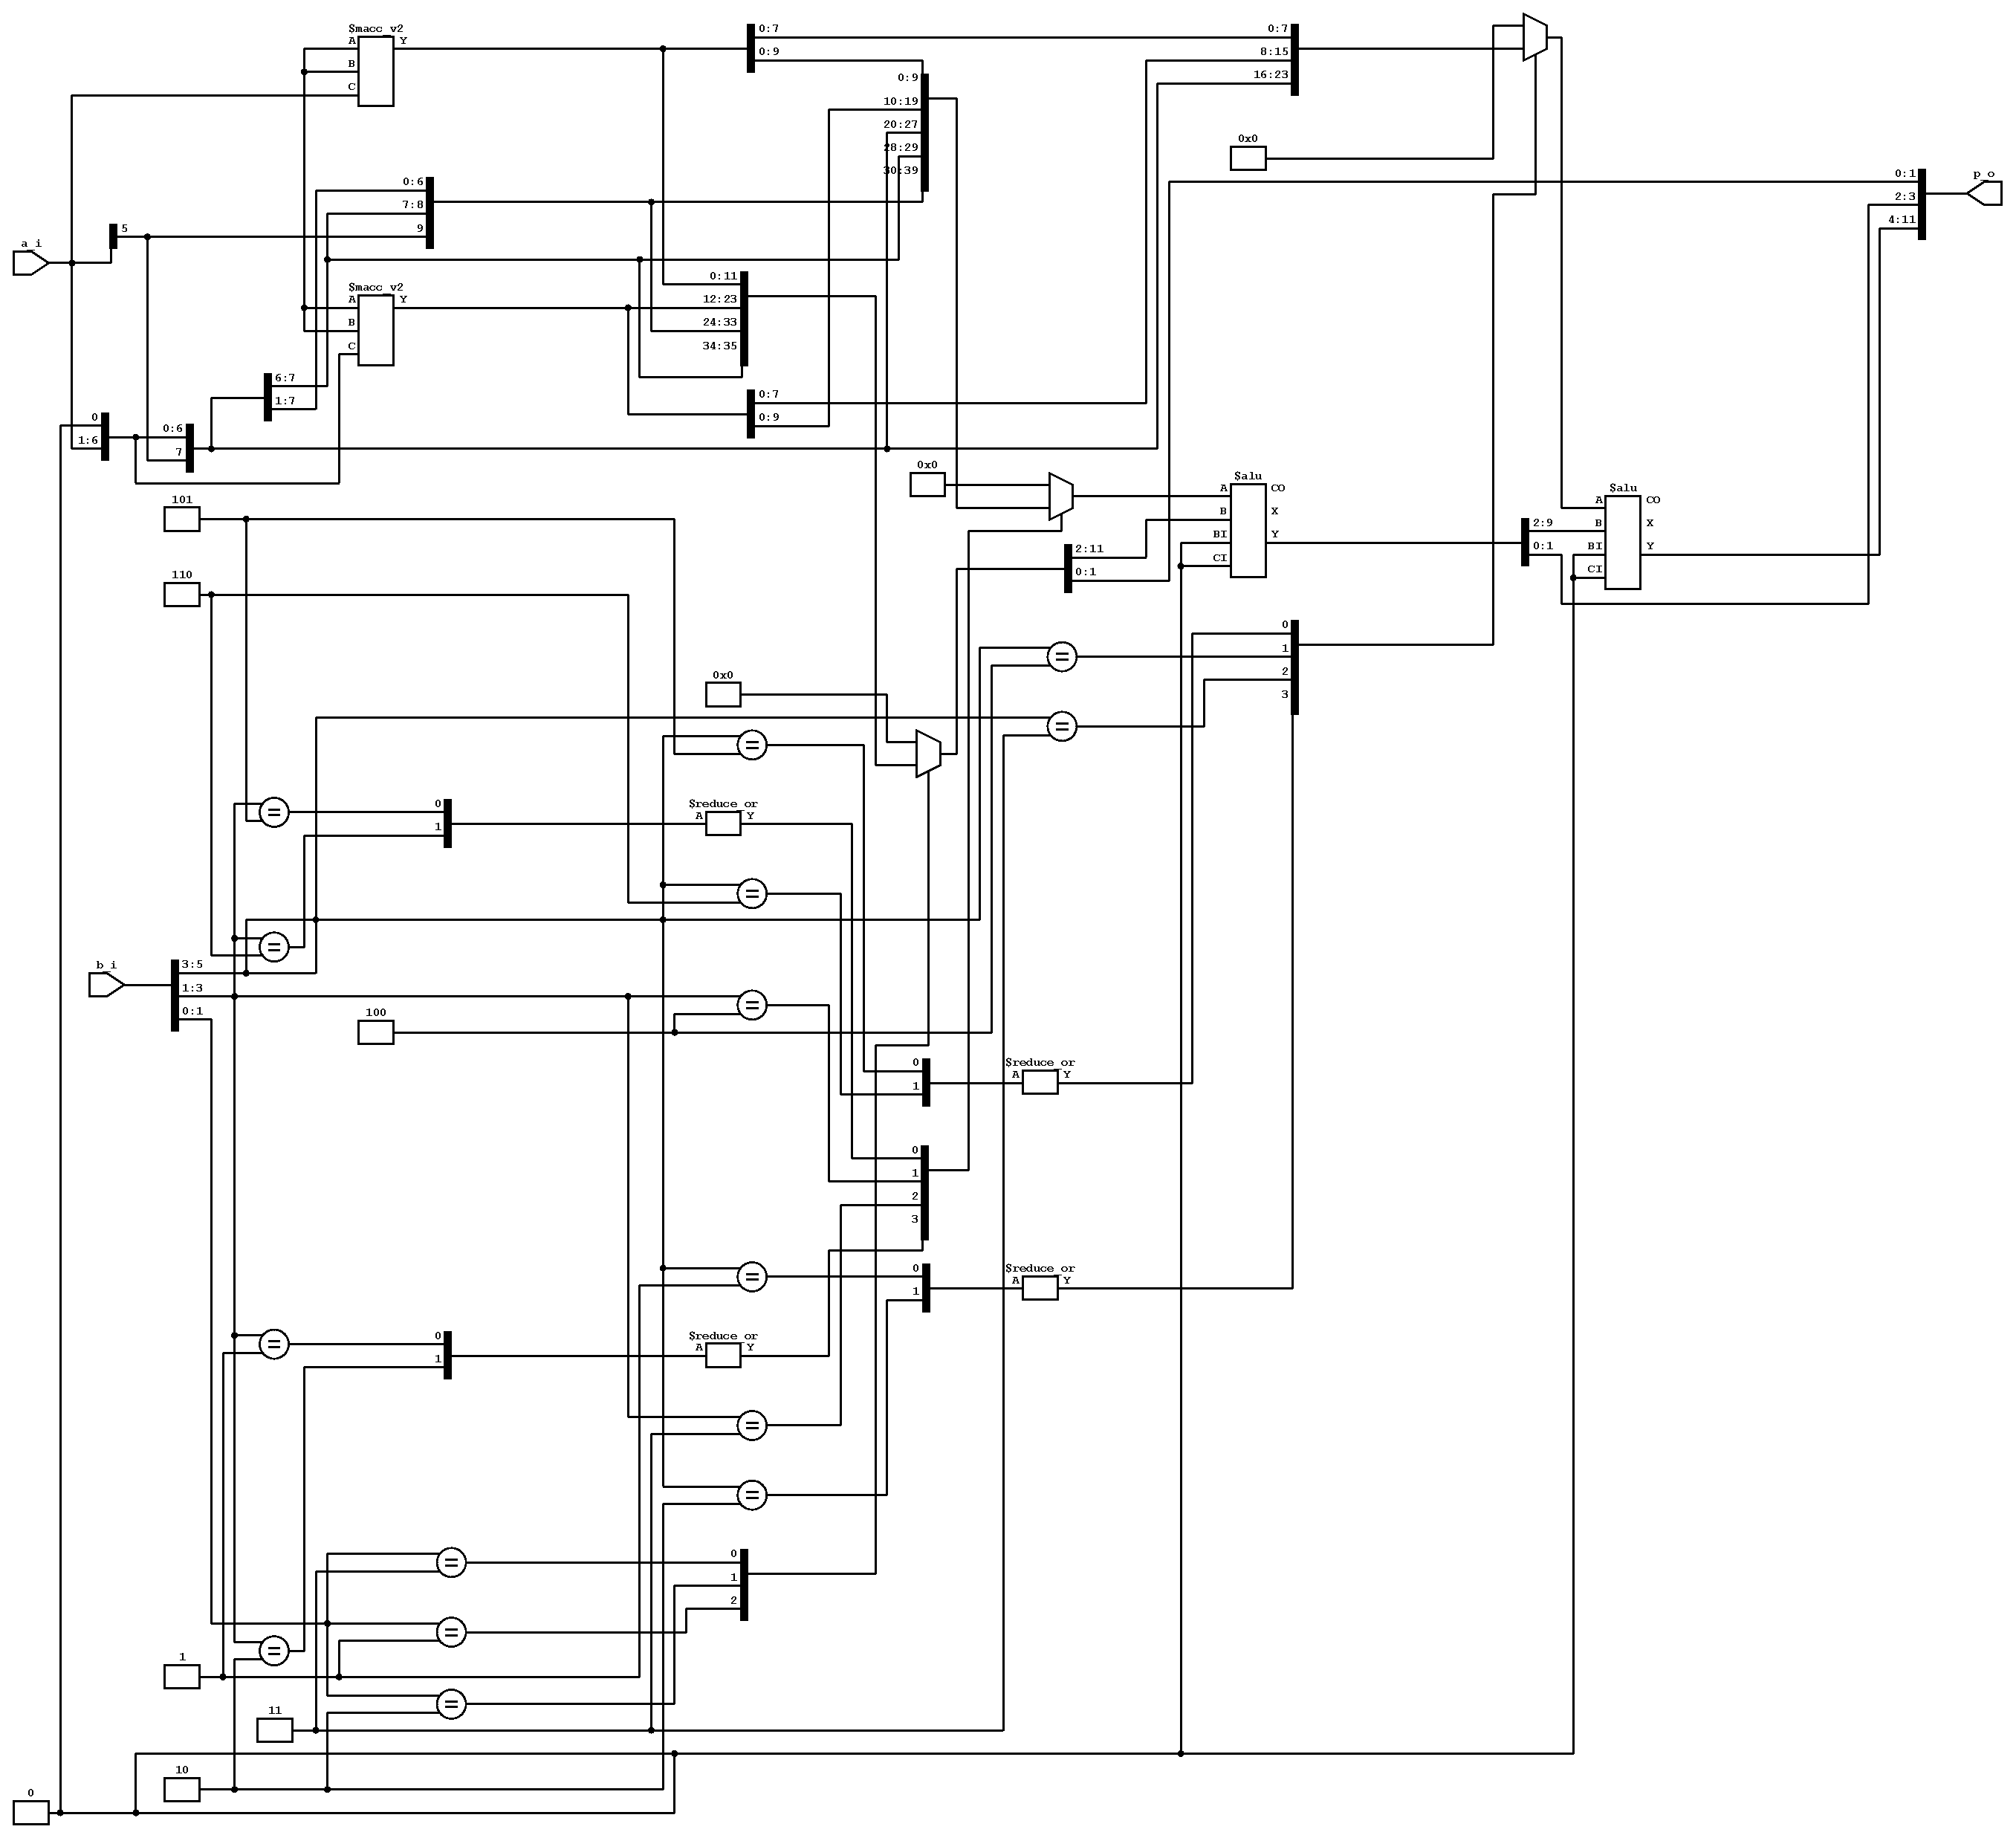
\includegraphics[width=0.92\linewidth]{figures/sch_booth_w6.pdf}
  \caption{Yosys RTL schematic of \code{booth\_multiplier} with $W=6$
    (word-level cells: \code{\$eq} group decoders, Booth-recoding \code{\$pmux}, partial-product \code{\$macc}/\code{\$alu}).}
  \label{fig:sch_booth}
\end{figure}

\begin{figure}[H]
  \centering
  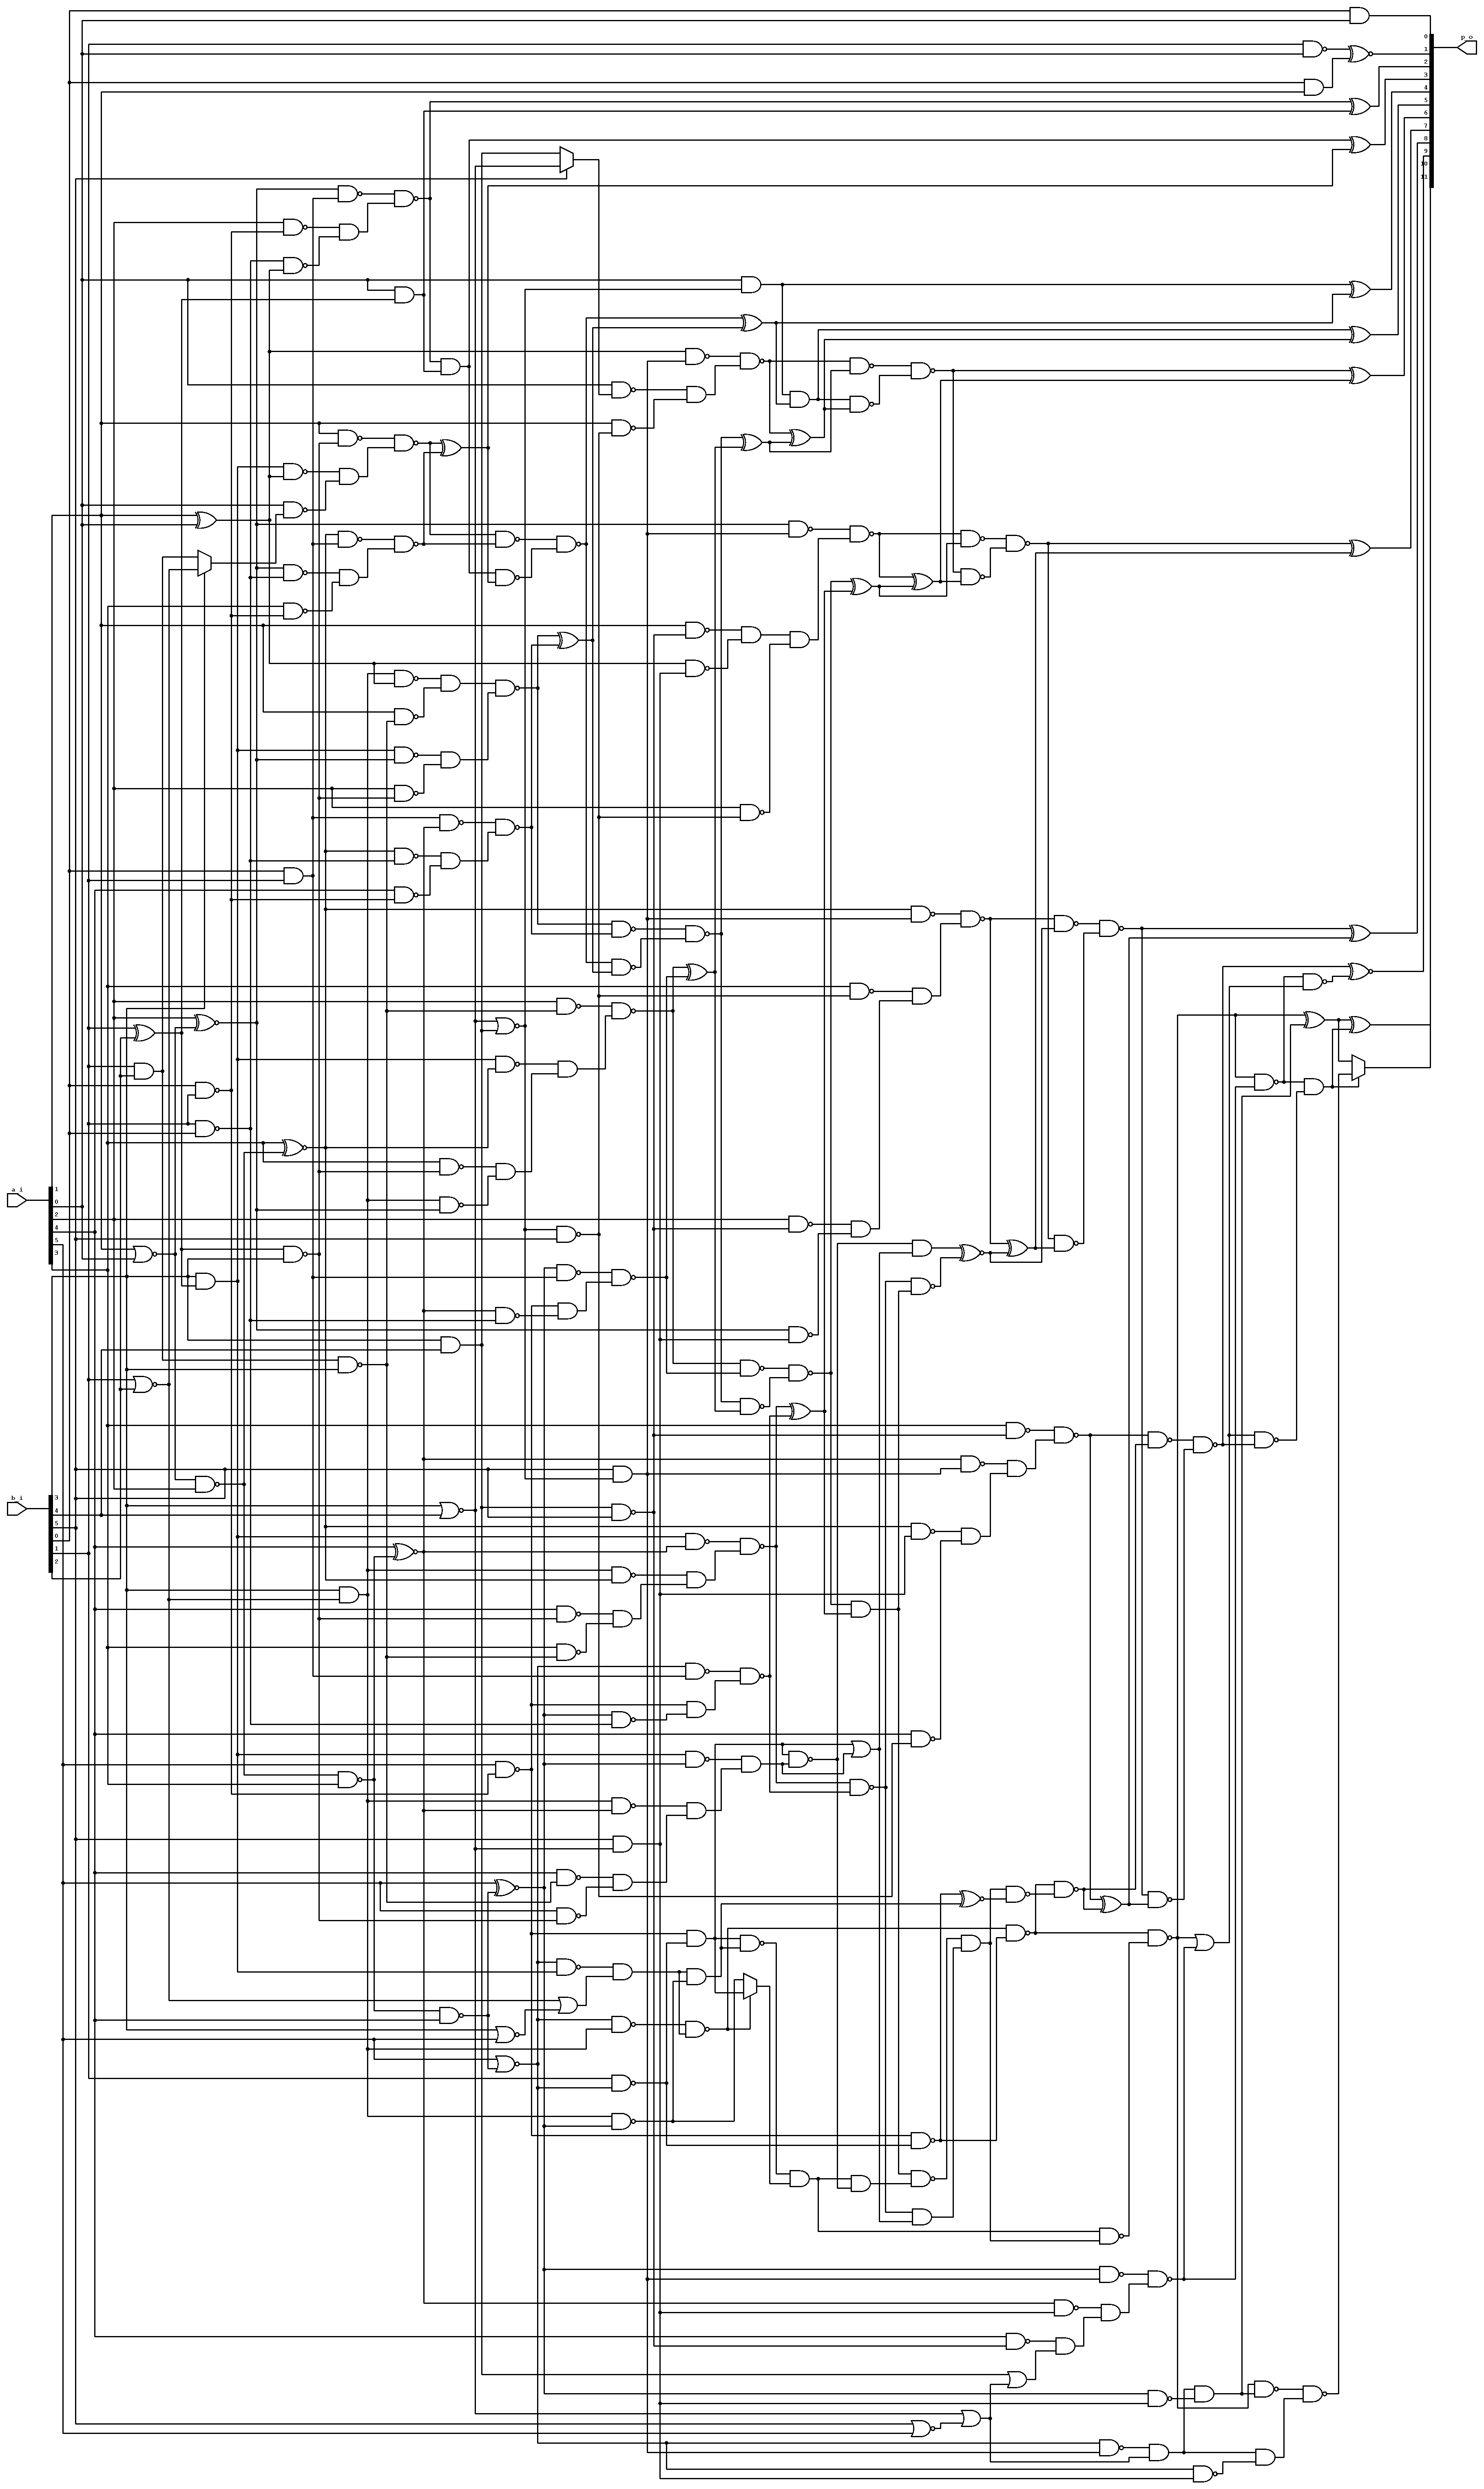
\includegraphics[height=0.80\textheight]{figures/sch_booth_w6_gates.pdf}
  \caption{The same 6-bit Booth multiplier after gate-level synthesis (216 gates).}
  \label{fig:sch_booth_g}
\end{figure}

\begin{figure}[p]
  \centering
  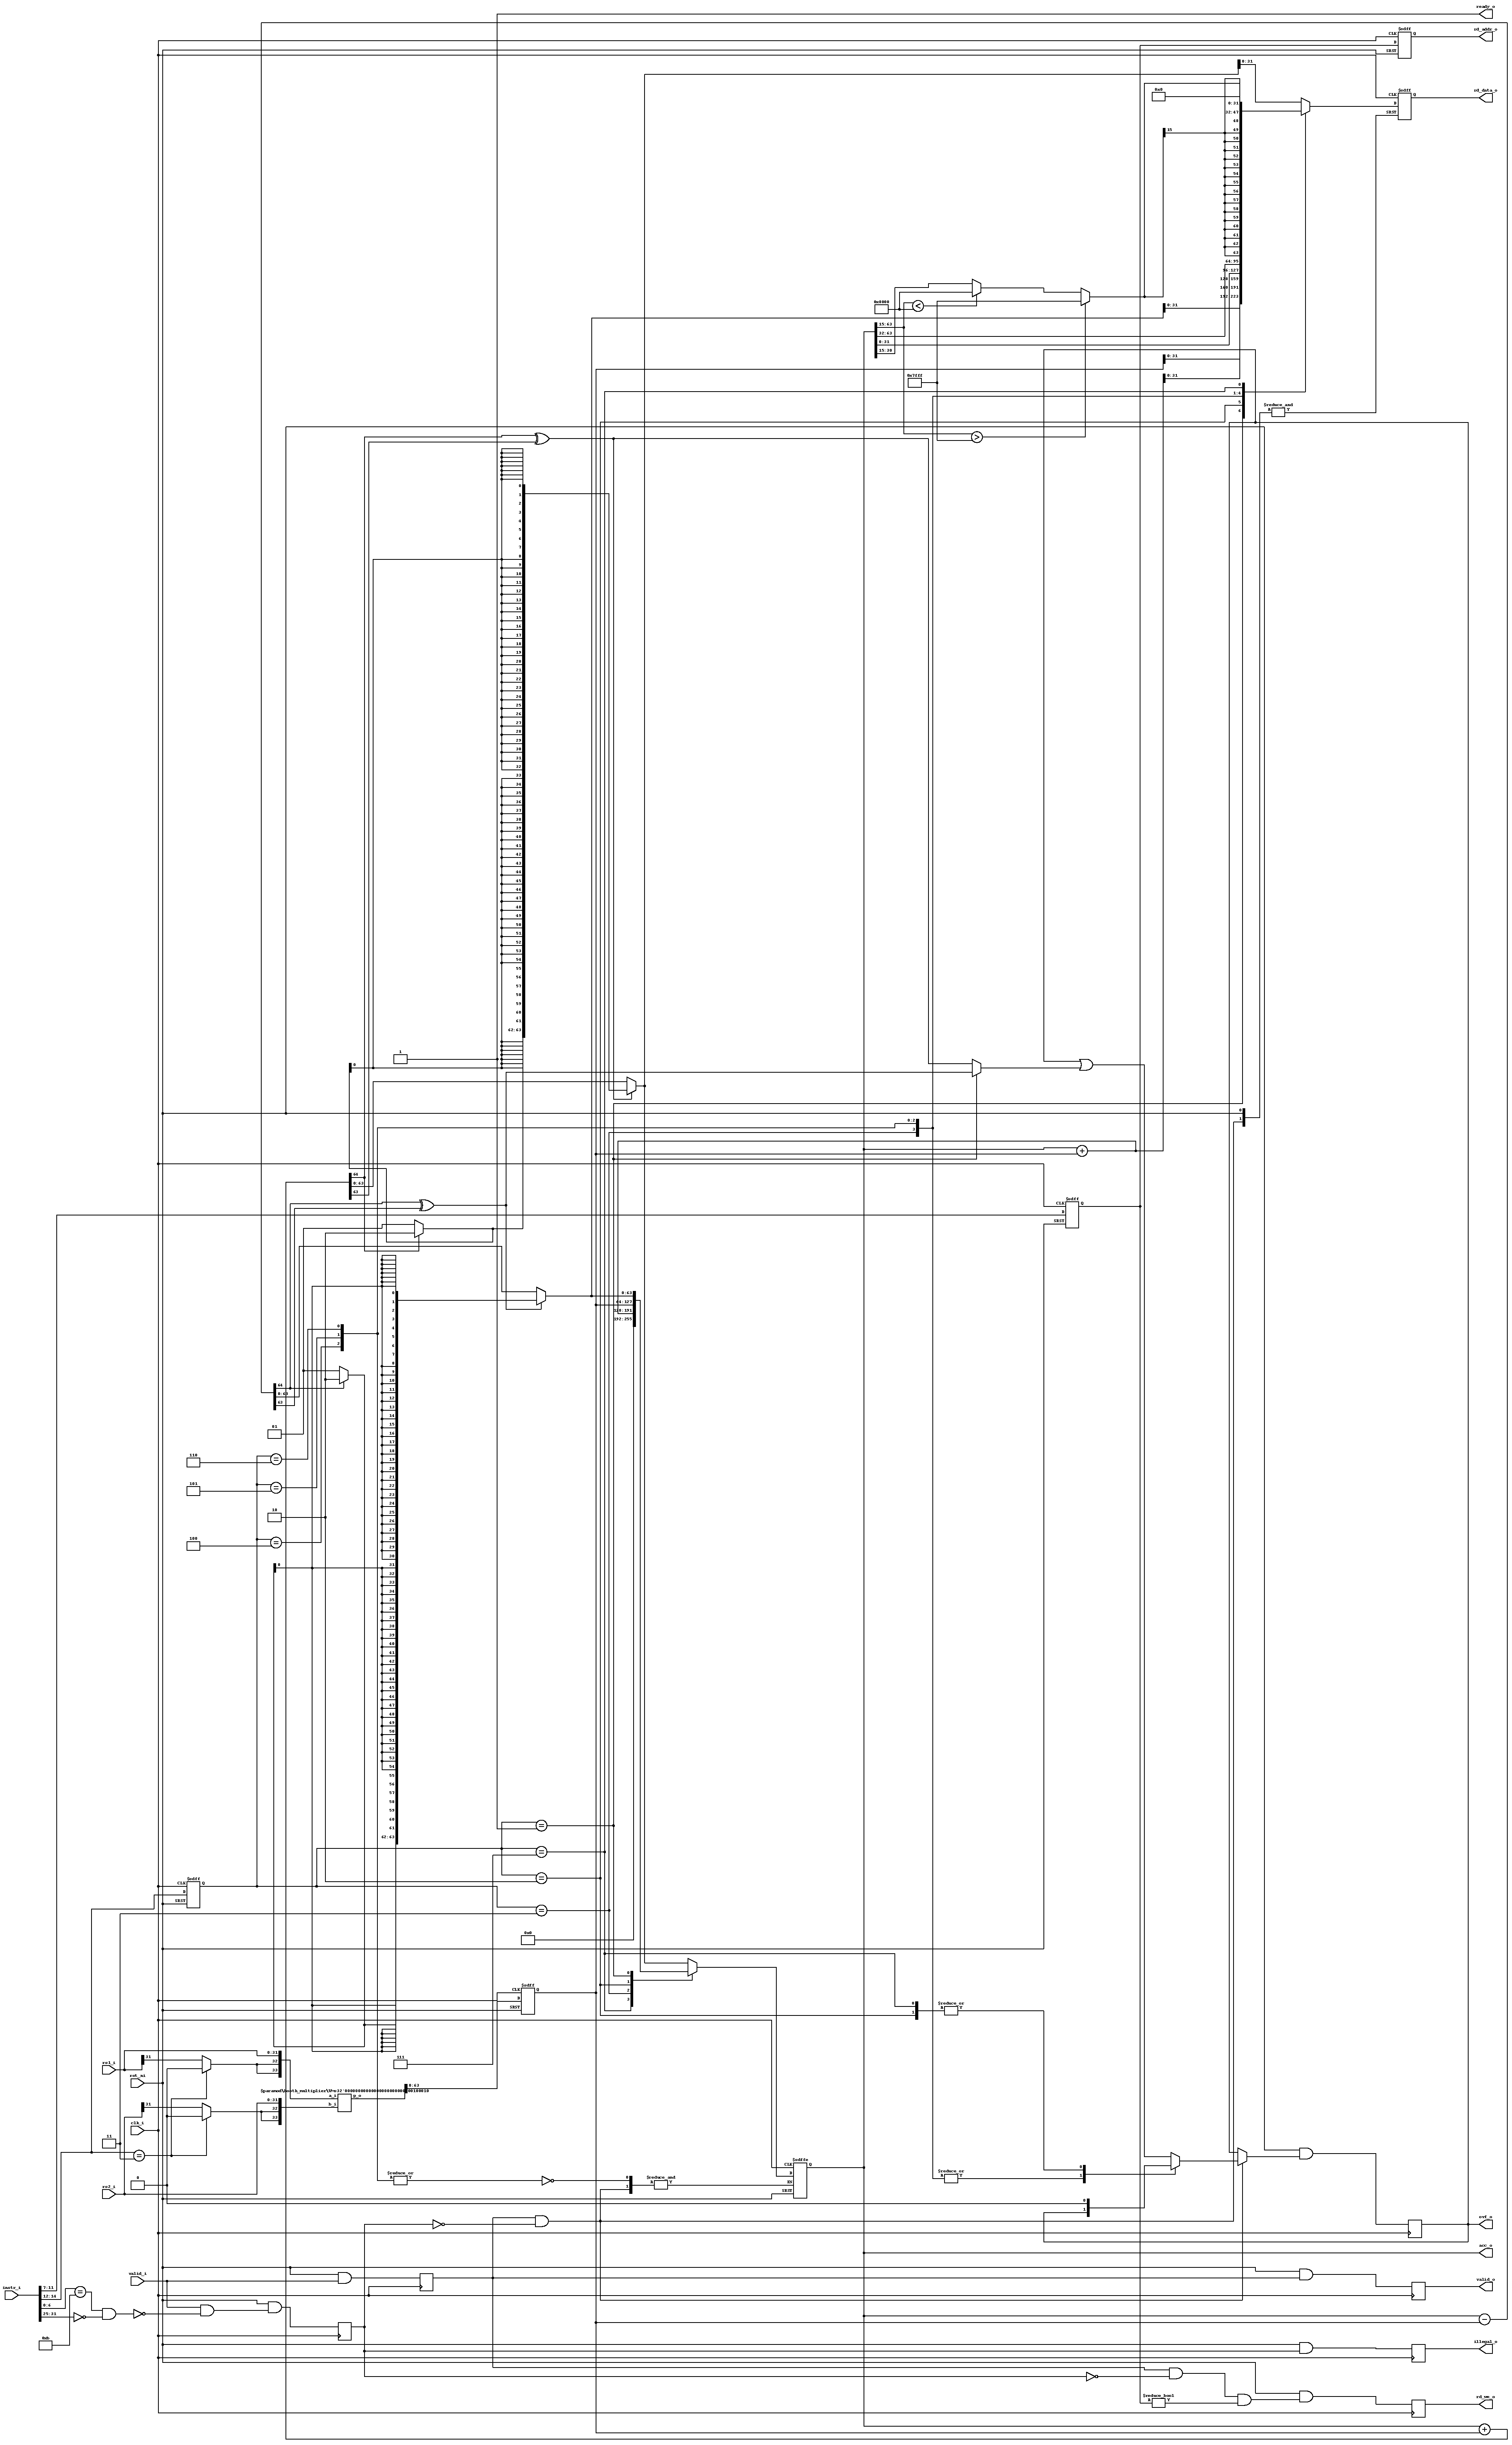
\includegraphics[height=0.86\textheight]{figures/sch_mac_unit.pdf}
  \caption{Yosys RTL schematic of the complete \code{mac\_unit} (Booth
    multiplier shown as a single block).}
  \label{fig:sch_mac}
\end{figure}

\section{Generic gate-level synthesis of the MAC unit}
The flow \code{synth -flatten} followed by
\code{abc -g AND,NAND,OR,NOR,XOR,XNOR,ANDNOT,ORNOT,MUX} produces the netlist
summarised in Table~\ref{tab:gen} and Figure~\ref{fig:syncells}.
\code{check -assert} reports no combinational loops, no multiple drivers,
no undriven nets and no inferred latches.

\begin{table}[H]
  \centering
  \caption{Generic synthesis result (flattened \code{mac\_unit}).}
  \label{tab:gen}
  \small
  \begin{tabular}{@{}lr@{\qquad}lr@{}}
    \toprule
    Cell type & Count & Cell type & Count \\
    \midrule
    NAND   & 5027 & NOT    & 74 \\
    AND    & 1785 & MUX    & 32 \\
    XOR    & 1459 & DFF, sync.\ reset (\code{\$\_SDFF\_})         & 114 \\
    OR     & 376  & DFF, sync.\ reset + enable (\code{\$\_SDFFE\_}) & 65 \\
    NOR    & 226  & \textbf{Total cells} & \textbf{9532} \\
    XNOR   & 199  & \textbf{Flip-flops} & \textbf{179} \\
    ANDNOT / ORNOT & 96 / 79 & Est.\ transistors (\code{stat -tech cmos}) & $\approx$55{,}456 \\
    \bottomrule
  \end{tabular}
\end{table}

\begin{figure}[H]
  \centering
  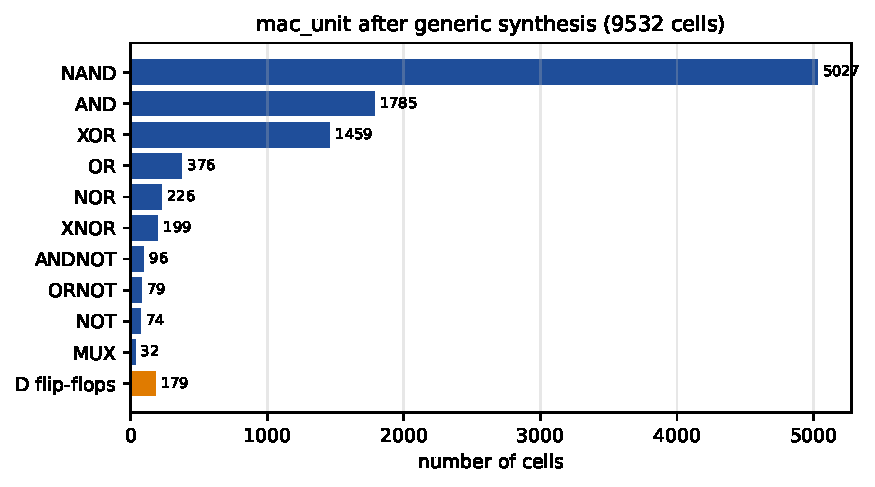
\includegraphics[width=0.75\linewidth]{figures/syn_cells.pdf}
  \caption{Cell-type distribution of the synthesised MAC unit.}
  \label{fig:syncells}
\end{figure}

\paragraph{Register count check.}
The 179 flip-flops match the RTL exactly. Stage~1 holds $1+1+3+5+64=74$ bits
(valid, illegal, \code{funct3}, \code{rd}, product), while stage~2 holds
$64+1+1+5+1+32+1=105$ bits (ACC, OVF, valid, \code{rd}, write enable, data,
illegal). The 65 flip-flops with an enable input are the accumulator and the
OVF flag.
They keep their value on read-only instructions; Yosys inferred the enable
from the default assignment \code{acc\_nxt = acc\_q}.

\paragraph{Logic depth.}
The longest combinational path (\code{ltp}) is \textbf{127 gate levels}, from
the operands through the multiplier to \code{s1\_prod[63]}. For comparison,
the Booth module was replaced by \code{*} and synthesised with Yosys' own
Booth-encoder + Wallace-tree generator (\code{synth -booth}). That version uses
21\,\% fewer gates (7{,}541) but its depth is the same (128 levels). In both
cases, the depth comes from the ripple-carry carry-propagate adders, which
account for about two gate levels per bit, not from the partial-product
reduction.

\section{Area breakdown: MAC unit and complete processor}
Figure~\ref{fig:synarea} compares the hierarchical gate counts. In the
stand-alone MAC unit, the Booth multiplier accounts for 79\,\% of the logic
(7{,}852 of 9{,}990 cells). The complete processor, synthesised by the
script \code{synth/synth\_core.ys}, contains 25{,}286 gates in total. Of these, the
RV32 pipeline makes up 15{,}303, which includes the register file implemented
as 1{,}024 flip-flops (the generic flow has no RAM cells) together with the
RV32M 33$\times$33 multiplier; the MAC unit's control and accumulator take
2{,}138 gates; and the Booth multiplier takes 7{,}845 gates. Adding the full
DSP extension therefore costs about 40\,\% of the processor's gate count.

\begin{figure}[H]
  \centering
  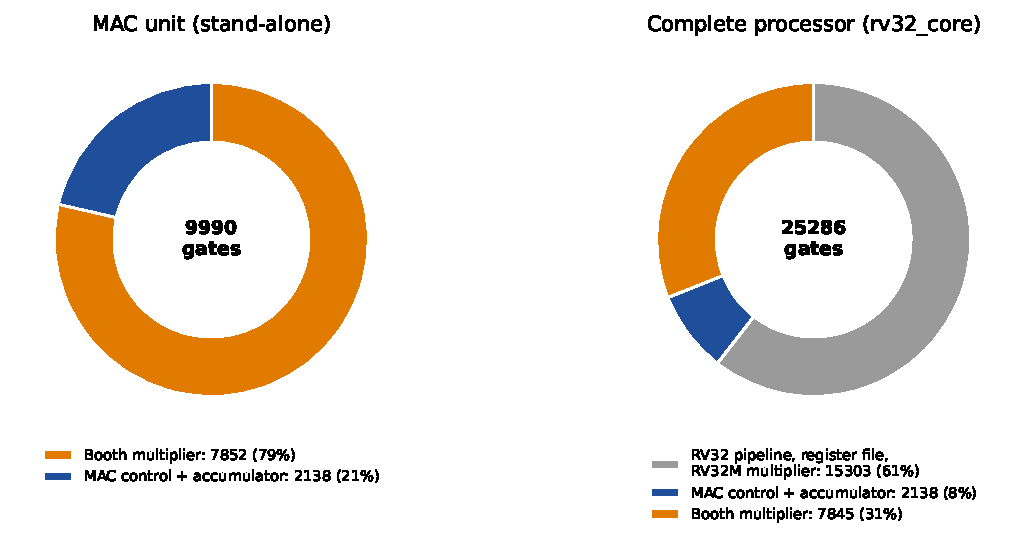
\includegraphics[width=\linewidth]{figures/syn_area.pdf}
  \caption{Generic-gate area breakdown of the MAC unit and of the complete processor.}
  \label{fig:synarea}
\end{figure}

\section{FPGA implementation on the Lattice ECP5}
Three designs were placed and routed. Design~A is the MAC unit with the Booth
multiplier, in which the radix-4 Booth multiplier is built from LUTs and carry
chains. Design~B is the MAC unit with DSP multipliers: the Booth module is
replaced by \code{synth/native\_multiplier.v} (\code{*}), so the
multiplication maps onto four hard \code{MULT18X18D} blocks, and it serves as
a comparison point only. Design~C is the complete processor, \code{rv32\_core}
including the MAC unit with the Booth multiplier; here the register file maps
to 32 LUT-RAM blocks and the RV32M multiplier to DSP blocks, while the
instruction and data memories are outside the core.
For A and B, the unit is wrapped in \code{synth/fmax\_wrapper.v}, which
registers every input and output, so that every timing path is
register-to-register, as it would be inside a processor.

\begin{table}[H]
  \centering
  \caption{ECP5 LFE5U-85F implementation results (post place \& route).}
  \label{tab:ecp5}
  \small
  \begin{tabular}{@{}lrrr@{}}
    \toprule
    Metric & A: MAC (Booth) & B: MAC (DSP) & C: RV32IM core + MAC \\
    \midrule
    LUT4 (Yosys)                     & 5{,}108 & 611 & 6{,}486 \\
    PFUMX / L6MUX21 (wide muxes)     & 1{,}855 / 584 & 210 / 52 & 1{,}992 / 631 \\
    CCU2C (carry cells)              & 155 & 162 & 399 \\
    Flip-flops (design)              & 179 & 179 & 730 \\
    LUT-RAM blocks (DPR16X4)         & 0 & 0 & 32 \\
    MULT18X18D (DSP multipliers)     & 0 & 4 & 4 \\
    Logic cells after P\&R           & 4{,}854 (5.8\,\%) & 963 (1.2\,\%) & 7{,}566 (9.0\,\%) \\
    I/O pins                         & 204 & 204 & 330 \\
    \midrule
    Critical path (reg $\rightarrow$ reg) & 17.73\,ns & 12.69\,ns & 28.94\,ns \\
    \quad of which logic / routing   & 6.0 / 11.8\,ns & 7.9 / 4.8\,ns & 10.1 / 18.9\,ns \\
    \textbf{Maximum frequency $F_{\max}$} & \textbf{56.4\,MHz} & \textbf{78.8\,MHz} & \textbf{34.6\,MHz} \\
    \bottomrule
  \end{tabular}
\end{table}

\begin{figure}[H]
  \centering
  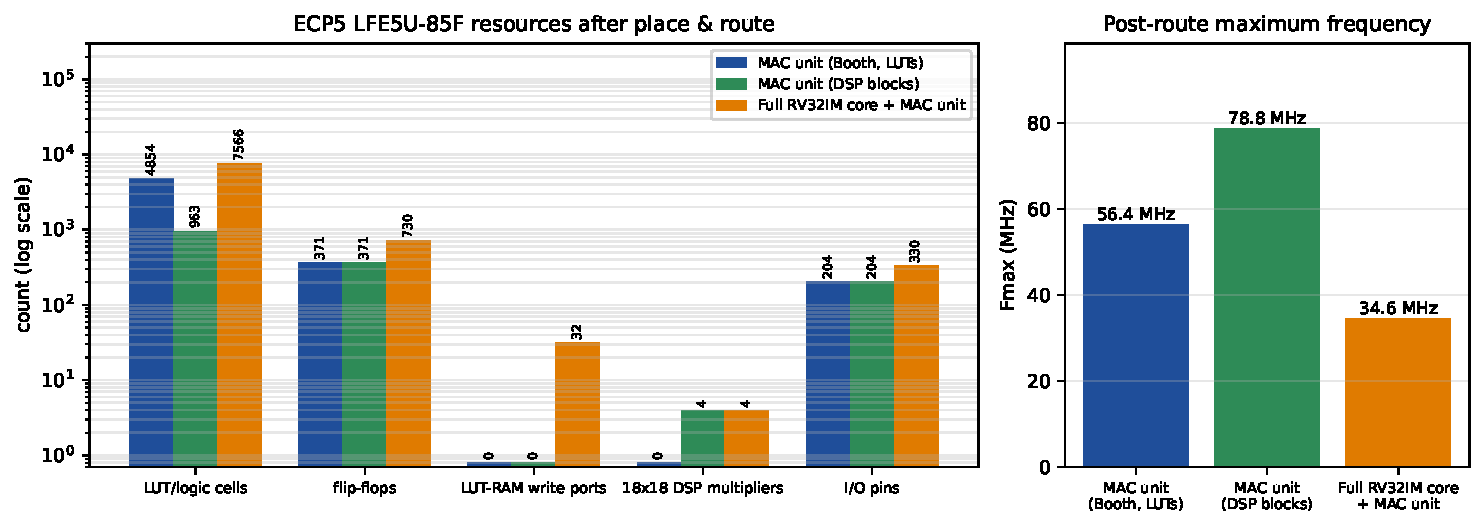
\includegraphics[width=\linewidth]{figures/fpga_resources.pdf}
  \caption{ECP5 resource usage (log scale) and post-route $F_{\max}$ of the three designs.}
  \label{fig:fpgares}
\end{figure}

\paragraph{Critical paths.}
Figure~\ref{fig:critpath} plots the cumulative delay along each design's
critical path, as reported by nextpnr. For designs A and B, the path starts at
the input operand register, passes through the stage-1 multiplier and ends at
the \code{s1\_prod} pipeline register; the stage-2 accumulate path is shorter,
which confirms that the MAC pipeline is split in the right place. In the Booth
version, routing (11.8\,ns) dominates logic (6.0\,ns), because the LUT-based
multiplier is spread over a large area. For the complete processor, the
critical path runs from the WB forwarding control, through the forwarding
multiplexer and the \emph{single-cycle RV32M multiplier} (DSP blocks plus
carry-chain adders), to the EX/MEM result register, so in the full CPU it is
the baseline \code{mul} instruction, not the pipelined MAC unit, that limits
the clock.

\begin{figure}[H]
  \centering
  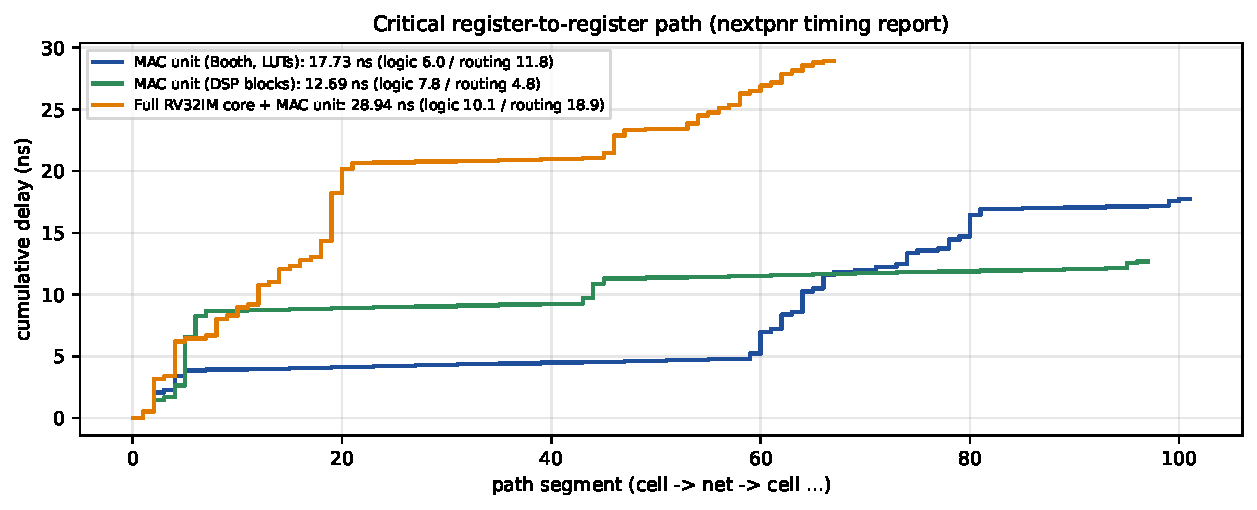
\includegraphics[width=\linewidth]{figures/fpga_critpath.pdf}
  \caption{Cumulative delay along the critical register-to-register path of each design.}
  \label{fig:critpath}
\end{figure}

\begin{figure}[H]
  \centering
  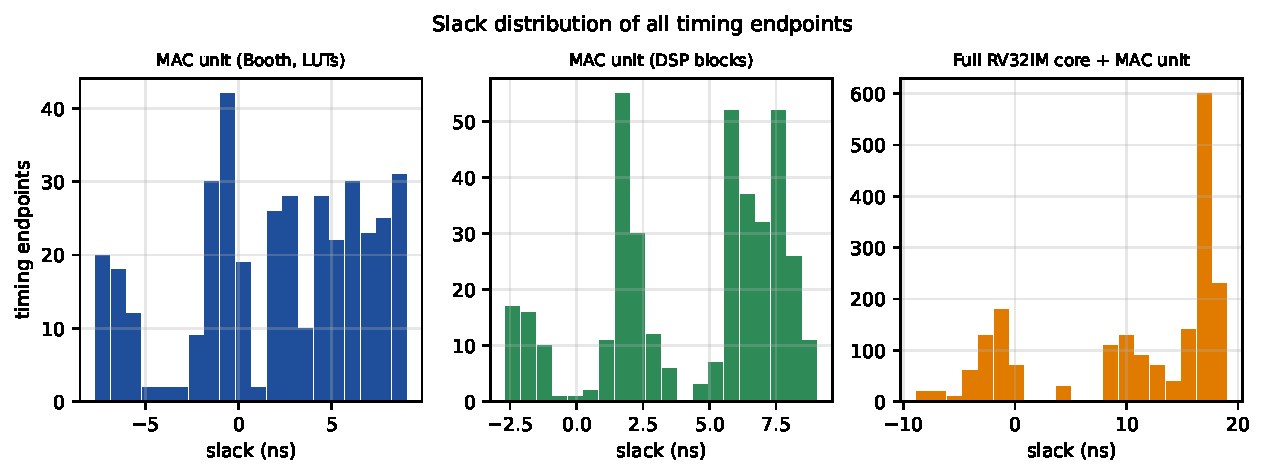
\includegraphics[width=\linewidth]{figures/fpga_slack.pdf}
  \caption{Slack histograms of all timing endpoints (100\,MHz target for A/B, 50\,MHz for C).}
  \label{fig:slack}
\end{figure}

\paragraph{Floorplans.}
Figures~\ref{fig:fp_mac} and~\ref{fig:fp_core} are die renders of the
placed-and-routed designs, drawn from nextpnr's output
(\code{report/scripts/export\_floorplan.py}). Each square is one programmable
tile of the ECP5 die (tile coordinates X\,0--126, Y\,0--95), coloured by the
block whose cells nextpnr placed there; brighter means more cells in the tile.
The copper glow underneath is the routing density (routed wire segments per
tile, log scale), the ring of small squares is the used I/O pads, and the
white line is the critical path, from its start (dot) to its end (star). An
interactive version, with zoom, per-block highlighting and a per-tile
breakdown, is on the project page. The Booth multiplier (orange) forms one
dense block, with the MAC stage-2 logic (blue) at its edge, and it is the
routing hot spot. In the complete processor, the core logic, the MAC unit and
the four DSP blocks are packed into one region in the upper-left corner, close
to the I/O pins on the top edge.

\begin{figure}[H]
  \centering
  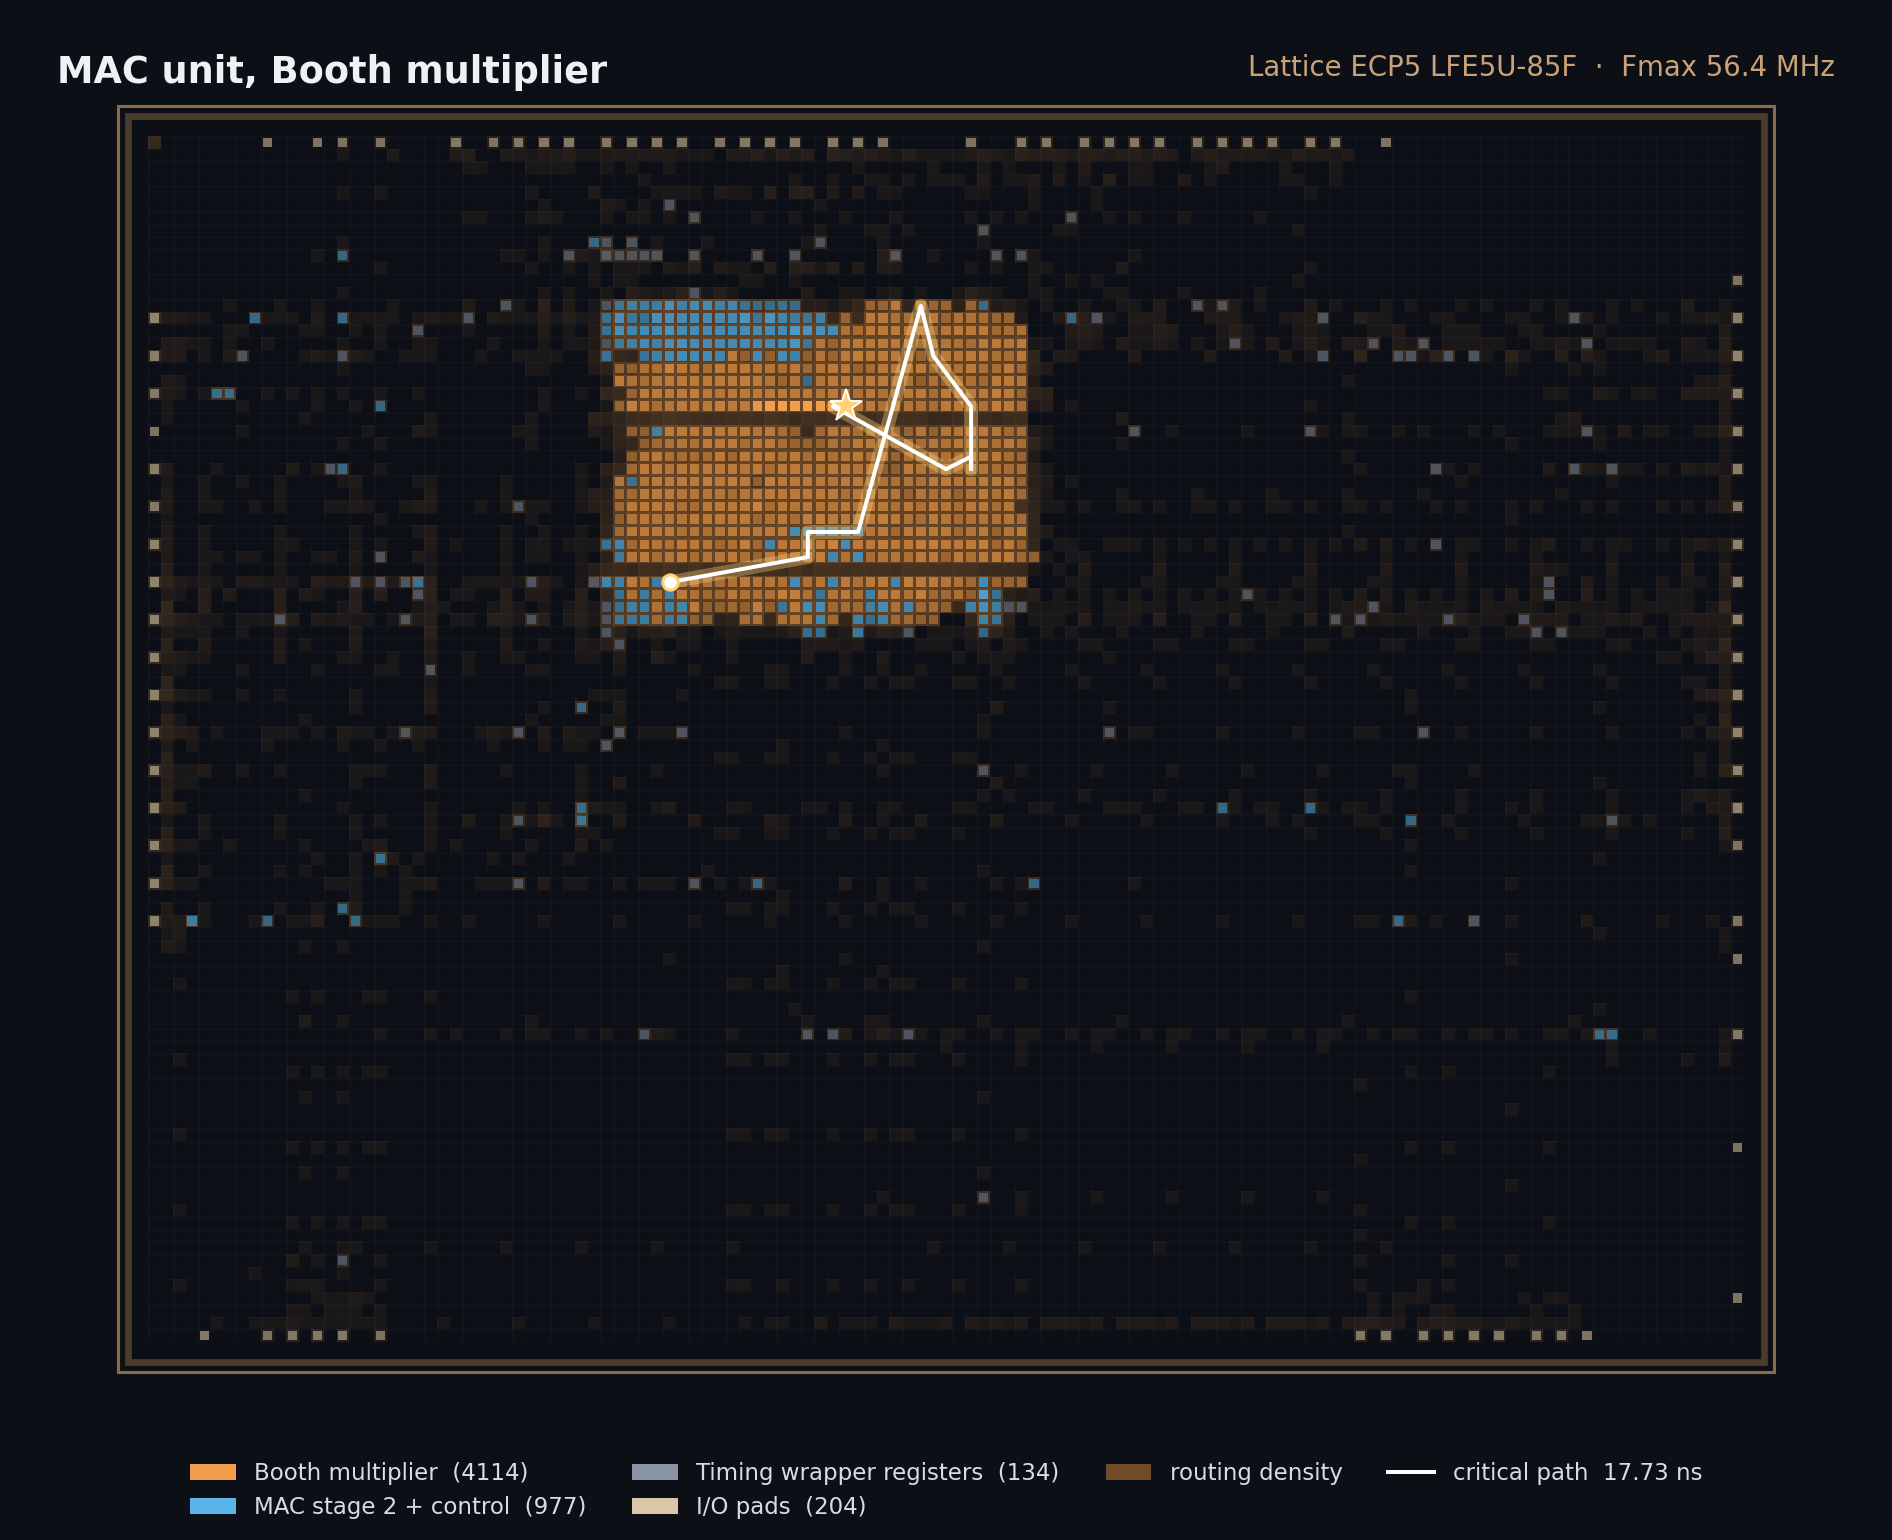
\includegraphics[width=0.92\linewidth]{figures/floorplan_mac.png}
  \caption{Die render of the MAC unit (design A) on the ECP5: placement by
    block, routing density and critical path.}
  \label{fig:fp_mac}
\end{figure}

\begin{figure}[H]
  \centering
  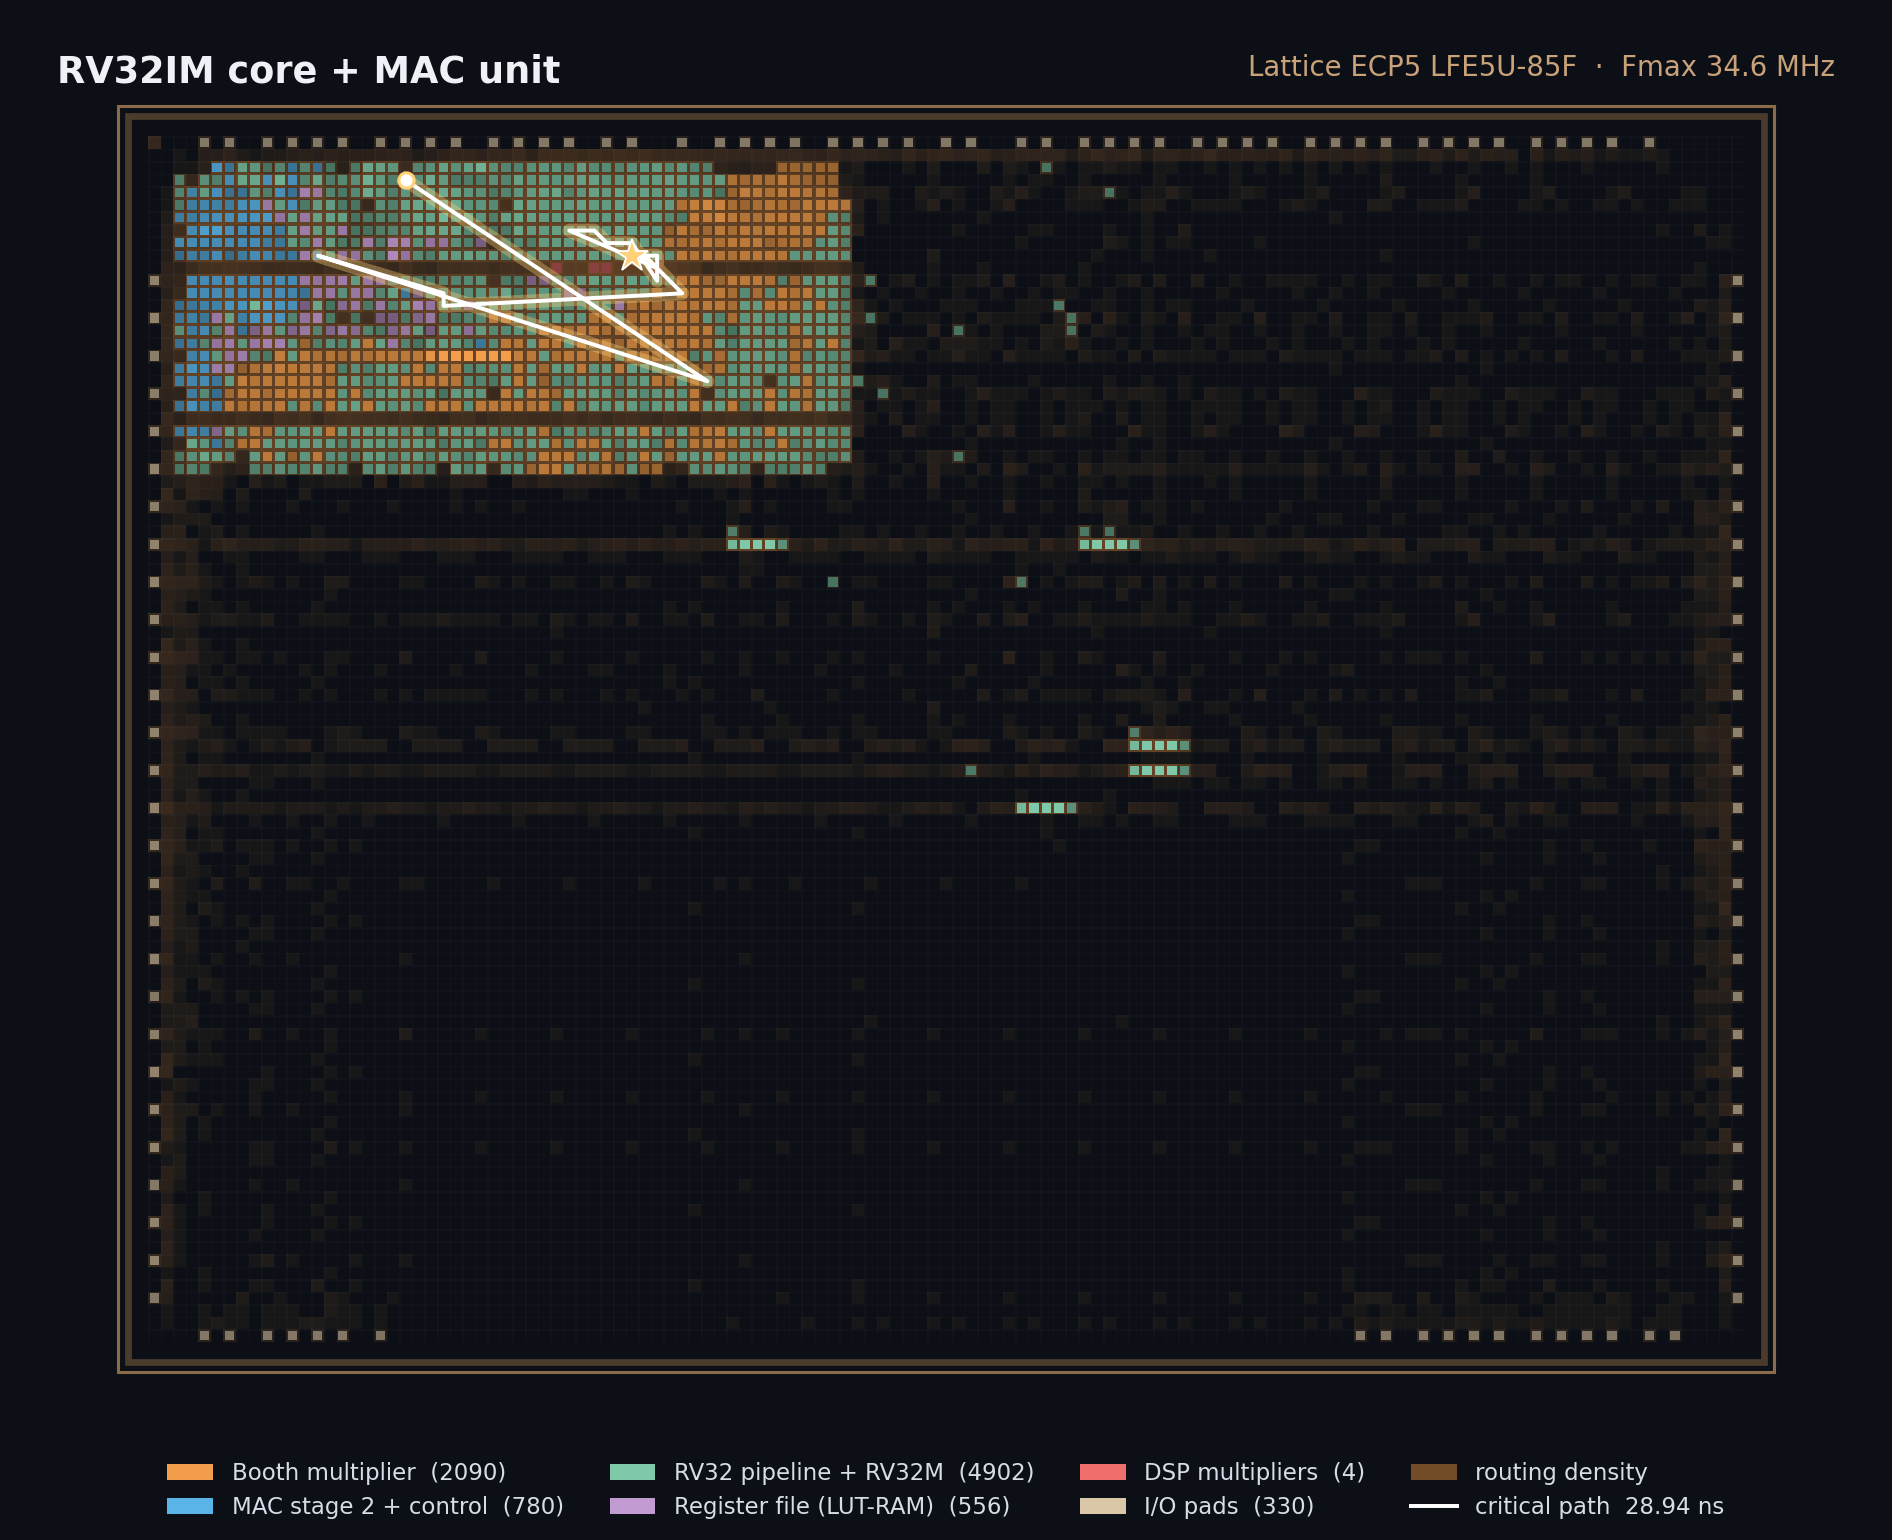
\includegraphics[width=0.92\linewidth]{figures/floorplan_core.png}
  \caption{Die render of the complete RV32IM core with the MAC unit (design C).
    The register file (purple) sits next to the MAC unit; the critical path
    runs through the RV32M multiplier on the DSP blocks.}
  \label{fig:fp_core}
\end{figure}

\paragraph{Interpretation.}
On an FPGA, the hand-written Booth multiplier uses about 8$\times$ more LUTs
than the DSP version and is 28\,\% slower. This is expected, because FPGAs
contain hard multipliers. The Booth design is still the right choice for this
project: it shows the algorithm explicitly, it is fully portable, and it is
what an ASIC implementation would use. For an FPGA product, variant~B would
be preferred.

\section{Post-synthesis gate-level simulation}
The flattened gate-level netlist written by Yosys
(\code{synth/out/mac\_unit\_netlist.v}, about 19{,}000 lines) was simulated with
the \emph{unchanged} testbench \code{tb\_mac\_unit.v}. It passed all tests
(Listing~\ref{lst:gate}). This confirms that synthesis preserved the
behaviour of the RTL and that there are no simulation/synthesis mismatches.
The gate-level simulation has zero delay, so it checks function only; timing
is covered by the static timing analysis above.

\begin{lstlisting}[style=log, caption={Gate-level simulation result (\code{sim/gate/mac\_gate\_sim.log}).}, label={lst:gate}]
 FUNCTIONAL COVERAGE
   mac=570 msu=338 mul.acc=378 macu=381 rdacc.lo=346 rdacc.hi=386 rdacc.q15=393 clracc=374
   illegal=162  saturation events=7  rd=x0 writes=360  bubble gaps=684
 RESULTS
   instructions issued : 3328
   checks performed    : 3351
   errors              : 0
   >>> ALL TESTS PASSED <<<
\end{lstlisting}

%===========================================================================
\chapter{Discussion}\label{ch:disc}
%===========================================================================

\section{Design trade-offs}
\textbf{Dedicated accumulator vs.\ register-file accumulation.} A
dedicated 64-bit accumulator gives full precision and needs only two
register-file read ports. The cost is extra architectural state, which
an operating system must save on a context switch, and explicit
\code{rdacc} instructions to read the result. The Xpulp
\code{p.mac}~\cite{cv32e40p} approach needs a third read port and
accumulates in only 32 bits.

\textbf{Saturation vs.\ wrap-around.} Signed operations saturate,
which is the expected DSP behaviour, whereas \code{macu} wraps modulo $2^{64}$,
which is what checksums and hashing need.

\textbf{Two-stage MAC pipeline aligned with the CPU pipeline.} Putting
the multiplication in EX and the accumulation in MEM means MAC
instructions issue back-to-back with no forwarding inside the unit.
Only a consumer placed \emph{directly} after a MAC result pays one
stall cycle, exactly like a load, and in the scheduled FIR code this never
happens.

\textbf{Instruction count vs.\ loop overhead.} The MAC instructions
cut the arithmetic work per tap from six instructions to one. In the
looped FIR, however, loads and loop control remain, so the measured
speed-up is 1.59$\times$. Once the loop overhead is removed by
unrolling, the MAC unit's advantage grows to 2.67$\times$. Adding
post-increment loads or hardware loops (as in Xpulp) would bring the
looped code close to the unrolled performance.

\section{Limitations}
The synthesis results come from open-source tools and a generic gate library.
No commercial ASIC standard-cell library was used, so the report gives gate
counts and logic depth rather than area in $\mu$m$^2$ or power figures. The MAC
unit's critical path is the 34$\times$34-bit combinational Booth multiplier
(17.7\,ns on ECP5, 127 gate levels), whose partial products are summed with
ripple-carry adders. The processor implements the RV32M multiply instructions
in a single cycle, which is simple but sets the processor's critical path
(28.9\,ns, 34.6\,MHz on ECP5). It has no caches, interrupts, CSRs or division
instructions, and its memories are modelled with combinational reads; on an
FPGA they would be replaced by synchronous block RAM, which requires an extra
fetch stage or registered addresses. Finally, the programs are written in
assembly with a project-specific assembler, and C code would need compiler
support for the custom instructions, for example through inline assembly.

\section{Future work}
Several extensions would build on this work. The critical paths could be
shortened by using a carry-save (Wallace/Dadda) tree with a parallel-prefix
final adder (for example Kogge-Stone) for the Booth multiplier, and by
pipelining the RV32M multiplier over EX and MEM, as is already done for the MAC
unit. Post-increment loads and a zero-overhead hardware loop could be added so
that looped DSP code reaches the throughput of the unrolled code, and
packed-SIMD operations (for example two 16$\times$16 MACs per cycle), similar
to the RISC-V P-extension proposals, would widen the arithmetic. The
instruction and data memories could be mapped to FPGA block RAM so that the
processor runs on a real ECP5 board, and the design could be taken through an
ASIC flow with a real standard-cell library (for example OpenLane with the
SkyWater 130\,nm PDK). Finally, the Booth multiplier could be formally verified
against \code{*}, for example with SymbiYosys.

%===========================================================================
\chapter{Conclusion}\label{ch:concl}
%===========================================================================
This project designed a RISC-V custom-extension multiply-accumulate unit for
digital signal processing, integrated it into a complete 5-stage pipelined
RISC-V processor, and verified both thoroughly. The MAC unit adds eight
\code{custom-0} instructions and is built around a radix-4 Booth multiplier
and a 64-bit saturating accumulator with Q15 support. Its two-stage pipeline
accepts one instruction per cycle and lines up exactly with the EX and MEM
stages of the processor.

At the unit level, an independent reference model and scoreboard, exhaustive
multiplier tests, directed corner cases, three analytical DSP benchmarks and a
3{,}000-instruction constrained-random regression performed 88{,}896 checks,
all with zero errors.

At the system level, real RISC-V programs, built with a project-specific
assembler, ran on the processor: an 18-part ISA and hazard self-test, and a
16-tap low-pass FIR over 128 samples in four versions. Every program passed.
The FIR outputs were bit-identical to the golden model, the unwanted tone was
attenuated by 60.1\,dB as the filter design predicts, and mutation tests
confirmed that the system tests detect forwarding and stall bugs. Compared with
the same filter in plain RV32IM software, the MAC instructions made the FIR
1.59$\times$ faster in looped form and 2.67$\times$ faster in unrolled form,
with 2.6$\times$ smaller code.

Yosys synthesis produced a latch-free MAC netlist of 9{,}532 gates and 179
flip-flops, which passes the full testbench at gate level. On a Lattice ECP5
FPGA, the MAC unit reaches 56.4\,MHz, and the complete processor with the
MAC unit reaches 34.6\,MHz using 9\,\% of the device's logic. The schematics,
floorplans and timing analysis show that the multipliers, both the Booth
multiplier and the RV32M multiplier, are the largest blocks and set the
critical paths. That makes them the main target for future optimisation.


%===========================================================================
% References
%===========================================================================
\begin{thebibliography}{99}
\addcontentsline{toc}{chapter}{References}

\bibitem{booth}
A.~D. Booth, ``A signed binary multiplication technique,''
\emph{Quarterly Journal of Mechanics and Applied Mathematics}, vol.~4, no.~2,
pp.~236--240, 1951.

\bibitem{macsorley}
O.~L. MacSorley, ``High-speed arithmetic in binary computers,''
\emph{Proceedings of the IRE}, vol.~49, no.~1, pp.~67--91, Jan.~1961.

\bibitem{parhami}
B.~Parhami, \emph{Computer Arithmetic: Algorithms and Hardware Designs},
2nd~ed. New York: Oxford University Press, 2010.

\bibitem{gautschi}
M.~Gautschi, P.~D. Schiavone, A.~Traber, I.~Loi, A.~Pullini, D.~Rossi,
E.~Flamand, F.~K. G\"urkaynak, and L.~Benini, ``Near-threshold RISC-V core with
DSP extensions for scalable IoT endpoint devices,''
\emph{IEEE Transactions on Very Large Scale Integration (VLSI) Systems},
vol.~25, no.~10, pp.~2700--2713, Oct.~2017.

\bibitem{cv32e40p}
OpenHW Group, \emph{CV32E40P User Manual}, section ``CORE-V Instruction Set
Extensions'' (multiply-accumulate). [Online]. Available:
\url{https://docs.openhwgroup.org/projects/cv32e40p-user-manual/}

\bibitem{cmsis}
Arm Ltd., \emph{CMSIS-DSP Software Library}, functions \code{arm\_fir\_q15}
and \code{arm\_dot\_prod\_q15}. [Online]. Available:
\url{https://arm-software.github.io/CMSIS-DSP/}

\bibitem{lyons}
R.~G. Lyons, \emph{Understanding Digital Signal Processing}, 3rd~ed.
Upper Saddle River, NJ: Prentice Hall, 2010.

\bibitem{riscv}
A.~Waterman and K.~Asanovi\'c, Eds., \emph{The RISC-V Instruction Set Manual,
Volume~I: Unprivileged ISA}, Document Version 20191213. RISC-V International,
Dec.~2019.

\bibitem{verilog}
\emph{IEEE Standard for Verilog Hardware Description Language},
IEEE Std 1364-2005, 2006.

\bibitem{icarus}
S.~Williams, \emph{Icarus Verilog}. [Online]. Available:
\url{https://steveicarus.github.io/iverilog/}

\bibitem{yosys}
C.~Wolf, \emph{Yosys Open SYnthesis Suite}. [Online]. Available:
\url{https://yosyshq.net/yosys/}

\bibitem{nextpnr}
D.~Shah, E.~Hung, C.~Wolf, S.~Bazanski, D.~Gisselquist, and M.~Milanovi\'c,
``Yosys+nextpnr: An open source framework from Verilog to bitstream for
commercial FPGAs,'' in \emph{Proc.\ IEEE 27th Annual International Symposium
on Field-Programmable Custom Computing Machines (FCCM)}, 2019, pp.~1--4.

\bibitem{patterson}
D.~A. Patterson and J.~L. Hennessy, \emph{Computer Organization and Design
RISC-V Edition: The Hardware/Software Interface}, 2nd~ed. Cambridge, MA:
Morgan Kaufmann, 2020.

\bibitem{netlistsvg}
N.~Turley, \emph{netlistsvg: draws an SVG schematic from a Yosys JSON netlist}.
[Online]. Available: \url{https://github.com/nturley/netlistsvg}

\end{thebibliography}

%===========================================================================
\appendix
%===========================================================================
\chapter{Source Code}\label{app:src}

\section{\code{rtl/mac\_unit.v} (main module)}
\lstinputlisting{../rtl/mac_unit.v}

\section{\code{rtl/booth\_multiplier.v}}
\lstinputlisting{../rtl/booth_multiplier.v}

\section{\code{tb/tb\_mac\_unit.v} (testbench)}
\lstinputlisting{../tb/tb_mac_unit.v}

\section{\code{tb/tb\_booth\_multiplier.v}}
\lstinputlisting{../tb/tb_booth_multiplier.v}

\section{\code{rtl/rv32\_core.v} (5-stage RISC-V processor)}
\lstinputlisting{../rtl/rv32_core.v}

\section{\code{rtl/riscv\_soc.v}}
\lstinputlisting{../rtl/riscv_soc.v}

\section{\code{tb/tb\_riscv\_soc.v} (system testbench)}
\lstinputlisting{../tb/tb_riscv_soc.v}

\chapter{RISC-V Programs}\label{app:prog}

\section{\code{sw/isa\_test.s}}
\lstinputlisting[language={}, morecomment={[l]\#}]{../sw/isa_test.s}

\section{\code{sw/fir\_mac\_loop.s}}
\lstinputlisting[language={}, morecomment={[l]\#}]{../sw/fir_mac_loop.s}

\section{\code{sw/fir\_rv32im\_loop.s}}
\lstinputlisting[language={}, morecomment={[l]\#}]{../sw/fir_rv32im_loop.s}

\chapter{Synthesis Scripts}\label{app:synth}

\section{\code{synth/synth\_generic.ys}}
\lstinputlisting[style=log, basicstyle=\ttfamily\scriptsize]{../synth/synth_generic.ys}

\section{\code{synth/synth\_ecp5.ys}}
\lstinputlisting[style=log, basicstyle=\ttfamily\scriptsize]{../synth/synth_ecp5.ys}

\section{\code{synth/fmax\_wrapper.v}}
\lstinputlisting{../synth/fmax_wrapper.v}

\section{\code{synth/native\_multiplier.v} (comparison only)}
\lstinputlisting{../synth/native_multiplier.v}

\section{\code{synth/synth\_core.ys}}
\lstinputlisting[style=log, basicstyle=\ttfamily\scriptsize]{../synth/synth_core.ys}

\section{\code{synth/schematics.ys}}
\lstinputlisting[style=log, basicstyle=\ttfamily\scriptsize]{../synth/schematics.ys}

\chapter{Simulation Logs}\label{app:log}

\section{Booth multiplier testbench}
\lstinputlisting[style=log]{../sim/booth_sim.log}

\section{MAC unit testbench}
\lstinputlisting[style=log]{../sim/mac_sim.log}

\section{Processor: \code{isa\_test}}
\lstinputlisting[style=log]{../sim/cpu/isa_test.log}

\section{Processor: \code{fir\_mac\_loop}}
\lstinputlisting[style=log]{../sim/cpu/fir_mac_loop.log}

\section{Processor: \code{fir\_rv32im\_loop}}
\lstinputlisting[style=log]{../sim/cpu/fir_rv32im_loop.log}

\end{document}
